%Balíčky
\documentclass[a4paper,10pt,twoside]{article}
\usepackage[utf8]{inputenc} %kodovani, abychom mohli jednoduse psat diakriticka pismena
\usepackage[english]{babel}
\usepackage{pdfpages}
\usepackage{pifont}
\usepackage{graphicx} %pro vkladani obrazku
\usepackage{color}
\usepackage{fancyhdr} %zahlavi a zapati
\usepackage{ifpdf}
\usepackage{amssymb}
\usepackage{booktabs}
\usepackage{subfigure}
\usepackage{titlesec}
\usepackage[multiple]{footmisc}
\usepackage{color}       % pro zvýraznění textu barvou
\usepackage{multirow} 
\usepackage{multicol}
\usepackage{amsmath}
\usepackage{sectsty}
\usepackage[justification=centering]{caption}
\usepackage[top=1.5cm, left=2cm, right=2cm, bottom=2cm, headheight=26pt, includeheadfoot]{geometry}
\usepackage[colorlinks=false,urlcolor=black]{hyperref}
\usepackage{xcolor}
\usepackage{listings}
\hypersetup{
    colorlinks=true,
    linkcolor=black,
    filecolor=black,      
    urlcolor=black,
    citecolor=black
}
\allsectionsfont{\rmfamily} 

\sectionfont{\huge}
\subsectionfont{\LARGE}
\subsubsectionfont{\Large}

\def\nazevprace{\Large{Creation of a new GRASS GIS startup mechanism}}
\def\nazevpraceEN{\large{Tvorba nového startovacího mechanismu v prostředí GRASS GIS}}

\begin{document}
\sloppy
\setlength{\parskip}{8pt}

%%  ÚVODNÍ STRÁNKA %%%%%%%%%%%%%%%%%%%%%%%%%%%%%%%%%%%%%%%%%%%%%%

\pagestyle{empty} % vypne číslování stránek na úvodní straně

\begin{center}

\LARGE
\textsc{Czech Technical University in Prague} \\
\textsc{Faculty of civil engineering} \\

\bigskip

\large
\textsc{Department of Geomatics} \\

\vspace{6ex}

\begin{figure}[hbt!] %vlozeni loga
\begin{center}

\includegraphics[width=5.5cm]{../pictures/logo_cvut.png} 
\end{center}
\end{figure}

\vspace{20ex}

\LARGE{MASTER'S THESIS}\\
\bigskip
\bigskip
\textsc{\nazevprace} \\
\smallskip
\textsc{\nazevpraceEN} \\

\mbox{}
\vfill

\normalsize
\textsc{\author} \\
\bigskip
\normalsize
\textrm{Supervisor: Ing. Martin Landa Ph.D.} \\

\vspace{10ex}
\large
\textrm{2020 Prague} \hfill
\textrm{Bc. Linda KLADIVOVÁ} \\

\end{center}

%% 2. STRÁNKA ZŮSTANE PRÁZDNÁ

\newpage ~ \newpage
\thispagestyle{empty}

%% 3. STRÁNKA NA ZADÁNÍ
\begin{figure}
 \centering 
 
\includepdf[pages=-]{../assignment/zadanidp.pdf}
\end{figure}

%% 4. STRÁNKA ZŮSTANE PRÁZDNÁ

\newpage ~ \newpage
\newpage ~ \newpage
\thispagestyle{empty}

%% 5.  STRÁNKA = ČESKÁ A ANGLICKÁ ANOTACE %%%%%%%%%%%%%%%%%%%%%%%%%%%%%%%%%

\renewcommand{\baselinestretch}{1.25} %zvetseni mezery mezi radky


\begin{Large}
\noindent ANNOTATION
\end{Large}

\large
\noindent
The existing GRASS GIS software start-up mechanism could discourage new users from further working with this software or at least make it uncomfortable. This diploma thesis is built on the programming part performed in the summer of 2020 within the international Google Summer of Code program (GSoC) and uses two surveys to evaluate the benefits of significant changes that have taken place. The first part of the work focuses on a survey among intermediate users and compares the startup mechanism of the original GRASS GIS 7.8 version with the new solution introduced after GSoC which during normal startup cancels the concept of the startup window and its role is taken over by Data Catalog. The second part is oriented on newcomers and implements the first-time mode. A survey based on a simple task further examines whether the initial contact of the user with the software when using the first-time mode is more pleasant or not.

\vspace{2ex}
\begin{Large}
\noindent KEYWORDS
\end{Large}

\large
\noindent
\textrm{GUI, GRASS GIS, wxPython, startup, GSoC, first-time user, participatory software development}

\mbox{}
\vfill

\begin{Large}
\noindent ANOTACE
\end{Large} 

\large
\noindent
Dosavadní startovací mechanismus softwaru GRASS GIS mohl odradit nové uživatele od další práce s tímto softwarem nebo ji alespoň znepříjemnit. Cílem této práce je pokračovat v programovací části vytvořenou v létě 2020 v rámci mezinárodního programu Google Summer of Code (GSoC) a pomocí dvou průzkumů vyhodnotit přínos výrazných změn, ke kterým došlo. První část práce se zaměřuje na průzkum mezi středně pokročilými uživateli a porovnává startovací mechanismus původní verze GRASS GIS 7.8 s novým řešením představeným po GSoC, které ruší při běžném startování koncept startovacího okna a tuto roli přebírá Data Catalog. Druhá část se orientuje na nové uživatele a implementuje tzv. "first-time" mód. Průzkumem založeným na jednoduchém úkolu dále zkoumá, zda je počáteční kontakt uživatele se softwarem při využití "first-time" módu příjemnější či nikoliv.

\vspace{2ex}
\begin{Large}
\noindent KLÍČOVÁ SLOVA
\end{Large}

\large
\noindent
\textrm{GUI, GRASS GIS, wxPython, startup, GSoC, vývoj softwaru}


%% 6. STRÁNKA ZŮSTANE PRÁZDNÁ

\newpage ~ \newpage
\thispagestyle{empty}

%% 7. STRÁNKA = DECLARATION OF AUTHORSHIP %%%%%%%%%%%%%%%%%%%%%%%%%%%%%%%%%

\newpage
\mbox{}
\vfill
\begin{Large}
\noindent DECLARATION OF AUTHORSHIP
\end{Large}

I hereby declare that the work presented here is, to the best of my knowledge and belief, the original result of my own investigations, except as acknowledged.  All  direct  or  indirect  sources used are acknowledged as references.
\vspace{3ex}

\noindent In Prague ................................... \hfill ................................................

%% 8. STRÁNKA ZŮSTANE PRÁZDNÁ

\newpage ~ \newpage
\thispagestyle{empty}


%% 9. STRÁNKA = ACKNOWLEDGEMENT %%%%%%%%%%%%%%%%%%%%%%%%%%%%%%%%%

\newpage
\mbox{}
\vfill
\begin{Large}
\noindent ACKNOWLEDGEMENT
\end{Large}

Firstly I would like to thank my parents very much for their support during my studies. Then I would like to express my great thanks to Martin Landa who inspired me and still inspires me a lot on my way of becoming a professional python developer. He was also at the beginning of my participation in the Google Summer of Code program. In the GRASS GIS open-source environment, I met an amazing community of incredibly inspiring people. Among those people, I would like to thank especially Anna and Vaclav Petras who were a great support to me during GSoC and even later on and brought a lot of valuable advice to this work. Finally, I would like to thank all GRASS users, whether complete beginners or advanced, who have participated in the surveys created in this work. They greatly contributed to the decision on how to increase the user-friendliness of GRASS.

%% 10. STRÁNKA ZŮSTANE PRÁZDNÁ

\newpage ~ \newpage
\thispagestyle{empty}


%% 11. a 12. STRÁNKA = OBSAH A SEZNAM OBRAZKU %%%%%%%%%%%%%%%%%%%%%%%%%%%%%%%%%%
\newpage

\tableofcontents %obsah
\newpage
\listoffigures %seznam obrazku

\thispagestyle{empty}
\newcommand{\obrazek}[1]{(viz obr. \ref{#1})} %specialni reference na obrazek

\newpage
\pagestyle{fancy}

%% NASTAVENI VZHLEDU STRANEK (ZAHLAVI A ZAPATI)

% zajistí, že se názvy kapitol a sekcí nebudou sázet velkými písmeny
\renewcommand{\sectionmark}[1]{\markright{\ #1}}

\fancyhf{} % smaže aktuální nastavení záhlaví a zápatí
\renewcommand{\headrulewidth}{0.4pt} % vrchní linka
\renewcommand{\footrulewidth}{0.4pt}  %  spodní linka
\addtolength{\voffset}{-0.4cm}

 %záhlaví
\fancyhead[LE, LO]{{
\includegraphics[width=1cm]{../pictures/logo_cvut.png} }
   {\textsc{\small {CTU in Prague}} }} %logo skoly
\fancyhead[RE, RO]{\nouppercase{\rightmark}}
   
 %zápatí
\fancyfoot[RO, LE]{{\textsc{\small \thepage}}}

\fancypagestyle{plain}{
  \fancyhead{} % na prázdných stránkách nechci záhlaví
  \renewcommand{\headrulewidth}{0pt} % ani linku
}



%% -------<<< Chapter: Introduction >>>-------\\%%%%%%%%%%%%%%%%%%%%%%%%%%%%%%%%%%%%
\newpage
\vspace*{-1cm}
\pagestyle{fancy}
\fancyhead[RE, RO]{\fancyplain{}{\small \sl{Introduction}}}
\section*{Introduction}
\addcontentsline{toc}{section}{Introduction}
\large
\setcounter{page}{13}  % nastaví čítač stránek od stránky Úvod na stránku č. 13



%% -------<<< Chapter 1: State of Art in the version 7.8 >>>-------\\%%%%%%%%%%%%%%%%%%%%%%%%%%%%%%%%%%%%


Changing the startup mechanism, which will make it easier for first-time users to become familiar with GRASS, has been one of the long-term goals of the development community around this software. This whole topic provoked heated discussions mainly because it was not clear whether to keep the startup screen or not.


%% -------<<< Chapter 1: State of Art in the version 7.8 >>>-------\\%%%%%%%%%%%%%%%%%%%%%%%%%%%%%%%%%%%%


\newpage
\vspace*{-1cm}
\fancyhead[RE, RO]{\fancyplain{}{\small \sl{Theory and background information}}}
\section{Theory and background information}
\label{section:explanation}



\subsection{GRASS GIS concepts}
\noindent There are several special concepts and components in the GRASS GIS software that need to be clarified at the outset. We explain the concept of data hierarchy in GRASS, which itself includes many other concepts. Then we also shed light on the purpose of some GRASS GUI software components arranged chronologically according to the order in which the user encounters them. Their description is intentionally related to version 7.8. However, it should be taken into account that there have been significant changes in version 7.9, which change the function of the Startup Screen and Data Catalog in the whole concept of the Startup Mechanism. These changes are clearly shown in the chapter \ref{State of Art} which describes the state of GRASS GIS in version 7.9 after the changes the author of this work made during the Google Summer of Code.
Finally, we define the term Startup mechanism, which was introduced for the purposes of this work.

\subsubsection{Data hierarchy in GRASS GIS}
\label{subsection:hierarchy}
\noindent
\large

\noindent While in other software it is usually customary to store work in so-called \textit{projects} containing \textit{map layers} (for more information see the chapter \ref{sec:startup_concepts}), GRASS GIS keeps its own data hierarchy, which has proven very useful over the years, especially for experienced users. Every GRASS GIS user has undoubtedly come across the following terms: Database, Location, Mapset and Maps. These four representations form a tree of rules, which we can see on Figure \ref{fig:grass_data_hierarchy}.

The Database, which is built hierarchically at the top, has the character of a base directory, whose usual name is ``grassdata''. It contains Locations that can have different coordinate systems. Therefore, Maps in the Mapsets contained in a particular Location will always have the same coordinate system.

It is also important to mention that when creating a location, a mapset named PERMANENT is automatically created. Briefly speaking, the PERMANENT mapset is used to store general spatial data which are also accessible but write-projected to other users who are working in the same Location as Database owner. The PERMANENT mapset also holds the default region boundary coordinate values which are very important for raster analysis. In the following section, the elements of the GRASS data hierarchy are marked in italics for greater clarity.

\vspace{0.3cm}
\begin{figure}[hbt!]
\begin{center}
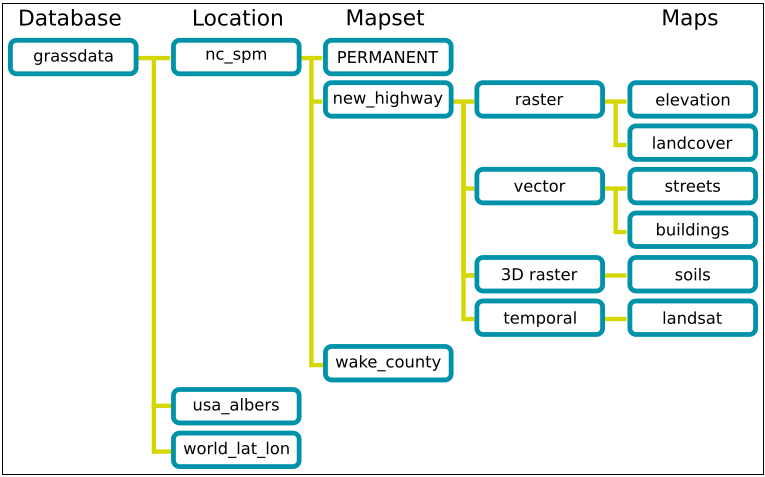
\includegraphics[width=14cm]{../pictures/grass_data_hiearchy.png} 
\caption[GRASS GIS 7 location structure]{GRASS GIS 7 location structure}
\label{fig:grass_data_hierarchy}
\end{center}
\end{figure}

\subsubsection{Startup screen versus splash screen}
\label{subsection:mechanism}
\noindent
\large
First, it is important to distinguish between the terms startup screen and splash screen. As Ed Foster stated in 1996: ``Splash screens, as they are commonly called, are the graphic logos that display while the program is loading and identify the program while reminding you about the software publisher's copyright restrictions." So, it appears before the main software window starts and remains visible for a few seconds. If we try to find articles on the startup screen, we will not be very successful. Nowadays, this topic lives mainly on programming websites such as Stack Overflow. In some software startup screen can mean at the same time a splash screen. However, generally speaking, a startup screen usually requires some initial action from the user to set up the software. 

The startup screen is the first component of the GRASS GIS version 7.8 that the user meets. It allows us to set all the above-mentioned components except \textit{Maps} and, in the case of \textit{Locations} and \textit{Mapsets}, also manage them in terms of renaming and deleting. The various historical versions of the startup screen can be seen in Figure \ref{fig:verze_startup}. The one on the right corresponds to the version 7.5 (as well as 7.8).

\vspace{0.3cm}
\begin{figure}[hbt!]
\begin{center}
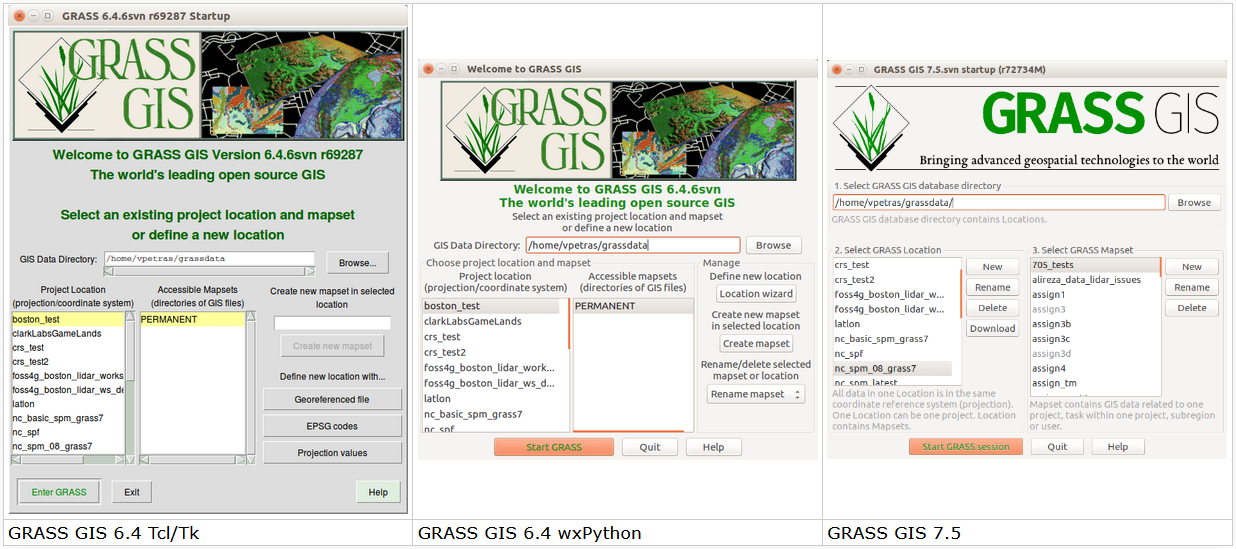
\includegraphics[width=17cm]{../pictures/verze_startup.png} 
\caption[Historical versions of the GRASS startup screen]{Historical versions of the GRASS startup screen}
\label{fig:verze_startup}
\end{center}
\end{figure}

\subsubsection{Location Wizard}
\label{subsection:wizard}
\noindent
\large
Location Wizard is a software component, which has the character of a guide which appears when creating a new \textit{Location} - collection of data with common CRS/SRS. Therefore, the main task of the wizard is to define this system. It consists of four consecutive dialog boxes, the one for selecting the coordinate system can be seen in Figure \ref{fig:loc_wizard_sour_pred}.

\vspace{0.3cm}
\begin{figure}[hbt!]
\begin{center}
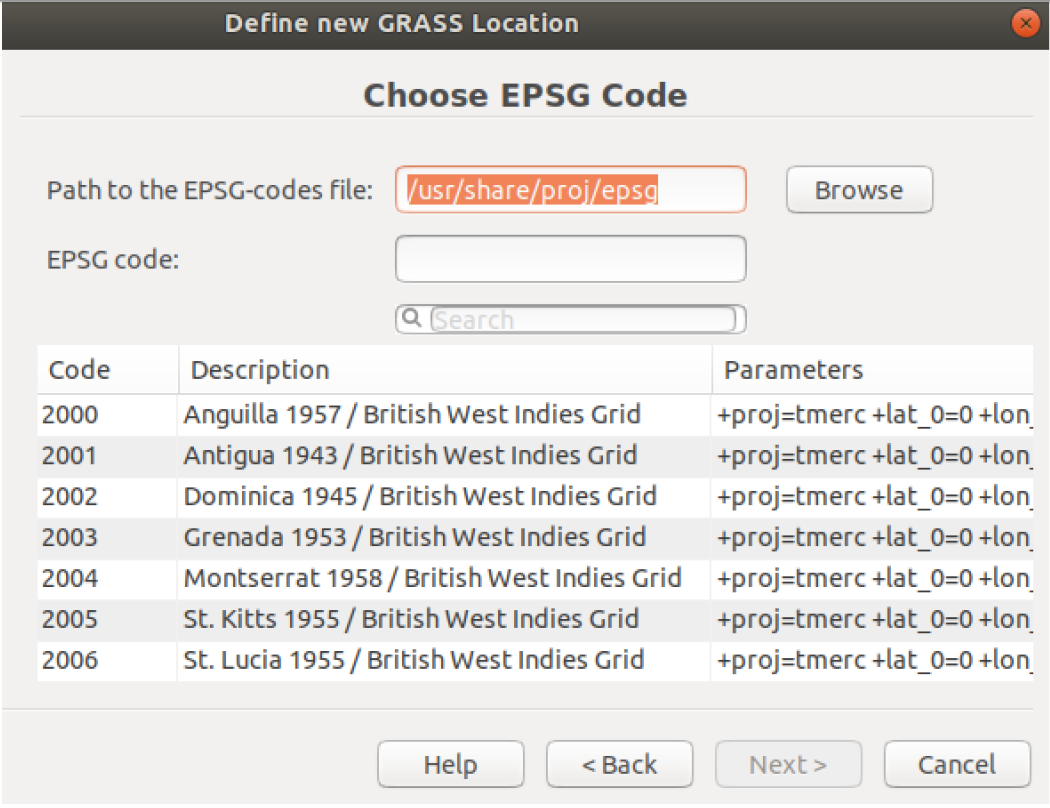
\includegraphics[width=10cm]{../pictures/loc_wizard_sour_pred.png} 
\caption[Choosing EPSG code in Location Wizard in version 7.8]{Choosing EPSG code in Location Wizard in version 7.8 (Source: Personal collection)}
\label{fig:loc_wizard_sour_pred}
\end{center}
\end{figure}

\newpage
\vspace*{-1cm}
\subsubsection{Layer Manager and Map Window}

\noindent The peculiarity of GRASS GIS is that it does not consist of one software window, as is usually the custom, but directly of two. The topic of connecting Layer Manager with Map Window is, by the way, another of the things that are likely to come. It is one of the proposed topics on GSoC \footnote{\url{https://trac.osgeo.org/grass/wiki/GSoC/2020\#GRASSGUI:Singlewindowlayout}}.

As explained in more detail in the documentation, Layer Manager provides a GUI for creating and managing \textit{Maps}. In Fig. \ref{fig:empty_layers1} we can notice five tabs - Layers, Console, Modules, Data and Python.

In the Layer Manager version 7.8, after running GRASS we first see the Layers tab, which allows layers in Map Display to be switched on and off. After starting the session this tab is empty. The path to the current \textit{mapset} and \textit{location} can be noticed in the top bar in the Map Display window. In this case, the current mapset is called \textit{demomapset} and is located in the location named \textit{fire\_grassdata}. GRASS GIS allows to add more Map Display windows. You can then manage layers in these windows via the Layers tab.
\vspace{0.3cm}
\begin{figure}[hbt!] 
\begin{center}
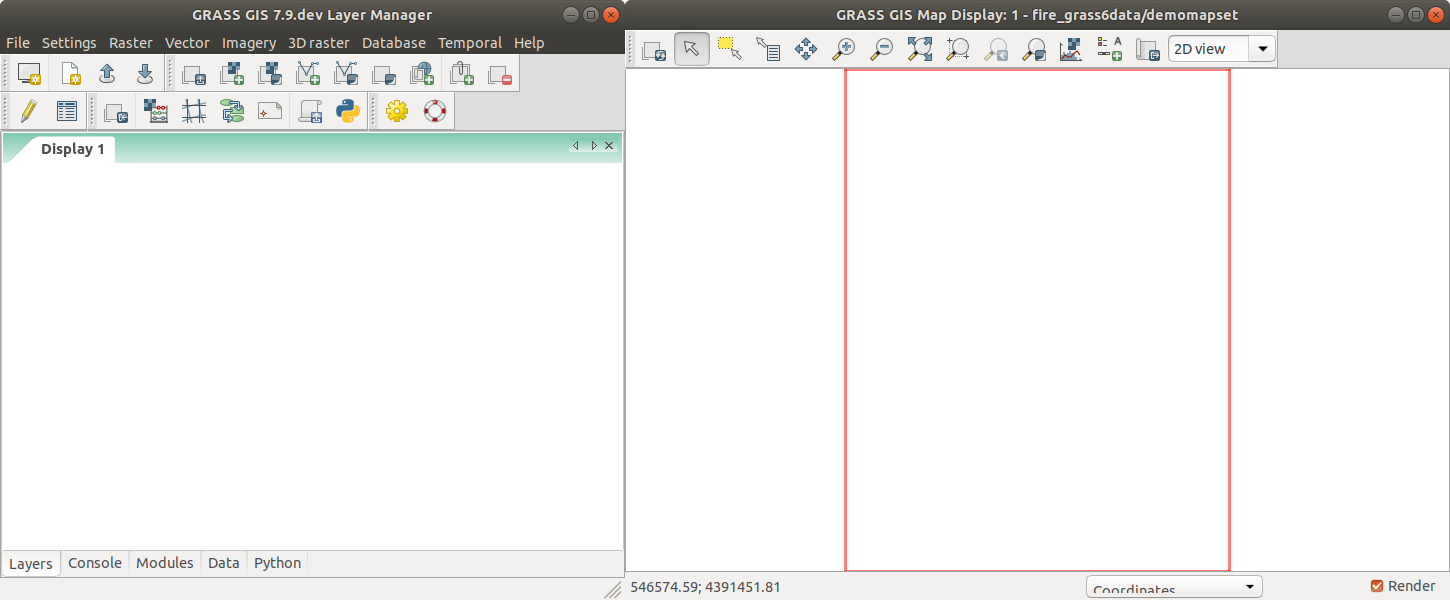
\includegraphics[width=17cm]{../pictures/empty_layers1.png} 
\caption[Layer Manager and Map Window (Version before GSoC)]{Layer Manager and Map Window  (Version before GSoC, Source: Personal collection)}
\label{fig:empty_layers1}
\end{center}
\end{figure}

\noindent In this work we will deal only with the Data tab, the explanation of other tabs can be found in the documentation \footnote{\url{https://grass.osgeo.org/grass79/manuals/wxGUI.html}}.
 
\newpage
\vspace*{-1cm}
\subsubsection{Data Catalog}

At the moment, when we want to display the data located in the current mapset, we need to go to the Data tab. In this tab provided in Figure \ref{fig:data_catalog_pred}, there is a Data Catalog (Data Tree) which very nicely captures the hierarchical structure of GRASS data. Within this tree we are allowed to work with \textit{maps} through context menu - to rename and delete them, display themselves or their metadata, or to copy them to another \textit{mapset}. This tab is therefore strongly associated with the organization of work in this software. However, in the version 7.8 Data Catalog does not provide management of mapsets, locations, or a database. Creating and changing a location and mapset is sort of hidden in the Settings/GRASS working environment tab.

The data in the so-called \textit{current mapset} (equal to active mapset) are firmly connected to the Map Display window. If we want to see maps from a different mapset we can find in mapset context menu the option for switching. We are able to switch between mapsets in the same location or between mapsets in different locations. If we move the data to the mapset in another location with a different coordinate system, the projection takes place. GRASS GIS does not use On the fly transformation.

\vspace{0.3cm}
\begin{figure}[hbt!] 
\begin{center}
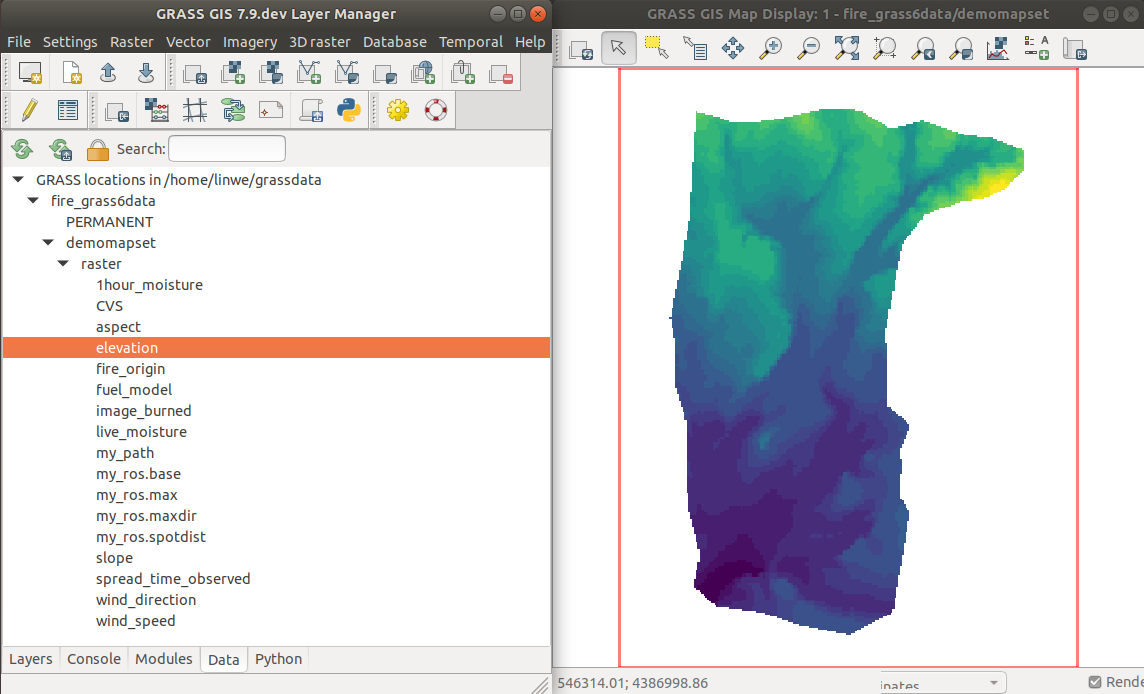
\includegraphics[width=17cm]{../pictures/data_catalog_pred.png} 
\caption[Data Catalog in Data tab (version before GSoC)]{Data Catalog in Data tab in the version before GSoC (Source: Personal collection)}
\label{fig:data_catalog_pred}
\end{center}
\end{figure}



\newpage
\vspace*{-1cm}
\subsubsection{Startup mechanism}
\label{section:mechanism}
\noindent
\large
This work talks about the startup mechanism, which is a concept that was introduced directly for the purposes of this work. No publications working with this term could be found. This is probably due to the facts that many software programs are developed commercially and most commonly used software or applications do not require any more complex initial setup. However, this is not the case here. It is therefore necessary to define what we consider by the term \textit{startup mechanism}.

\noindent The startup mechanism basically includes three things:

\begin {itemize}

\item the way the software can be started. In the case of GRASS GIS running under a Unix operating system, it is run from the command line.

\item components that the user encounters during startup. In the case of GRASS GIS version 7.8, these are the Startup screen, Location Wizard and Splash Screen. There may be situations where the requested mapset is locked (this happens if it is used by another process, or if the last session in this mapset ended in an error). If the running mapset is locked, we will be notified first after starting the Session that there is a lock file with a .gislock extension in the mapset, and then asked if we want to delete this file. In this special situation, when running GRASS, we even encounter five different components.
In the case of the version after GSoC, the mentioned components are bypassed in most situations and we can move straight to the third point.

\item state instantly after startup - here we can talk e.g. about the state of individual Layer Manager tabs,  about the state of Map Display, about new Info Bars for first-time user that will be implemented in this work, etc. 

\end{itemize}

\noindent From the point of view of the Layer Manager in the version 7.9, in fact, the Data tab (and subsequently the Data Catalog contained in it) is the most important os startup mechanism, as it is related to the organization of work in GRASS GIS. Correct and understandable setting of the data hierarchy is an important goal of the startup mechanism. Another no less important goal is to create a user-friendly environment in which the first-time user can quickly find his or her way around. This is, after all, the main topic of this master thesis.

\newpage
\vspace*{-1cm}
\fancyhead[RE, RO]{\fancyplain{}{\small \sl{State of Art}}}
\section{State of Art}
\label{State of Art}
\noindent
\large
The data hierarchy described in the previous section \ref{subsection:hierarchy} proves its worth especially when used by experienced users of GRASS, however, for complete beginners, it is rather confusing. Especially if the above-mentioned main components (database, location, and mapset) have to be defined right at the start of the software when launching the startup screen, which has been standard since version 6.4. 

Therefore, the general question was whether to keep data hierarchy at all or change the whole concept and use only \textit{project} and \textit{map} terms, which is the usual standard for other GIS software. The \texttt {database/location/mapset} mechanism may indeed seem complicated at first glance, but we must keep in mind that many later problems will be avoided by clearly defining the coordinate system at the beginning and allowing only one coordinate system within one location. From author’s point of view, the advantage (perhaps from the point of view of other users maybe the disadvantage) is that GRASS GIS does not support On the fly transformation. This may seem a bit rough at first, but it guarantees that we will not analyze data having a different coordinate system together, as could happen in ArcGIS or QGIS, for example. In these software, it can be confusing to see differently designed data in the right place on the map. In GRASS GIS, we also cannot get into a situation that the On the fly transformation does not occur at all, but even so it is allowed to display two layers of different coordinate systems on top of each other. This, of course, results in incorrect rendering of the layers in the map window (may happen e.g. in SAGA GIS).

Considering the disadvantages mentioned above, it seems very unfortunate to disrupt this system. Rather, it is important to clearly introduce it to newcomers. In the startup screen of version 7.8 (state before GSoC) there is a certain effort to provide the first-time user with the maximum possible help (short description of data hieararchy, Help button), but even so, the development community often encountered misunderstanding from the ranks of users \footnote{\url{https://trac.osgeo.org/grass/ticket/3474}}. 

Therefore, in 2017, the first suggestions on how to simplify this startup screen began to appear. In terms of implementation complexity, the simplest and most effective proposal seemed to be the A3 proposal. In Prague in 2019 an implementation proposal, also known as the Prague Roadmap\footnote{\url{https://trac.osgeo.org/grass/wiki/wxGUIDevelopment /New\ _Startup\#PragueRoadmap}}.  was created based on A3. A brief summary of the proposed implementation is contained in the next subchapter.

\newpage
\vspace*{-1cm}
\subsection{Prague Roadmap}
\label{section:Prague Roadmap}

The most serious changes concern the Data Catalog. They lie in supporting multiple databases, adding buttons to create existing or new databases, or adding new actions from the context menu to a database, location, and mapset node. The data hierarchy \texttt{database/location/mapset} is preserved and in addition, this proposal introduces a new concept called Workspaces which is not directly part of the Mapset, but is associated with it.

The same Data Catalog implemented in the Data tab is then planned to be used within startup screen inspired by A2 proposal designed by Garrett Millar. However, unlike the A2 design, the startup screen has no other tabs. It consists of only one startup page, which has a Data Datalog in the center, and a toolbar with big buttons for creating or defining new or existing hierarchy components, such as a location or mapset.

The proposed changes in the Location Wizard are mainly related to the clarification of the first page, better naming of the given attributes and speeding up the selection of the coordinate system in the dialog.

Furthermore, the proposal assumes the possibility of filtering in the Data Catalog based on the recently selected items. General startup GUI should be able to collect recent maps and workspaces as well as used databases and workspaces. The display of map layers in the Data Catalog is switched off by default, the display of workspaces under the relevant mapset is switched on. When GRASS GIS launches, a "grassdata" directory for storing locations, mapsets and maps should be automatically created in a reasonable place.


\subsection{Version 7.9 after Google Summer of Code}
\label{subsection:Version 7.9 after Google Summer of Code}
\noindent
The first part of this work focuses on a survey among intermediate users. One of the goals of this survey is to let users evaluate the changes in the version 7.9 after GSoC. Therefore, it is necessary to describe in detail what improvements Google Summer of Code has brought and in what is the appearance of the software at the time of the first survey.
Since the startup mechanism includes more or less interconnected software components that the first-time as well as experienced user will encounter almost one hundred percent at startup, the following subchapter is further divided into several smaller subsections. This time the software components are ranked according to their importance in version 7.9 after GSoC.


\newpage
\vspace*{-1cm}
\subsubsection{Data Catalog}

The main goal of GSoC was to improve the Data Catalog in such a way which enables a user-friendly organization of work. One may argue that these improvements are not related to the startup mechanism, but the truth is that the current version of the Data Catalog takes over the role of startup screen, and even offers more functionality. In the Figure \ref{fig:function} we can see the functions that have been newly implemented in the Data Catalog.

\vspace{0.3cm}
\begin{figure}[hbt!] 
\begin{center}
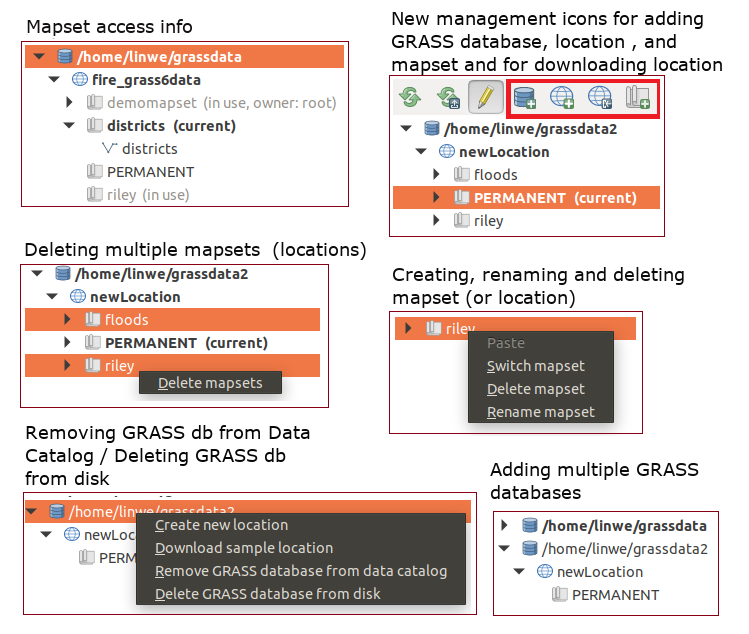
\includegraphics[width=15cm]{../pictures/funkce.png} 
\caption[New functionalities in Data Catalog ]{New functionalities in Data Catalog (Source: Personal collection)}
\label{fig:function}
\end{center}
\end{figure}

\noindent This is mainly about creating, renaming and deleting mapsets and locations, which was previously possible through the startup screen. However, completely new possibilities have been added. GRASS GIS allows a user to add multiple databases. New management icons offer intuitive creation of the mentioned data components. In the context menu there are also new options for deleting several mapsets or locations.

\newpage Though, probably the most visible changes are those related to the graphical representation of the Data Catalog. Next to the individual components, we can notice small icons distinguishing types of data hiearchy components. The Data Catalog also informs about access to individual mapsets (current, in use, and a different owner).

Another important thing is related to access to individual mapsets. In version 7.8, the startup screen informs about the lock and asks if the user wants to remove the lock.
In order to completely take over the startup screen functionality by the Data Catalog, it is also necessary to warn the user that the mapset to which they are going to switch is locked. How this case was solved is clear from the Figure \ref{fig:data_catalog_switch_new}. Because mapset locking was often confused with prohibiting editing outside the current mapset, the term was changed to \textit{mapset in use}. This term can also be seen in the Mapset Access Info in the Data Catalog.

\vspace{0.3cm}
\begin{figure}[hbt!] 
\begin{center}
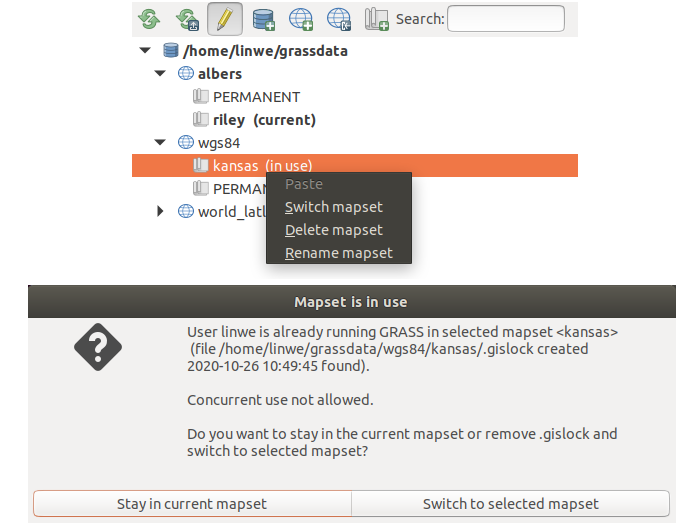
\includegraphics[width=13cm]{../pictures/data_catalog_switch.png} 
\caption[Switching to mapset in use in Data Catalog]{Switching to mapset in use in Data Catalog (Source: Personal collection)}
\label{fig:data_catalog_switch_new}
\end{center}
\end{figure}

\noindent Another important step forward was the graphic change of the icon enabling or disabling changes outside the current mapset. Now this icon has the character of a pencil (similar to QGIS) and protects a user from unwanted changes. If we do not have editing enabled, we cannot rename or delete any mapsets, locations and databases. We can only work with layers inside the current mapset. However, even if we enable editing, we can never delete a PERMANENT mapset. Similarly, we cannot delete boldly marked ``current” components in the Data Catalog.

\newpage
\vspace*{-1cm}
\subsubsection{Location Wizard}

This guide to creating new locations has been slightly modified and streamlined. In particular, we can see it on the first page ``Define a new GRASS location'' in Figure \ref{fig:loc_wiz_1}. Checkboxes and simplified names are removed here. The GRASS database can be newly modified.

\vspace{0.3cm}
\begin{figure}[hbt!] 
\begin{center}
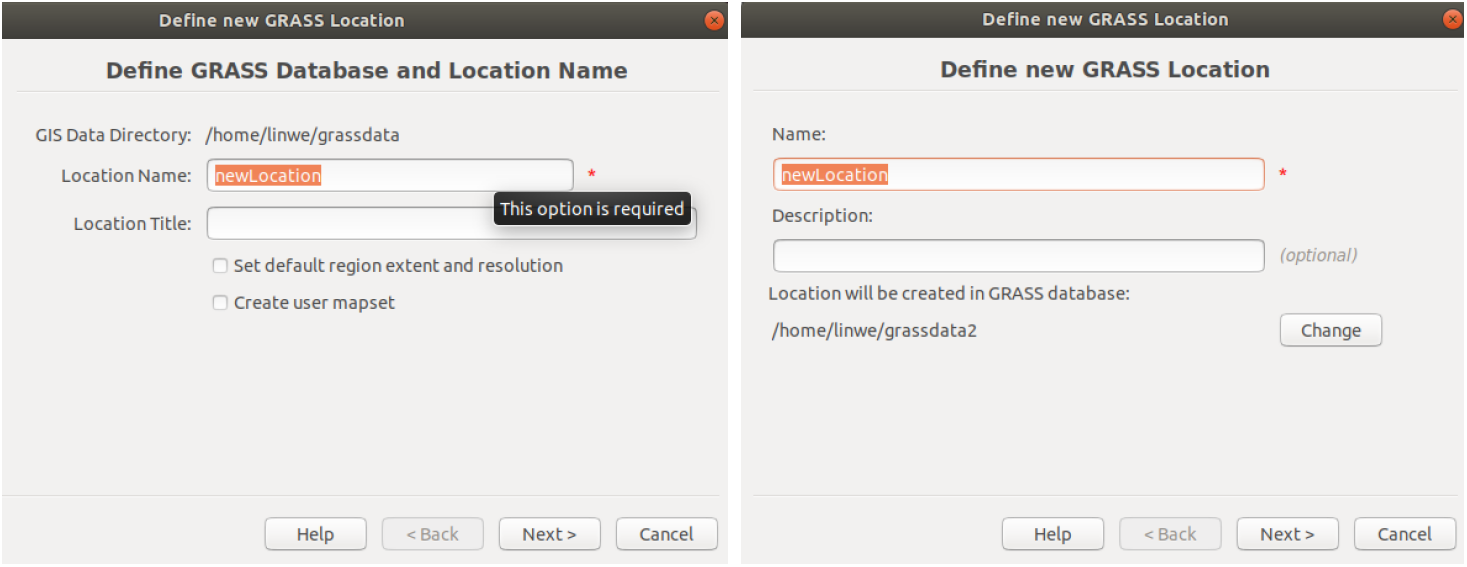
\includegraphics[width=17cm]{../pictures/loc_wiz_1.png} 
\caption[Location Wizard first page before and after GSoC]{Location Wizard first page before and after GSoC (Source: Personal collection)}
\label{fig:loc_wiz_1}
\end{center}
\end{figure}

\noindent The second page is renamed to ``Select Coordinate Reference System (CRS)''. As we can see in Figure \ref{fig:loc_wiz_2}, in the original version there is a division into simple and advanced methods, which is abolished in the new version. In addition, CRS can be newly specified using a WKT string.

\vspace{0.3cm}
\begin{figure}[hbt!] 
\begin{center}
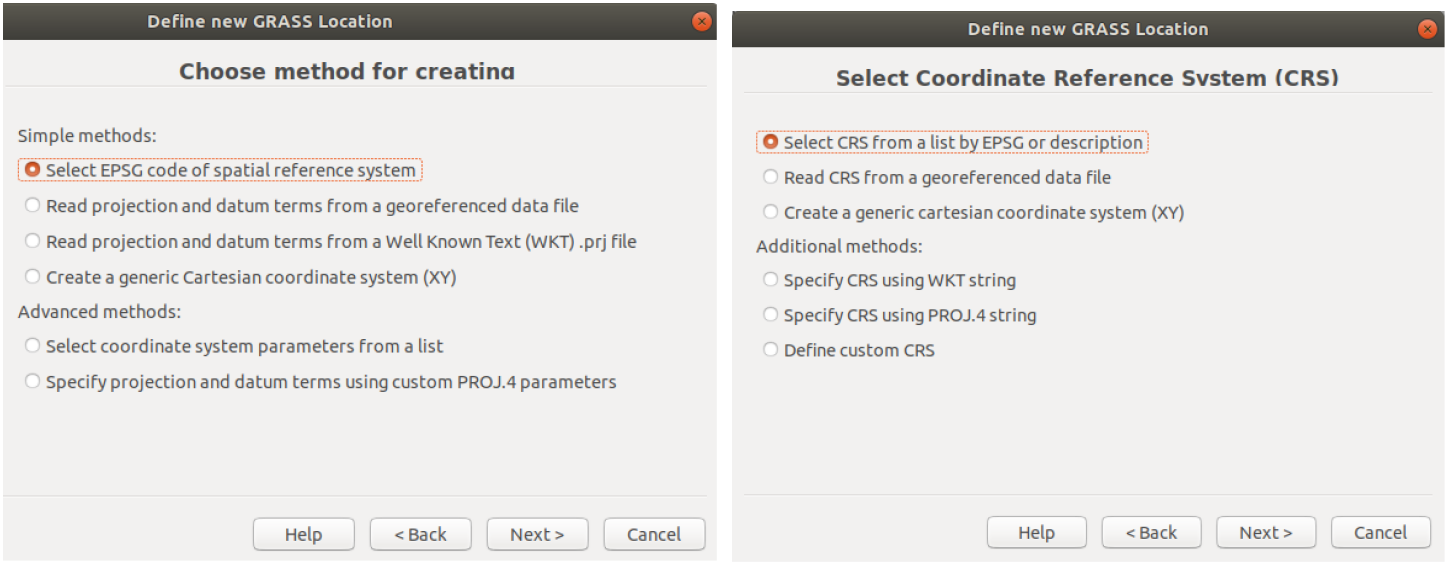
\includegraphics[width=17cm]{../pictures/loc_wiz_2.png} 
\caption[Location Wizard second page before and after GSoC]{Location Wizard second page before and after GSoC (Source: Personal collection)}
\label{fig:loc_wiz_2}
\end{center}
\end{figure}

\newpage
However, the essential change is related to ``Choose EPSG code'' page. Now it supports dynamic EPSG search. Furthermore, it provides the hyperlink to EPSG pages which is being changed dynamically according to a filter set by a user (see Fig. \ref{fig:loc_wiz_3}). The last page of the Location Wizard called ``Summary'' remains unchanged.


\vspace{0.3cm}
\begin{figure}[hbt!] 
\begin{center}
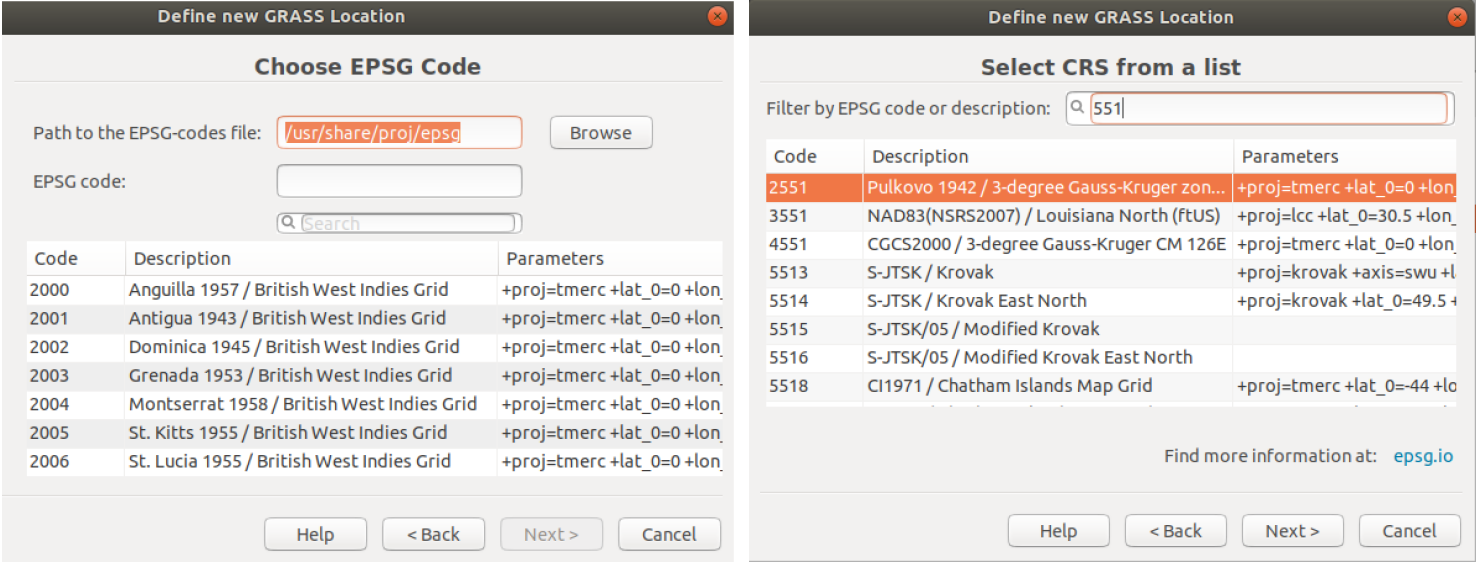
\includegraphics[width=17cm]{../pictures/loc_wiz_3.png} 
\caption[Location Wizard third page before and after GSoC)]{Location Wizard third page before and after GSoC (Source: Personal collection)}
\label{fig:loc_wiz_3}
\end{center}
\end{figure}

\vspace*{-1cm}
\subsubsection{Startup screen}

The changes that occurred during the Google Summer of Code were fundamental. At first, it was definitely not planned to remove the startup screen. The changes were to be based on Proposal A3, which planned to improve the Data Catalog, but also suggested that the same Data Catalog, which is available in the Data tab after starting the session, will be part of the startup screen.
During the implementation, however, all the functionality of the startup screen, including switching mapsets as well as locations and databases, was moved to the Data Catalog, so it no longer made sense to keep this notion. At least definitely not the form in which it is in the version 7.8.

\noindent We can encounter three different situations when starting the GRASS GIS ``after GSoC'' development version:

\begin{enumerate}

\item GRASS is launched directly with the Data Catalog visible in the prepared Demolocation (see Figure \ref{fig:demolocation_startup}). This situation occurs after the software is installed, that is, when no used databases are stored in the settings. Demolocation called \textit{world\_latlong\_wgs84} shows the correct organization of the data. Original data are stored in a permanent mapset whereas already analyzed data belongs to another mapset, for example to the one named after a user. The current implementation does not show a world map immediately at startup, it is necessary to display the map using Data Catalog (see Fig. \ref{fig:demolocation}).

\begin{figure}[hbt!] 
\begin{center}
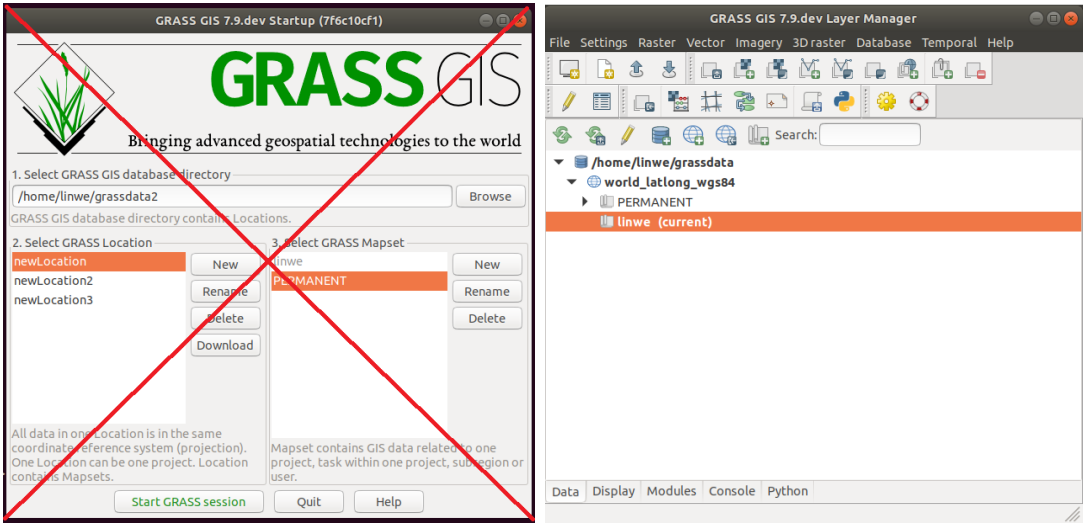
\includegraphics[width=17cm]{../pictures/demolocation_startup.png} 
\caption[GRASS launched with the Data Catalog in the prepared Demolocation]{GRASS launched with the Data Catalog in the prepared Demolocation (Source: Personal collection)}
\label{fig:demolocation_startup}
\end{center}
\end{figure}

\begin{figure}[hbt!] 
\begin{center}
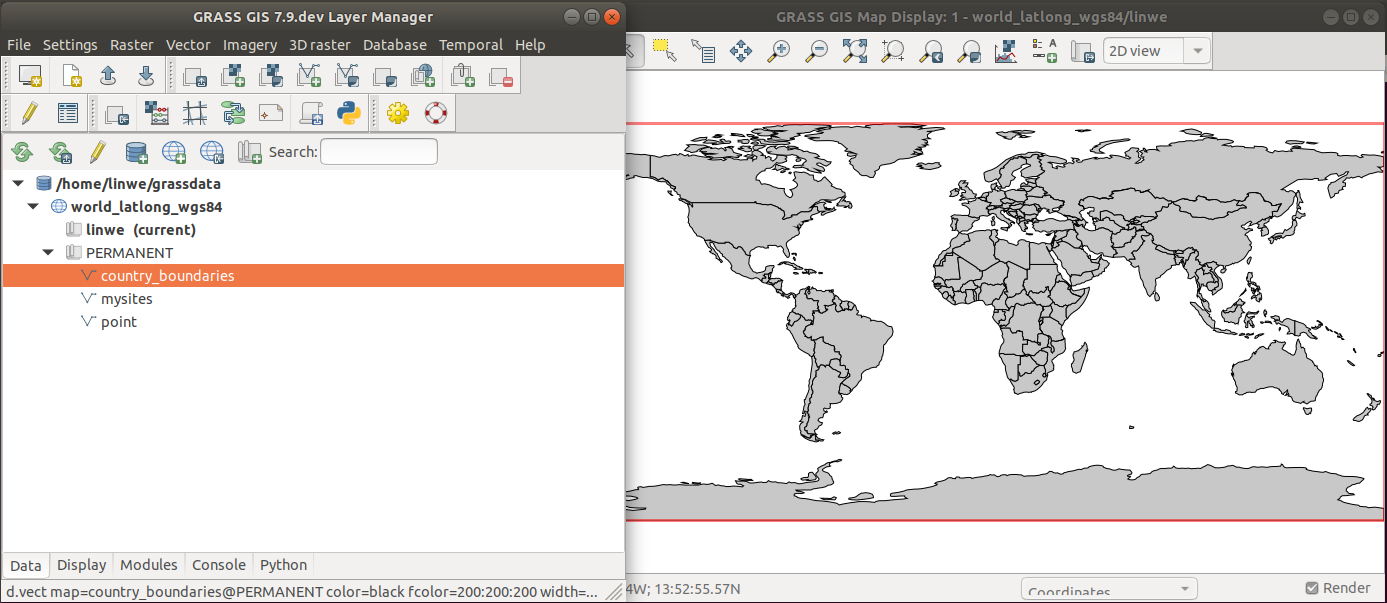
\includegraphics[width=16.5cm]{../pictures/demolocation.png} 
\caption[World map as a part of Demolocation]{World map as a part of Demolocation (Source: Personal collection)}
\label{fig:demolocation}
\end{center}
\end{figure}

\begin{figure}[hbt!] 
\begin{center}
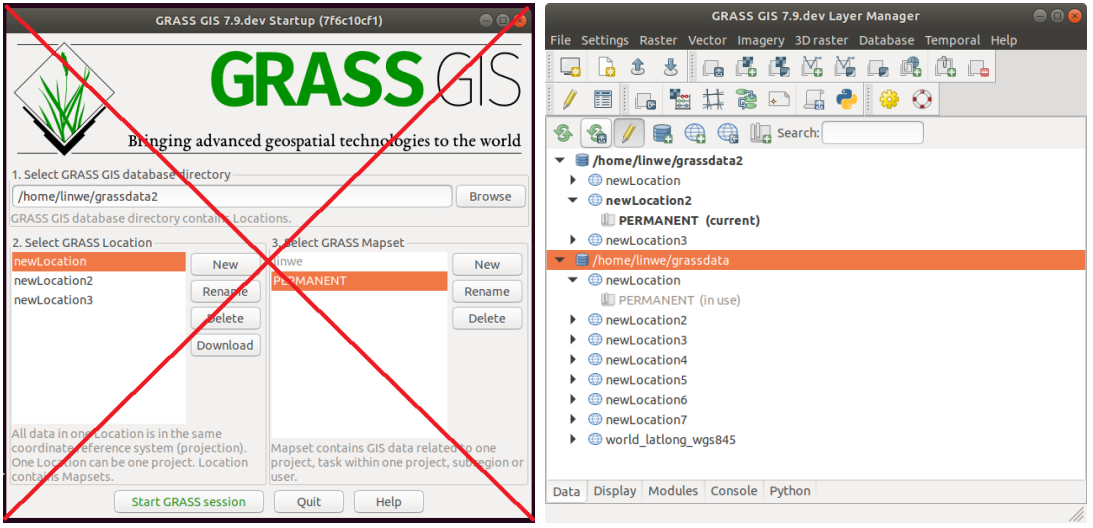
\includegraphics[width=16.5cm]{../pictures/last_mapset_startup.png} 
\caption[Data Catalog in Data tab (version before GSoC)]{Data Catalog in Data tab in the version before GSoC (Source: Personal collection)}
\label{fig:last_mapset_startup}
\end{center}
\end{figure}

\newpage
\item GRASS bypasses the Startup screen if possible to start in the last used mapset (see Figure \ref{fig:last_mapset_startup}). This situation is probably the most common. The software remembers the databases that were open when the last session was closed and opens them.
\item GRASS GIS launches in Startup screen if a mapset is not in a usable state (was deleted or is used by another process). In this special situation, GRASS starts in the same way as in the version 7.8.

\end{enumerate}

\subsubsection{Various options for starting GRASS}

\large \noindent In addition to the software components that the user encounters during startup and to the state that the software finds itself immediately after startup, the startup mechanism also includes the way we run the software. Because users of this software usually work under a Unix operating system, GRASS GIS is usually run from the command line. Advanced users often do not even run the graphical environment and perform all geographic analyzes using the command line. This is also why the command line window runs in the background throughout the work with this software. In our work, however, we mainly focus on first-time users who do not have to be experienced. This is also basically the main reason why we try to improve GRASS GUI.

 \noindent To summarize, the software could be run from the command line in four ways:

\noindent \texttt{:$\sim$\$ grass79} \\
\noindent Start GRASS using the default user interface. In the version 7.8, the user is prompted by the startup screen. After GSoC startup screen appears only when the mapset is not in the usable state.

\noindent \texttt{:$\sim$\$ grass79 --gui}\\
\noindent Start GRASS using the graphical user interface.  In the version 7.8, the user is prompted by the startup screen. After GSoC startup screen appears only when the mapset is not in the usable state.

\noindent \texttt{:$\sim$\$ grass79 --text} \\
\noindent Start GRASS using the text-based user interface. Appropriate location and mapset must be either set by environmental variables or taken from the last GRASS session.

\noindent \texttt{:$\sim$\$ grass79 --gtext} \\
\noindent Start GRASS using the text-based user interface.  In the version 7.8, this option as the only one does not display the Startup screen. However, it means that desired location and mapset must already be set as environmental variables, for example by running a specific mapset using the \texttt{:$\sim$\$ grass78 \$HOME/grassdata/location/mapset} command, or taken from the last GRASS session, specifically from a file in the path \textit{\$HOME/.grass7/rc}, which stores the current mapset and current location when the software is closed.
In the version 7.9, --gtext uses startup screen but then does not run the GUI.

There are two other topics related in part to starting the software. The first is the splash screen. In the new implementation, the splash screen does not appear during normal startup. The second thing that could further expand the possibilities of starting GRASS is the new concept of Workspaces. In the development version of the software version, it is possible to save the current software settings and then open it, as we can see in Fig. \ref {fig:workspace_grass}. However, there is no option to start a specific workspace from the command line or to start GRASS GIS from File Manager using the file association of the workspace file (.gxw).

\vspace{0.3cm}
\begin{figure}[hbt!] 
\begin{center}
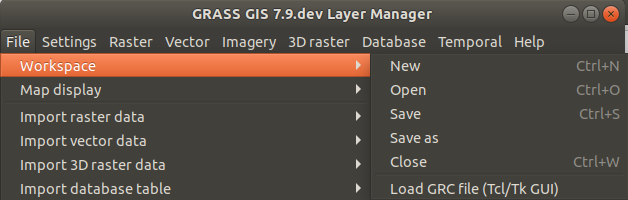
\includegraphics[width=14cm]{../pictures/workspace_grass.png} 
\caption[Management of Workspaces in the Layer Manager]{Management of Workspaces in the Layer Manager (Source: Personal collection)}
\label{fig:workspace_grass}
\end{center}
\end{figure}


\newpage
\vspace*{-1cm}
\subsection{Suggestions for improvement}

After GSoC, two fundamental questions arose, to which we will try to find answers in this work:

\begin{enumerate}

\item  \noindent \textbf{Would be implementing a special mode for first-time user helpful? What should this first-time mode look like?}

\noindent As mentioned at the beginning of this chapter, data hierarchy in GRASS GIS can cause significant problems for newcomers. Therefore, the core question of this work is how to enhance the first-time user experience.

\item \noindent \textbf{How to start GRASS in a special situation when the last opened mapset is not in the usable state?}

As mentioned in the previous chapter, in the special situation where the last opened mapset is not in the usable state (is in use or was deleted), the ``old'' startup screen still appears. This situation is rather a lack of a new solution and one of the goals of this work is to eliminate this shortcoming. 

\end{enumerate}

\noindent Other questions can be:

\begin{enumerate}
\setcounter{enumi}{2}

 \item \noindent Should the world map automatically appear in the Map Display when Demolocation starts?
 
 \item \noindent What other functions to add to the Data Catalog?
 
 \item \noindent Does it make sense to add a file association of the workspace file (.gxw) in order to be able to start GRASS GIS from File Manager?
  
\item \noindent How to solve starting with the command \texttt{:$\sim$\$ grass78 --gtext}? Cancel or keep and run g.gui.datacatalog instead of the old startup screen?
 
\end{enumerate}

\noindent The aim of this work is to find answers to the above questions, to propose a solution and in the case of first two questions also to implement it. The solution will be compiled on the basis of two different sources - according to trends in current GIS software and especially according to the results of the two surveys among differently experienced users. The first survey is focused on the improving of the startup mechanism and finding ways how to improve first-time user experience. As feedback from users is very valuable, the aim of the first survey in particular is to find out, among other things, how satisfied users are with the new state after GSoC. Similarly the second survey conducted one month later finds out whether users like the newly designed mockups of Info Bars for first-time users and gives them space to share their own ideas so that the implemented solution is the best possible from an objective point of view.

%% -------<<< Chapter 2: Concepts of startup mechanism >>>-------\\%%%%%%%%%%%%%%%%%%%%%%%%%%%%%%%%%%%%
\newpage
\vspace*{-1cm}
\fancyhead[RE, RO]{\fancyplain{}{\small \sl{General startup concepts}}}
\section{General startup concepts}
\label{sec:startup_concepts}
\noindent
\large
As the author already mentioned, the most commonly used software or applications usually do not require any more complex initial setup. However, this may not be the case for GIS software. Therefore, the following subsection introduces and compares several GIS approaches in terms of startup mechanisms. Then we move even beyond GIS and look especially on the way, how software programs chosen according to the first survey enhance the first-time user experience.

\subsection{GIS software}
\label{subsection:GIS software}

The startup mechanisms are analyzed from various perspectives, which are summarized in the final table identifying several questions:
\begin{itemize}
\item Does the GIS software have its own startup screen, and if so, how does it look like? 
\item Does the software have file association of project file?
\item Does the software offer first-time mode to help complete beginners, and if so, in what form?
\item How the software works with data of different coordinate systems? Does it support On the fly transformation? Does it allow the incorrect display of two layers of different coordinate systems on top of each other?
\end{itemize}

\noindent On Figures \ref{fig:hodnoceni_all} and  \ref{fig:hodnoceni_free} we can see graphs of the 10 highest rated GIS software and the 10 highest rated Free GIS software in the world in 2020, as stated in the evaluation taken by online magazine GISGeography. The evaluation of selected software is performed on a point scale from 0 to 10 in four categories - \textit{cartography, analysis, editing and data management} which are subsequently averaged. 

In the first place we can notice two representatives of ESRI - ArcGIS Pro, ArcGIS Desktop. I would also mention the other two interesting commercial software GeoMedia (Hexagon) and MapInfo Professional. If we focus only on Free GIS Software, in the first places in descending order we can find QGIS 3, QGIS 2, gVSIG, GRASS GIS, ILWIS and SAGA GIS. 

\vspace{0.3cm}
\begin{figure}[hbt!] 
\begin{center}
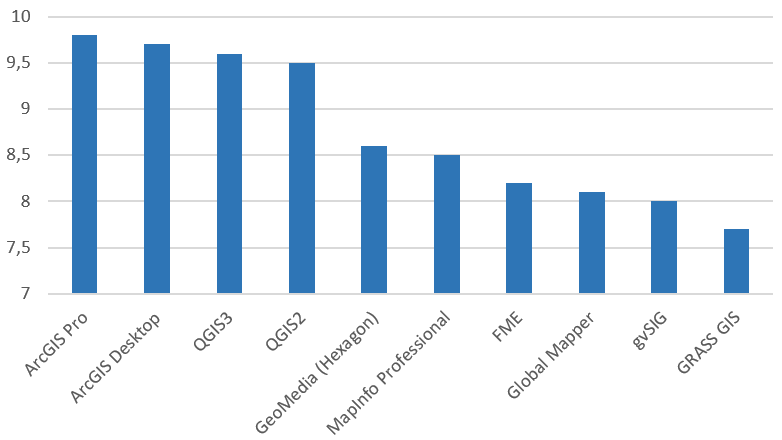
\includegraphics[width=13cm]{../pictures/hodnoceni_all.png} 
\caption[Top 10 GIS Software in 2020 according to GISGeography journal]{Top 10 GIS Software in 2020 according to GISGeography journal}
\label{fig:hodnoceni_all}
\end{center}
\end{figure}

\begin{figure}[hbt!] 
\begin{center}
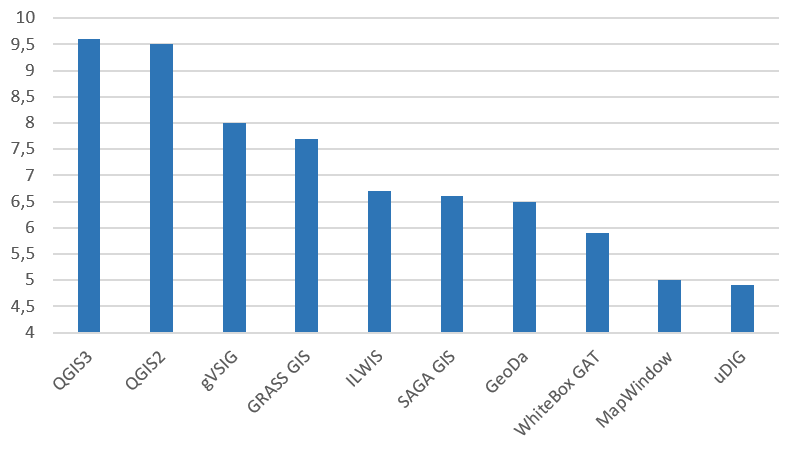
\includegraphics[width=13cm]{../pictures/hodnoceni_free.png} 
\caption[Top 10 Free GIS Software in 2020 according to GISGeography journal]{Top 10 Free GIS Software in 2020 according to GISGeography journal}
\label{fig:hodnoceni_free}
\end{center}
\end{figure}

\newpage
\noindent We must keep in mind that this evaluation is very indicative, as each software has different strengths. For example, on Figure \ref{fig:hodnoceni_analysis} GRASS GIS takes the leading position in then \textit{analysis} category, with a rating of 9.8 out of 10, which is comparable to FME and ArcGIS Pro. Among Free GIS Software GRASS has the highest rating in this aspect. This uniqueness is also mentioned in the pros of the software, which offers more than 350 geoprocessing modules, LiDAR and network analysis, sophisticated tools for satellite imagery, 3D raster rendering and customization and so forth.  The big advantage is that the GRASS GIS function can be leverage through QGIS or uDig. 

\newpage
In the disciplines of editing and data management, the balance is somewhat worse 7.4 and 7.5 out of 10 points. The biggest drop to 6.1 is in the \textit{cartography} category. At this point, however, it must be highlighted that the ambition of GRASS GIS is definitely not to create high-quality modern maps, but to offer the software for very numerically complex geographical analyzes. What is mentioned as other disadvantages is clunky and dated user interface, defining projects on start-up, steep learning curve to get started and command line window running in background. We can notice that these shortcomings are largely related to the current unfortunate startup mechanism.

\begin{figure}[hbt!] 
\begin{center}
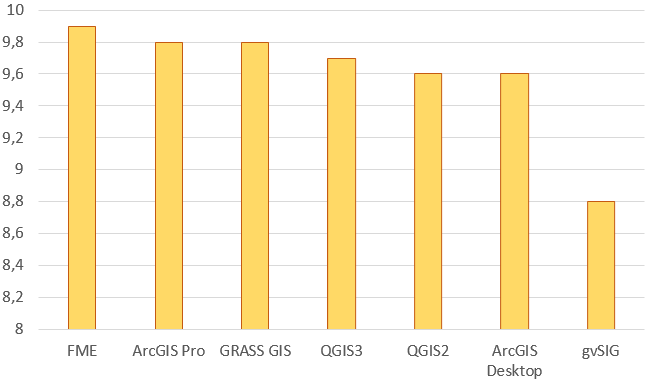
\includegraphics[width=11cm]{../pictures/hodnoceni_analysis.png} 
\caption[Top 7 GIS Software in 2020 in \textit{analysis} category according to GISGeography journal]{Top 7 GIS Software in 2020 in \textit{analysis} category according to GISGeography journal}
\label{fig:hodnoceni_analysis}
\end{center}
\end{figure}

\noindent At this point, it is important to emphasize that in this work we do not focus at all on the functionality of the software as such. As you could read in the previous lines, in this aspect the software is really very different. Therefore, even though the software may not be very user-friendly, a user will have no choice and reach for it. In this work, software is tested and analyzed in detail from the point of view of the startup mechanism and data organization with an emphasis on finding out what elements they use directly in the software to improve the first-time user experience.

The software is tested using two shapefiles of different coordinate system - districts in the Czech Republic in the S-JTSK Krovak East North system (EPSG: 5514) and US tracts in the USA Contiguous Albers Equal Area Conic system (ESRI: 102003). These systems are not selected by chance. They are defined entirely differently, however, in terms of coordinate digits they are very similar.

The author has extensive experience with ArcMap and QGIS, with other software she had the honor of working for the first time. However, for the purposes of this work, this fact is a plus, as the evaluation of software is not distorted by any previous experience.

\newpage
\vspace*{-1cm}
\subsubsection{Analysis of selected commercial software}

\noindent On further rows three commercial representatives (ArcGIS Pro, MapInfo Professional and GeoMedia Advantage) are described in terms of startup mechanisms, new user friendliness and data organization. Data import is also tested for each software. 

\bigskip

\noindent \textbf {ArcGIS Pro 2.4}

\noindent This software is currently the lead representative of ESRI's desktop GIS. It is an extension and connection of ArcMap, ArcScene and ArcGlobe applications. It is therefore possible to display and analyze 3D data in it. After logging in, the startup screen is displayed (see Figure \ref{fig:arcgis_startup_screen}). Here we can open recently saved projects or select from pre-prepared templates, of which we have several to choose from - Map (standard), Catalog, Global scene and Local scene. Another option is to select an empty sheet.

\vspace{0.3cm}
\begin{figure}[hbt!] 
\begin{center}
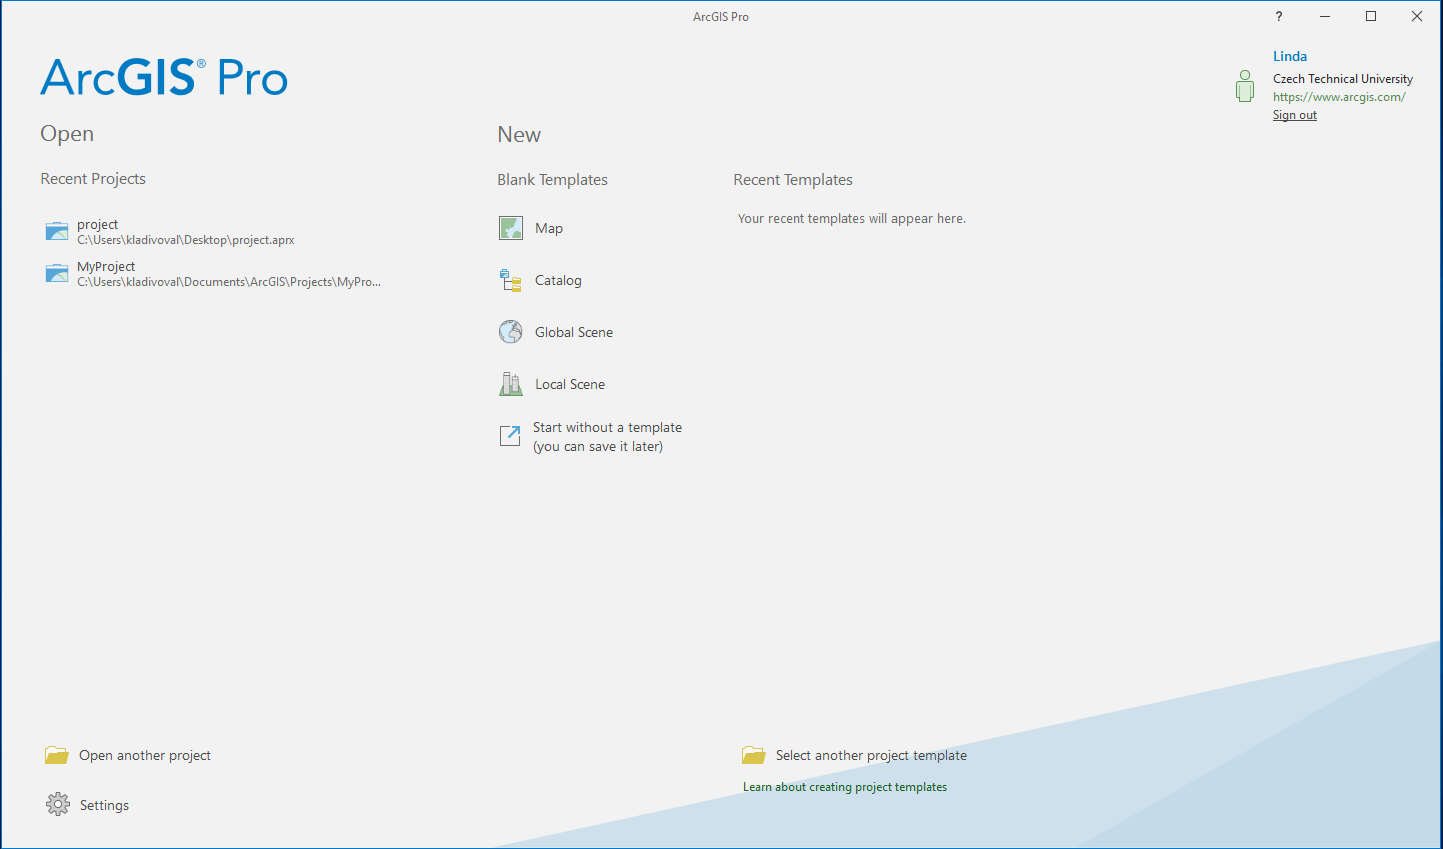
\includegraphics[width=16cm]{../pictures/arcgis_startup_screen.png} 
\caption[ArcGIS Pro 2.4 startup dialog]{ArcGIS Pro 2.4 startup dialog (Source: Personal collection)}
\label{fig:arcgis_startup_screen}
\end{center}
\end{figure}

\noindent The imported GIS layers are located in the Map component which is associated with Map window. In the following example on Figure \ref{fig:arcgis_pro_onthefly2}, the map window system is WGS 1984 Web Mercator Auxiliary Sphere (according to the first added layer), but the later layers added are in other coordinate systems. In spite of having different coordinate systems, the layers are displayed correctly in the map window due to On the fly transformation.

\newpage
\begin{figure}[hbt!] 
\begin{center}
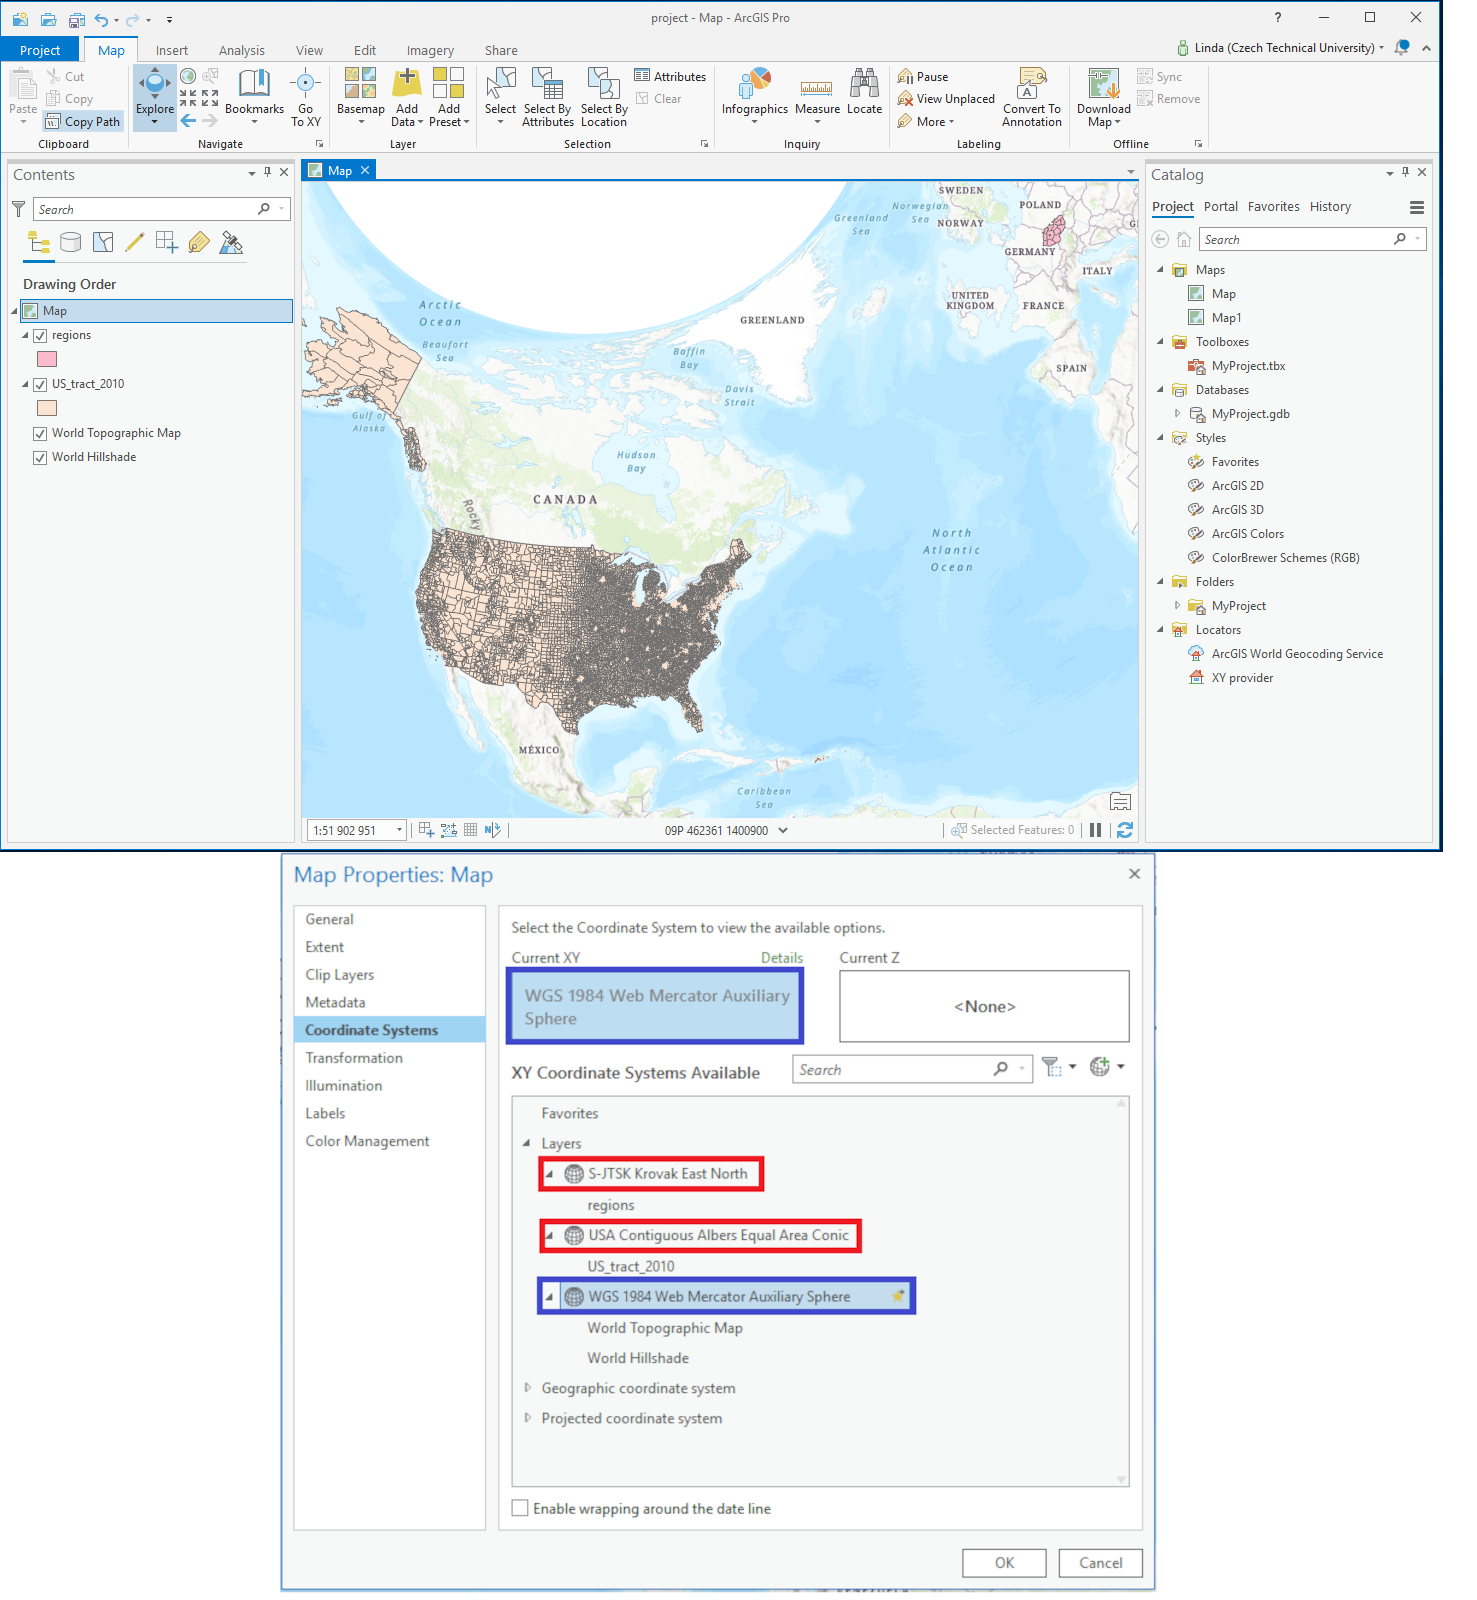
\includegraphics[width=16cm]{../pictures/arcgis_pro_onthefly2.png} 
\caption[Display of layers with different coordinate system in ArcGIS Pro 2.4]{Display of layers with different coordinate system in ArcGIS Pro 2.4 (Source: Personal collection)}
\label{fig:arcgis_pro_onthefly2}
\end{center}
\end{figure}

\noindent ArcGIS Pro works with projects as key elements of data organization. Each project contains a folder that contains the data we want to work with. So there is pressure to make data clear and not scattered all over the disk. We can say that ESRI is moving in a similar direction to GRASS GIS in this aspect. In the case of this software, it is not a disadvantage that it does not offer any special elements or explanations that could help newcomers. The startup screen and the software as such are at first glance clear and user friendly.

\newpage
\vspace*{-1cm}
\bigskip
\noindent \textbf {GeoMedia Advantage 2020}

\noindent This commercial GIS software developed by Intergraph (now Hexagon Geospatial) has a rich 40-year history. It is especially strong at cartography and raster analysis.  It also offers a unique 3D experience for viewing and analyzing data.

After complicated license setup (it is not possible to simply try the trial version, it is necessary to apply for a time-limited license key), we are greeted by a small start dialog captured in Figure \ref{fig:geomedia_startup}, where we can create our own GeoWorkspace file or open an existing one.

\vspace{0.3cm}
\begin{figure}[hbt!] 
\begin{center}
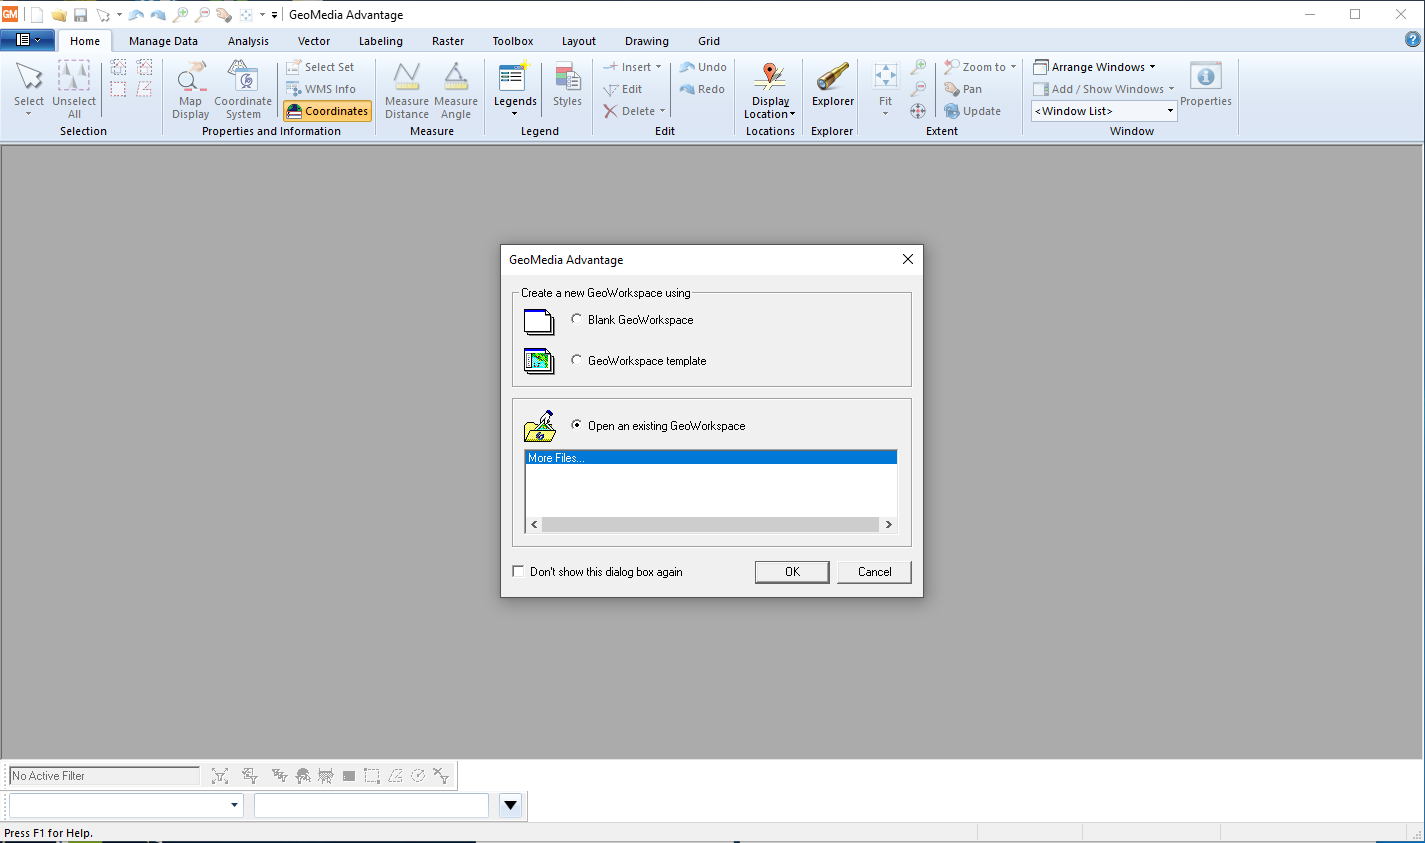
\includegraphics[width=17cm]{../pictures/geomedia_startup.png} 
\caption[GeoMedia Advantage 2020: startup dialog]{GeoMedia Advantage 2020: startup dialog (Source: Personal collection)}
\label{fig:geomedia_startup}
\end{center}
\end{figure}

\noindent Fortunately, the software provides two examples of GeoWorkspaces which give a user at least a little idea of how it all works. However, if we want to add our own data, it is very user-unfriendly and the author managed to do it after half an hour of intensive efforts.

Any external data we want to add to the software has a character of Warehouses. For example, to be able to display shapefiles (but also other formats), a user has to first define a Warehouse Configuration File. It consists of a data server definition (in the case of ArcView shapefile), a working folder with data and a coordinate system definition, see Figure \ref{fig:define_config_geomedia}. GeoMedia, like GRASS, also requires the definition of CRS right at the beginning and provides detailed settings for this purpose.

\vspace{0.3cm}
\begin{figure}[hbt!] 
\begin{center}
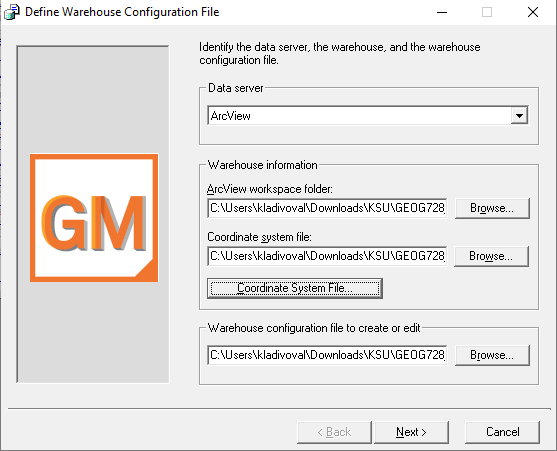
\includegraphics[width=13cm]{../pictures/define_config_geomedia.png} 
\caption[GeoMedia Advantage 2020: Define Warehouse Configuration File dialog]{GeoMedia Advantage 2020: Define Warehouse Configuration File dialog (Source: Personal collection)}
\label{fig:define_config_geomedia}
\end{center}
\end{figure}

\noindent In the next step it is needful to connect this configuration file. Once it is connected we can manipulate with data in a map window as with legend entries. Each GeoWorkspace file can have multiple Warehouses with different coordinate systems attached. In the map window, an On the fly transformation takes place according to the coordinate system of the map window, which is set under the term Location.

The software does not provide any help, so the user is completely clueless and forced to search the Internet. From a learning point of view, this software is definitely the most difficult to understand from the three selected commercial software. However, we can perceive a certain similarity with GRASS, especially in the setting of the coordinate system, which is also very important from the point of view of GeoMedia software. However, the map window supports the On the fly transformation, which is a significant difference from GRASS GIS.

\newpage
\vspace*{-1cm}
\bigskip

\noindent \textbf {MapInfo Professional 2019}

\noindent This commercial GIS software is developed by the American company Pitney Bowes, in the Czech Republic the exclusive provider is CS Map. As the name suggests, MapInfo is very strong in geodata visualization. it offers functionalities for doing modern cartography - several prepared map layouts, advanced labelling, accessing symbology etc. However, some analytical functions e. g. focused on LiDAR and remote sensing are missing.

When we run the software, we are redirected to the startup screen, which atypically occupies the size of the entire computer screen. The startup provides links to new version news or links to videos on YouTube that can help first-time users. In the upper right part of the startup screen it is possible to run help, which has the character of a separate desktop application. In the left part there is a simple bar allowing to choose a workspace we want to work in. We can open an empty workspace, sample workspace with a map of Washington DC or choose another previously saved workspace in the directory path. If we run the software again, the Open Last Saved Session option will be added to the startup screen.

\vspace{0.3cm}
\begin{figure}[hbt!] 
\begin{center}

\includegraphics[width=16cm]{../pictures/map_info_startup_screen.PNG} 
\caption[MapInfo Professional 2019 startup dialog]{MapInfo Professional 2019 startup dialog (Source: Personal collection)}
\label{fig:map_info_startup_screen}
\end{center}
\end{figure}

\noindent As in ArcGIS Pro, the main component is the Map, which has one coordinate system defined. Data import is somewhat non-intuitive and must be demonstrated through the Open Table icon. When importing, a new file of company's own geodata format * .tab is created. We can define new projection or keep the original one. Coordinate system of the Map can be changed through Map Options as shown on Figure \ref{fig:map_info_startup_projection}. 

\vspace{0.3cm}
\begin{figure}[hbt!] 
\begin{center}
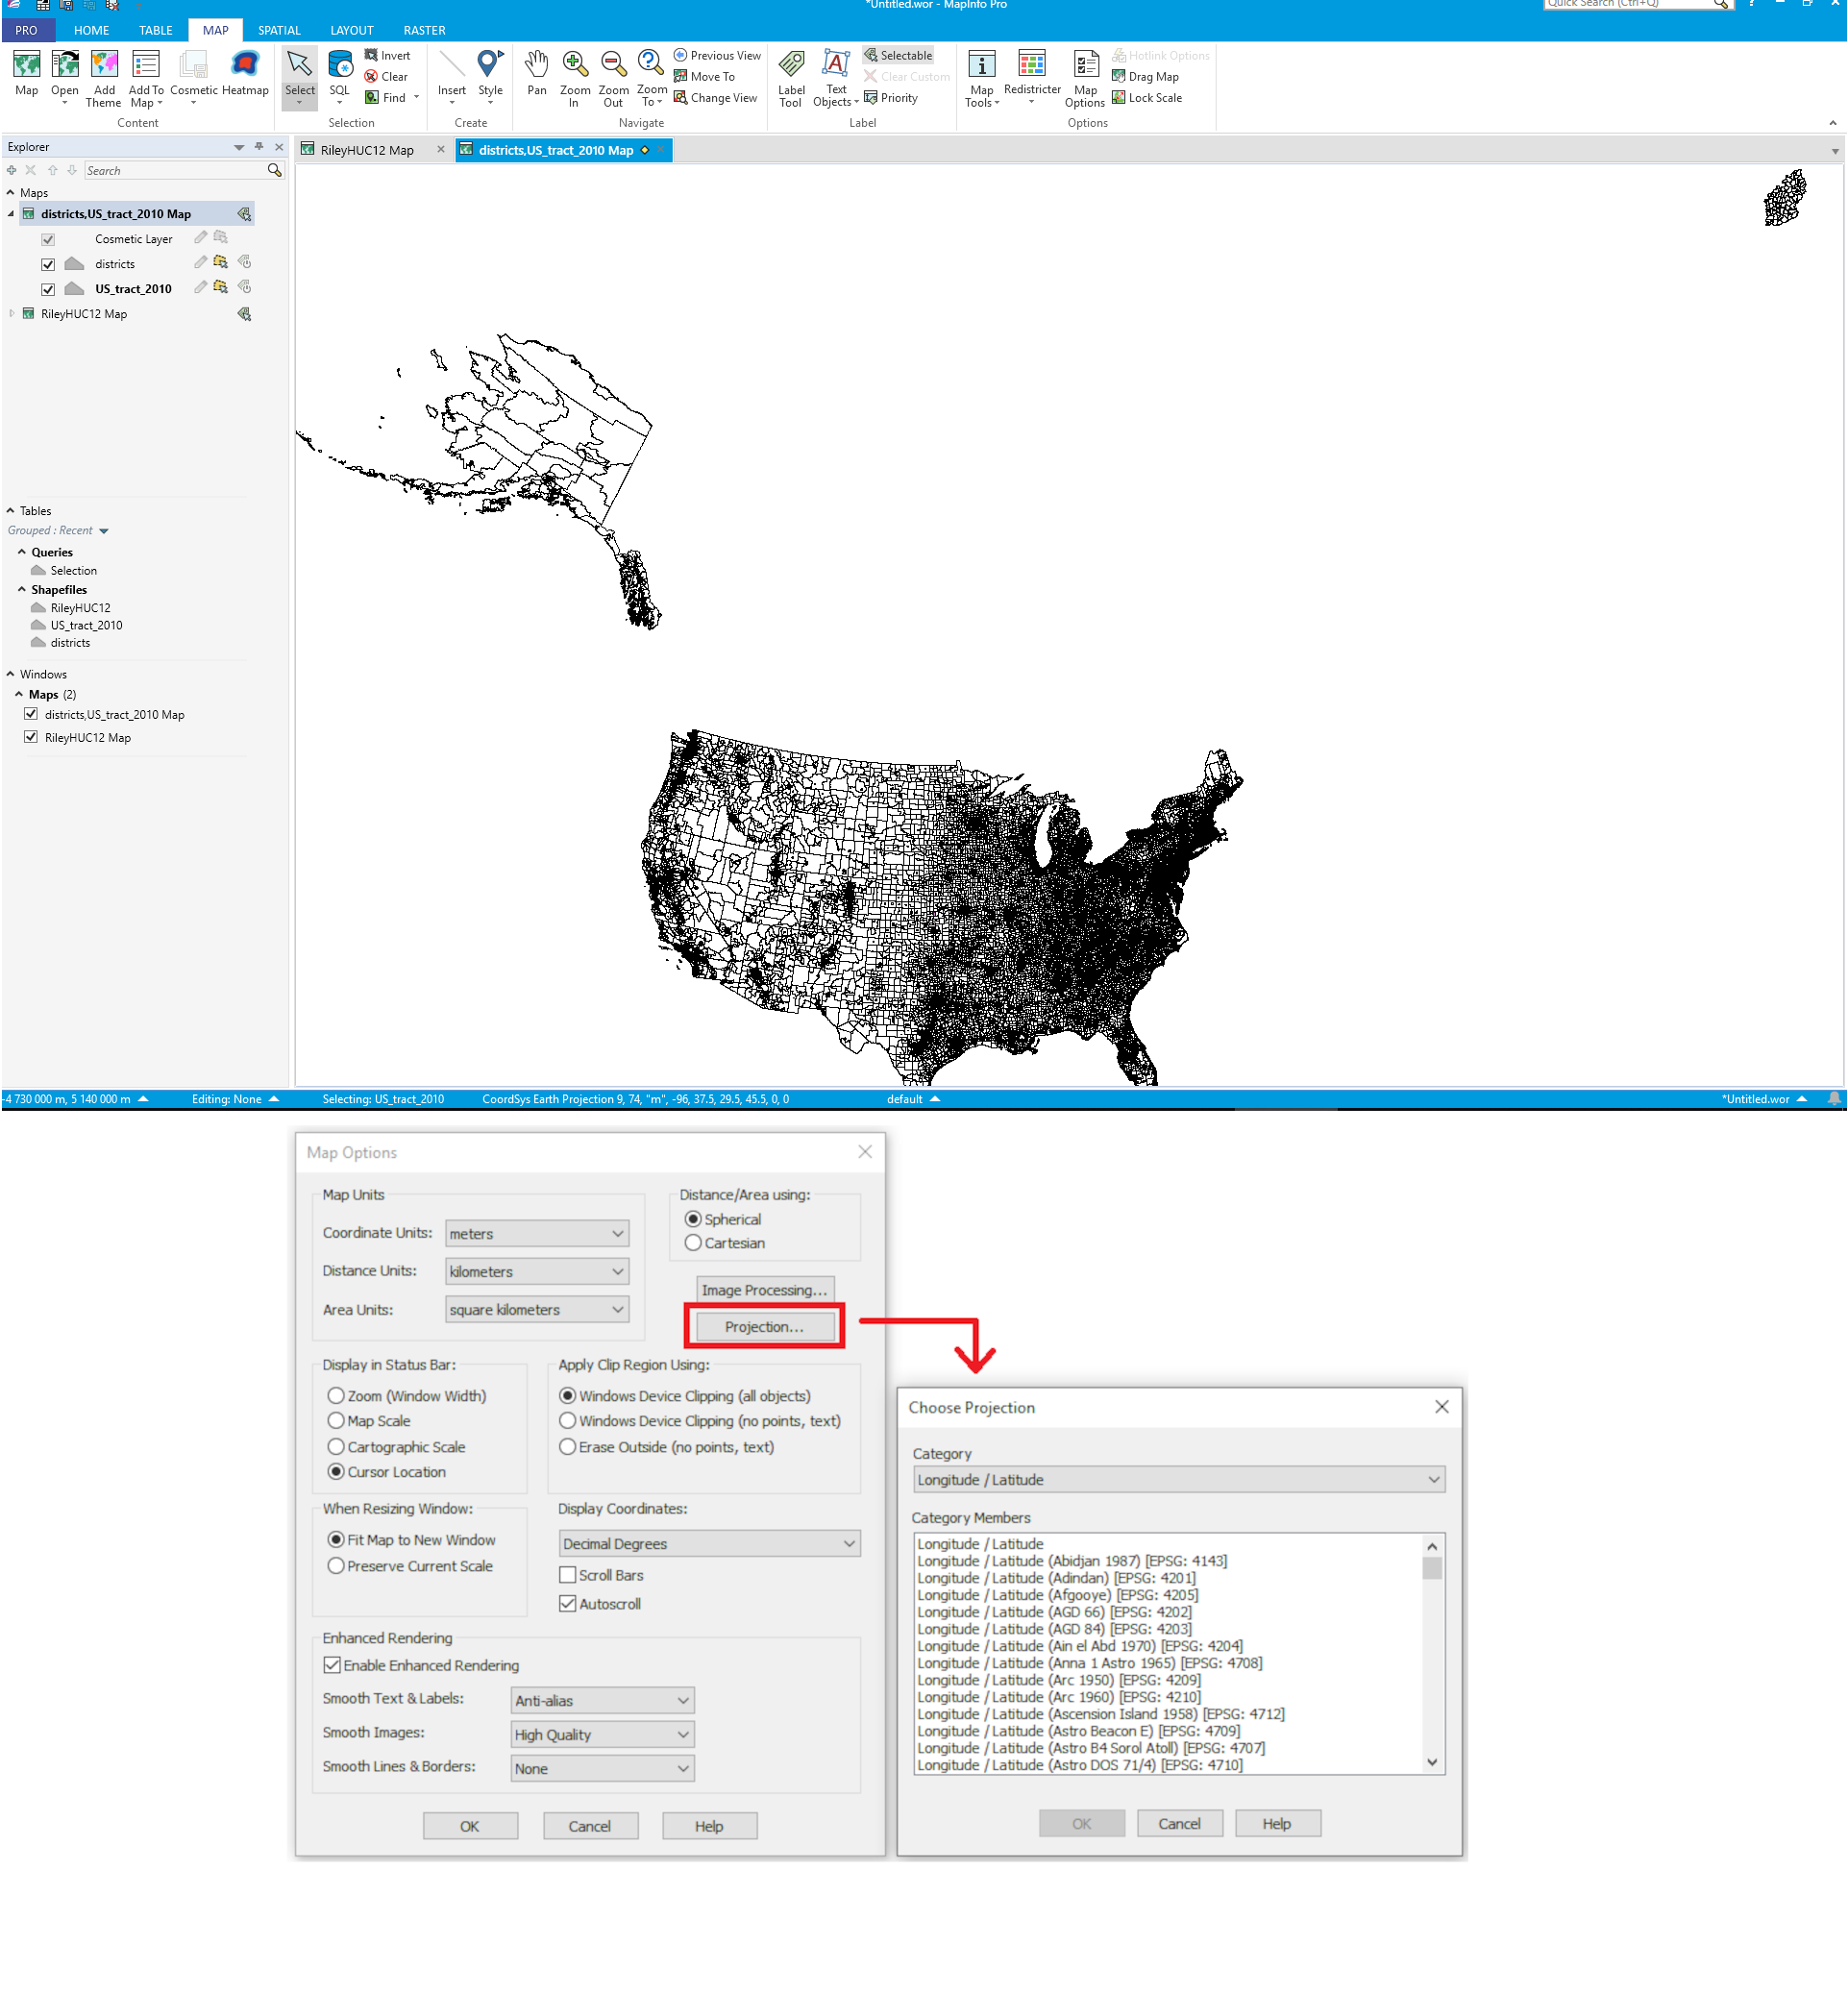
\includegraphics[width=16cm]{../pictures/map_info.PNG} 
\caption[Map-level coordinate system settings in MapInfo Professional 2019]{Map-level coordinate system settings in MapInfo Professional 2019 (Source: Personal collection)}
\label{fig:map_info_startup_projection}
\end{center}
\end{figure}

\noindent However, at first glance it is not clear in which coordinate system the layers are, more precisely whether we made On the fly transformation or data transformation. After a longer examination, it is clear that we transformed MapInfo *.tab file. The coordinate system is set to the map level (not layer level) and takes over the system of the first map layer added. 

\newpage
\vspace*{-1cm}
\subsubsection{Analysis of selected open-source software}

\noindent On further rows four open-source software (QGIS 3, gvSIG, ILWIS, SAGA GIS) are tested and analyzed in detail from the point of view of the startup mechanism with an emphasis on finding out what elements they use directly in the software to improve the first-time user experience. In the next chapter, the results of these analyzes are summarized in tables.

\bigskip

\noindent \textbf {QGIS 3.14}

\noindent This software is created similarly to GRASS GIS under the auspices of OSGeo. The big change from QGIS 2 is that it includes native support for 3D visualizations. The advantage is also the possibility of using and creating tailor-made plugins. QGIS also allows the use of analytical functions from GRASS, SAGA GIS software and the GDAL library. 

At the first start, Welcome to QGIS window appears, in which we can link to the QGIS website and check the news in the given version. The window runs in the default language of the operating system.

\vspace{0.3cm}
\begin{figure}[hbt!] 
\begin{center}
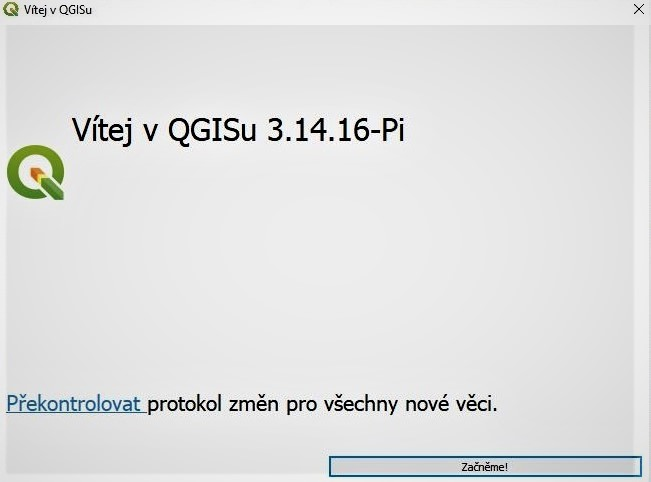
\includegraphics[width=8cm]{../pictures/qgis_startup_window.JPG} 
\caption[Welcome to QGIS 3.14 window]{Welcome to QGIS 3.14 window (Source: Personal collection)}
\label{fig:qgis_startup_window}
\end{center}
\end{figure}

\noindent After this introduction, we are redirected to the main software window (Fig. \ref{fig:qgis_first_window})  informing about community events and significant improvements that have taken place. Here we can choose an empty project template or we may open sample datasets (North Carolina, South Dakota, Alaska) provided along with instalation.

In QGIS 3, we distinguish between the layer's and project's CRS. It is worth mentioning that QGIS supports about 2700 known coordinate systems, whose definitions are stored in the SQLite database installed together with QGIS. The empty project has always global default projection EPSG: 4326 - WGS 84.

\vspace{0.3cm}
\begin{figure}[hbt!] 
\begin{center}
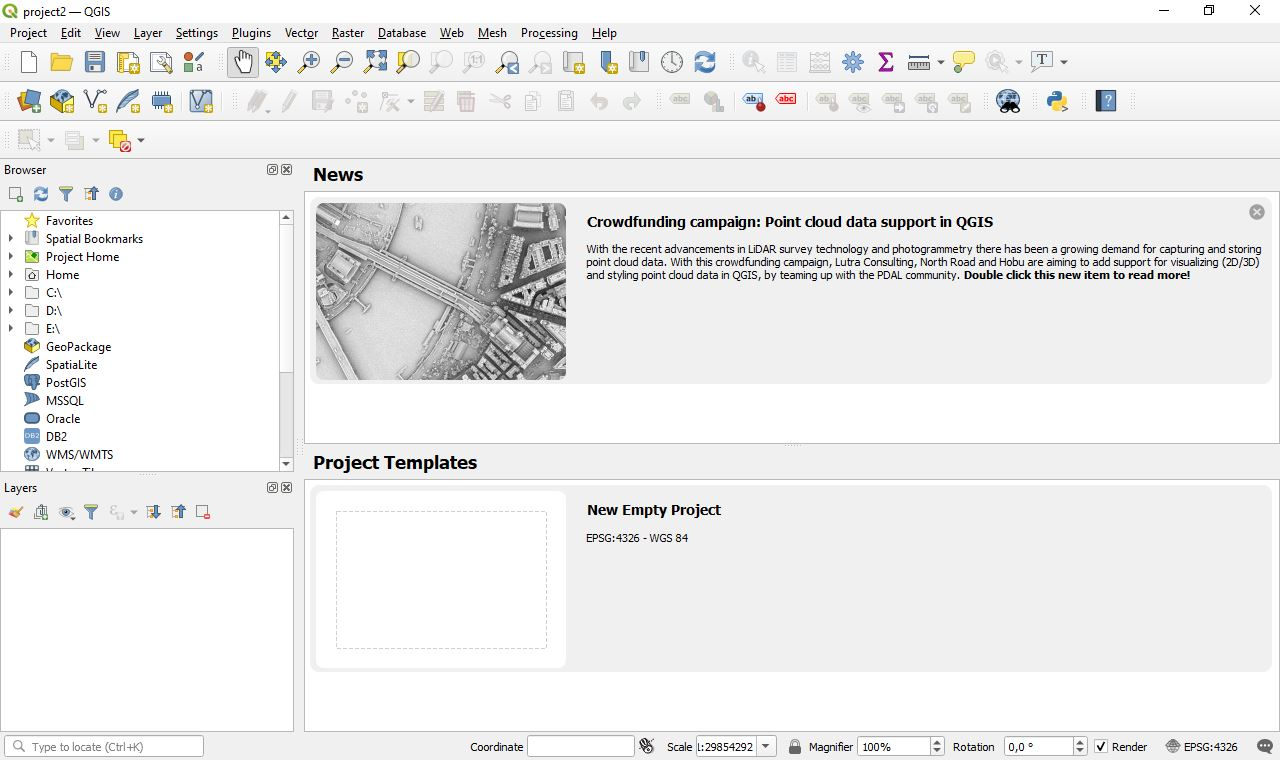
\includegraphics[width=17cm]{../pictures/qgis_first_window.JPG} 
\caption[The main software window after first opening QGIS 3.14]{The main software window after first opening QGIS 3.14 (Source: Personal collection)}
\label{fig:qgis_first_window}
\end{center}
\end{figure}

\noindent In QGIS, On-the-fly transformation is enabled by default, meaning that whenever you use layers with different coordinate systems QGIS transparently reprojects them to the project CRS. When importing the first layer (in this case US tracts in ESRI: 102003 system), the dialog box shown in Fig. \ref{fig:qgis_transformation} specifies what type of transformation to perform when changing the project CRS. These Datum transformations are then listed in Project Properties - CRS settings (Fig. \ref{fig:qgis_trans}). It is important to note that the first layer added defines the coordinate system of the project. In our case, it was changed to the US Contiguous Albers Equal Area Conic system. In the dialog \ref{fig:qgis_trans} we can set the Predefined coordinate system, which is related to the project, not to the layer.

Whenever a more accurate transformation is available, but is not currently usable, QGIS 3 shows an informative warning message (see Fig. \ref{fig:qgis_warning_window}) advising to use more accurate transformation. Those messages appear quite often in a variety of situations, which can definitely help new as well as experienced QGIS users.

\begin{figure}[hbt!] 
\begin{center}

\includegraphics[width=17cm]{../pictures/qgis_warning_window.JPG} 
\caption[Informative warning message  in QGIS 3.14]{Informative warning message  in QGIS 3.14 (Source: Personal collection)}
\label{fig:qgis_warning_window}
\end{center}
\end{figure}

\begin{figure}[hbt!] 
\begin{center}
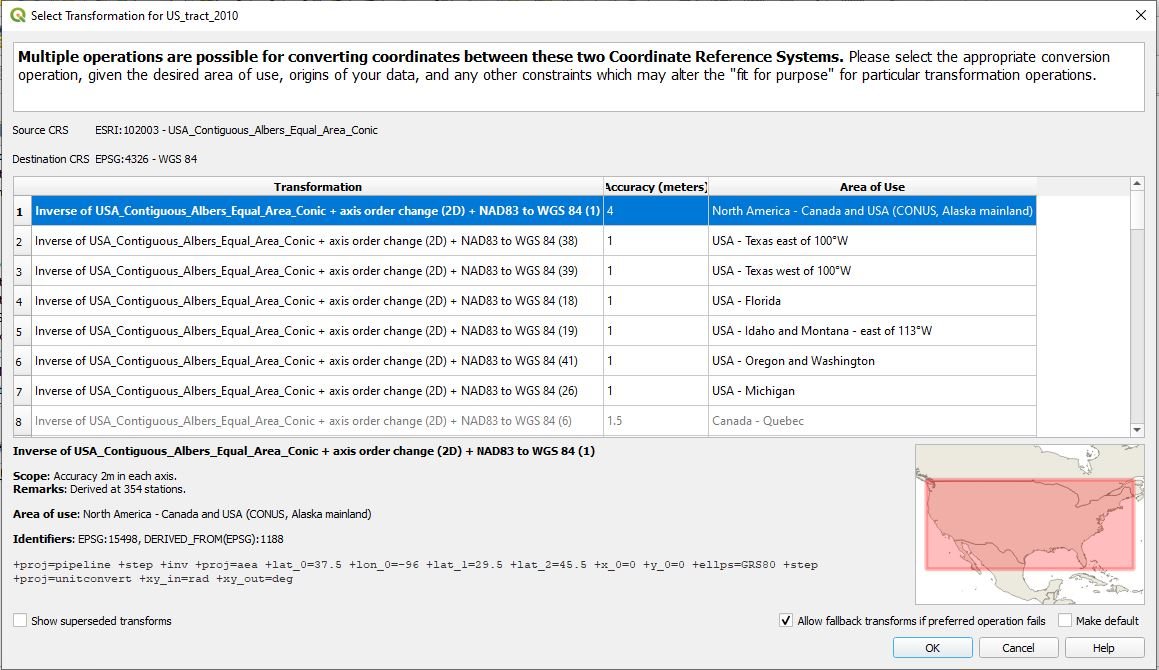
\includegraphics[width=14cm]{../pictures/qgis_transformation.JPG} 
\caption[Select the type of transformation in QGIS 3.14]{Select the type of transformation in QGIS 3.14 (Source: Personal collection)}
\label{fig:qgis_transformation}
\end{center}
\end{figure}

\begin{figure}[hbt!] 
\begin{center}
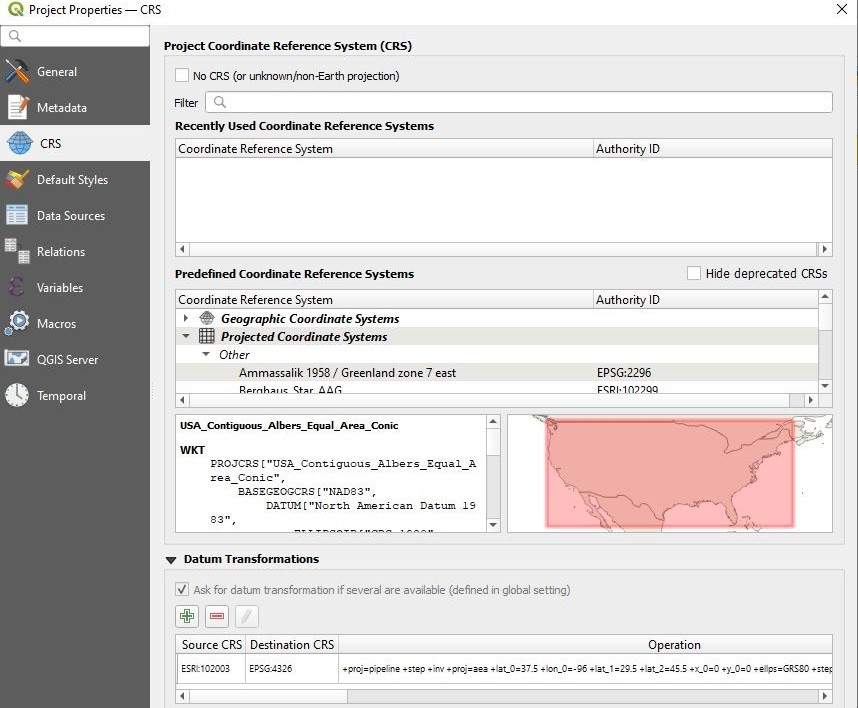
\includegraphics[width=14cm]{../pictures/qgis_trans.JPG} 
\caption[Predefined CRS and Datum Transformations in QGIS 3.14]{Predefined CRS and Datum Transformations in QGIS 3.14 (Source: Personal collection)}
\label{fig:qgis_trans}
\end{center}
\end{figure}


\newpage
\vspace*{-1cm} 
\bigskip

\noindent \textbf {gvSIG 2.5.0}

\noindent Here we will describe the startup mechanism of another open-source software created under the OSGeo organization. gvSIG can work with common vector and raster data, integrates files and databases as well as remote data through OGC standards. It is developed in Java and, like QGIS, includes a plugin system which allows to easily extend the software capabilities and develop tailor-made solutions.

Software is designed very simply. It does not have a startup window, nor does it support any first-time mode. When started, an empty map window will open. The work is saved in a project with the extension * .qvsproj, which can then be started through the associated icon. If we do not start the software using the project's association icon, it is reopened by default with a blank map. Adding layers is also intuitive. It is possible to add multiple layers in different coordinate systems, the software recognizes the EPSG codes. The data still retains its original coordinate system, however, map layers are rendered in the WGS 84 (EPSG:4326) using On the fly transformation, see Fig. \ref{fig:gvSIG_coords}.

\vspace{0.3cm}
\begin{figure}[hbt!] 
\begin{center}
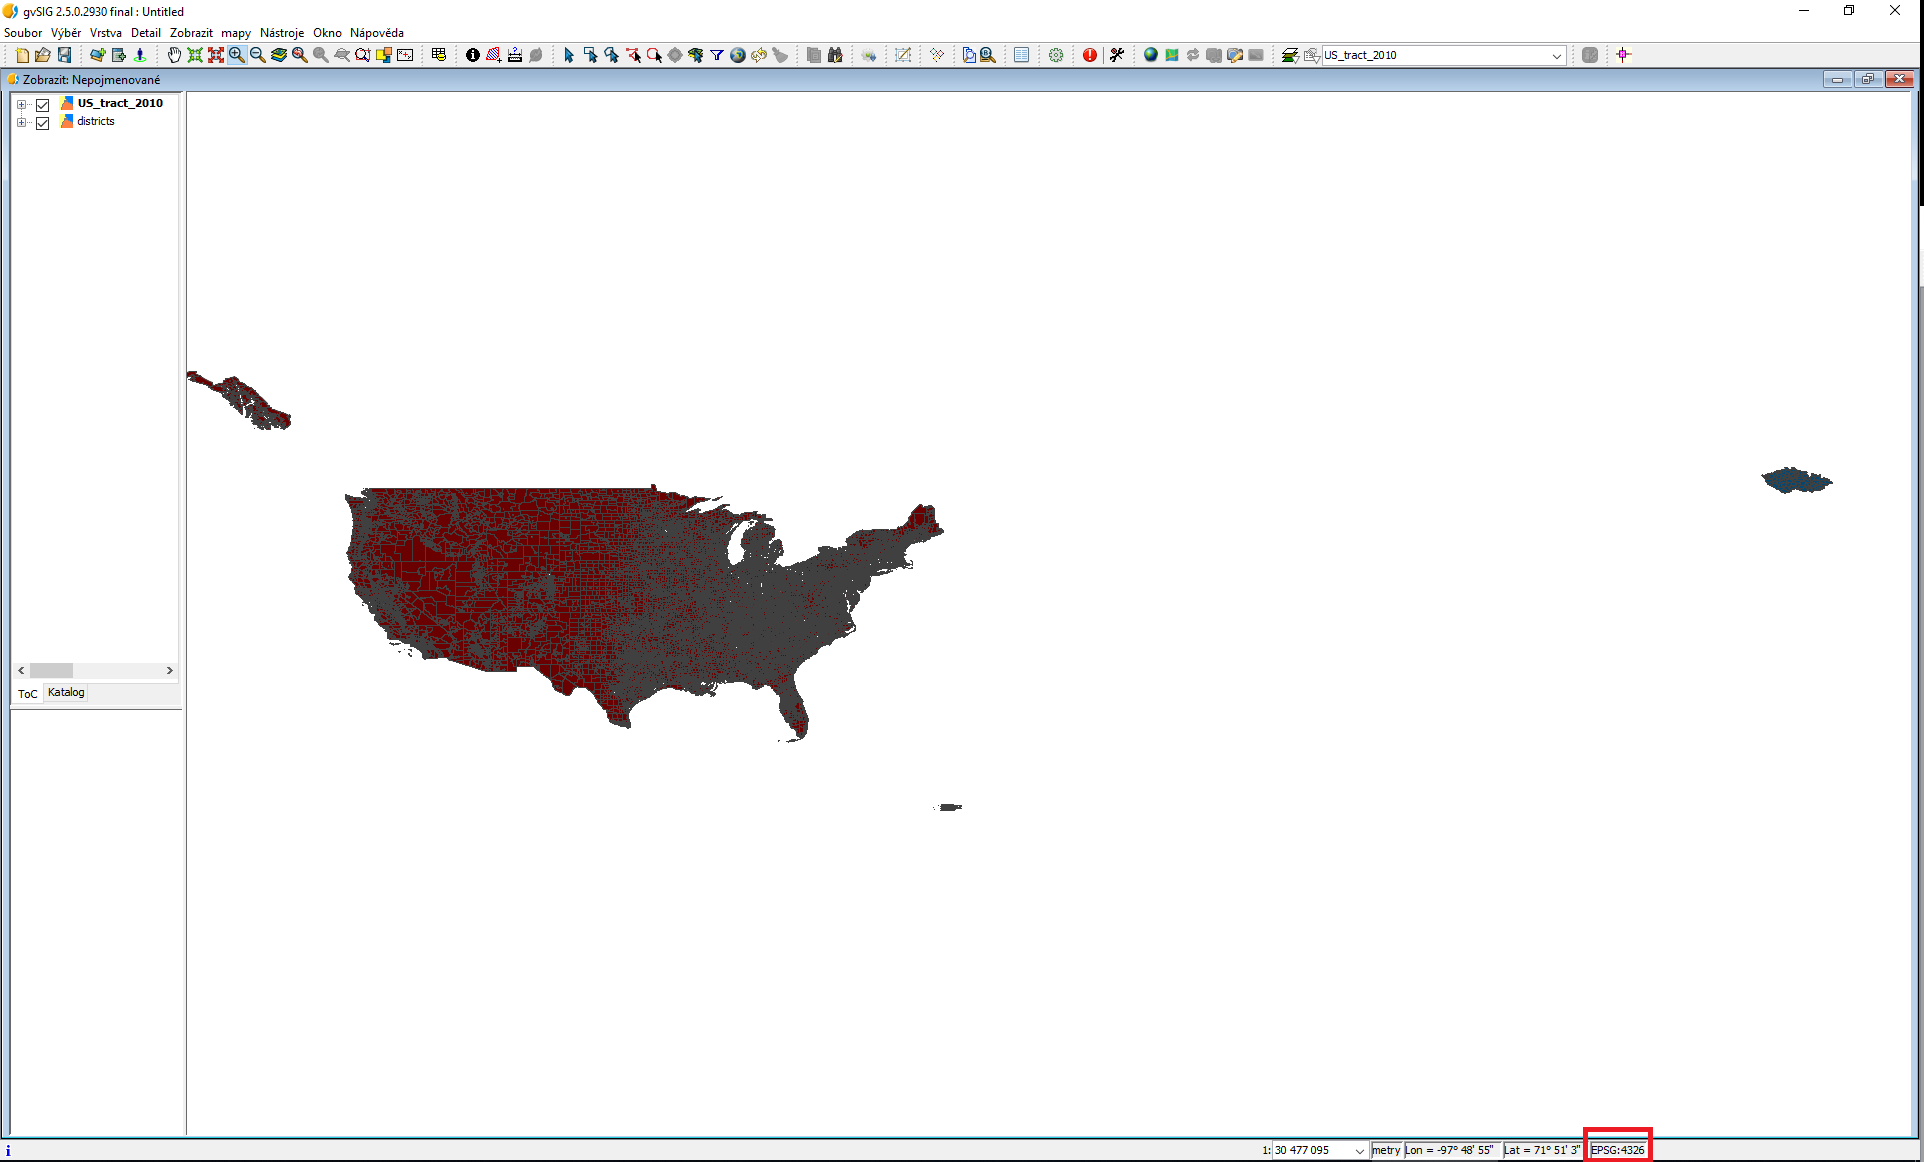
\includegraphics[width=17cm]{../pictures/gvSIG_coords.PNG} 
\caption[Correct display of layers with different coordinate system in gvSIG 2.5.0]{Correct display of layers with different coordinate system in gvSIG 2.5.0 (Source: Personal collection)}
\label{fig:gvSIG_coords}
\end{center}
\end{figure}

\newpage
\vspace*{-1cm} 
\bigskip
\noindent \textbf {ILWIS 3.3 (Integrated Land and Water Information System)}

\noindent The strong point of this system developed at University of Twente in the Netherlands has always been remote sensing and hydrological flow operations.

The software starts without a startup window and does not have features enhancing first-time user experience. On the left there is a section with several tabs: Operation-Tree, Navigator and Finder. ILWIS seems to be very similar to GRASS GIS. Operation-Tree and Finder are defacto the Modules tab in GRASS divided into two sub-tabs.  The data is similarly to GRASS stored in the home directory here called Data, which is taken as the default when importing or creating data. The content of this folder is in special formats that ILWIS understands, see Figure \ref{fig:ilwis_uvodni_okno}. 

The navigator has a tree structure like the GRASS Data Catalog and represents the entire directory structure, not just a home Data directory. ILWIS does not have its own native file to save the projects or workspaces.

\vspace{0.3cm}
\begin{figure}[hbt!] 
\begin{center}
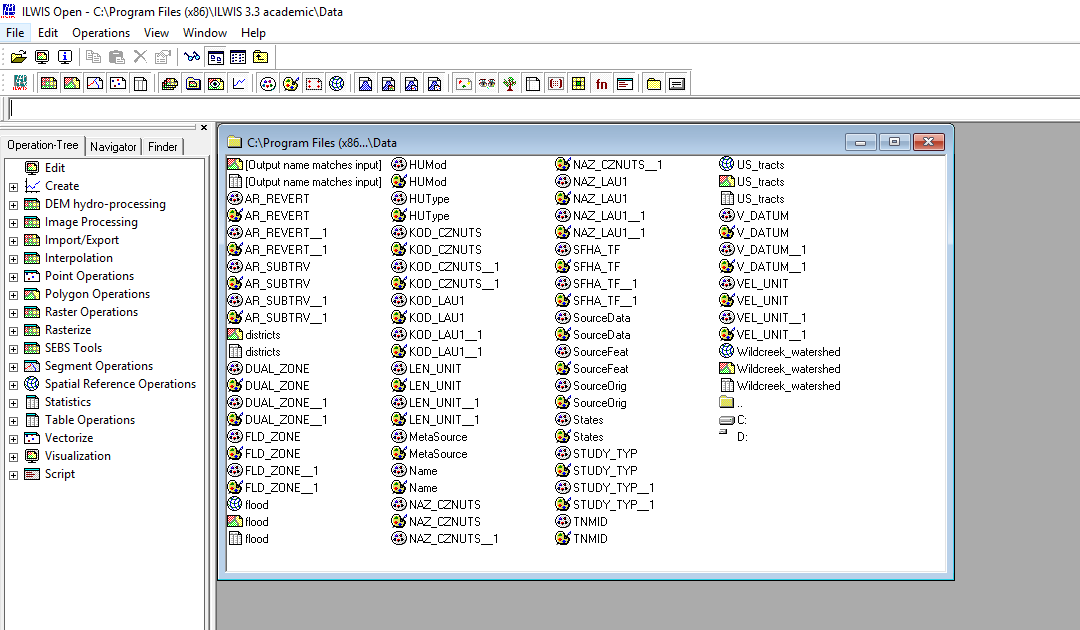
\includegraphics[width=17cm]{../pictures/ilwis_uvodni_okno.png} 
\caption[The main software window after reopening ILWIS 3.3]{The main software window after reopening ILWIS 3.3 (Source: Personal collection)}
\label{fig:ilwis_uvodni_okno}
\end{center}
\end{figure}

\noindent The display of layers with different coordinate system is tested as well. Importing data in the form of a shapefile is somewhat unintuitive here. If we want to perform an import we might go to the Operation-Tree $->$ Import/Export $->$ Import Map, however we encounter the problem that the software does not know the shapefile format. Therefore, the second option can be found in the top bar File $->$ Import. Here we select the ESRI shapefile and it is necessary to expand the default output so that the imported file is saved as an ILWIS object with the * .ioc extension. If we do not do this, only the tables will be imported, no maps.

It is interesting how the software approaches coordinate systems. When importing the layer called districts, the S-JTSK Krovak East North system is converted to the Unknown. In case of US tracts, the US Contiguous Albers Equal Area Conic system is converted to the LatLon system. Therefore, the software does not carry information about a specific coordinate system, it only cares about boundaries of the map. When displaying multiple layers with different coordinate systems in one map window, no On the fly transformation is performed. The system gets confused and the added layer is not displayed even after clicking on the ''Zoom to Layer'' function. There is no need to save the software, after opening it reflects the current state of the Data folder.

\vspace{0.3cm}
\begin{figure}[hbt!] 
\begin{center}
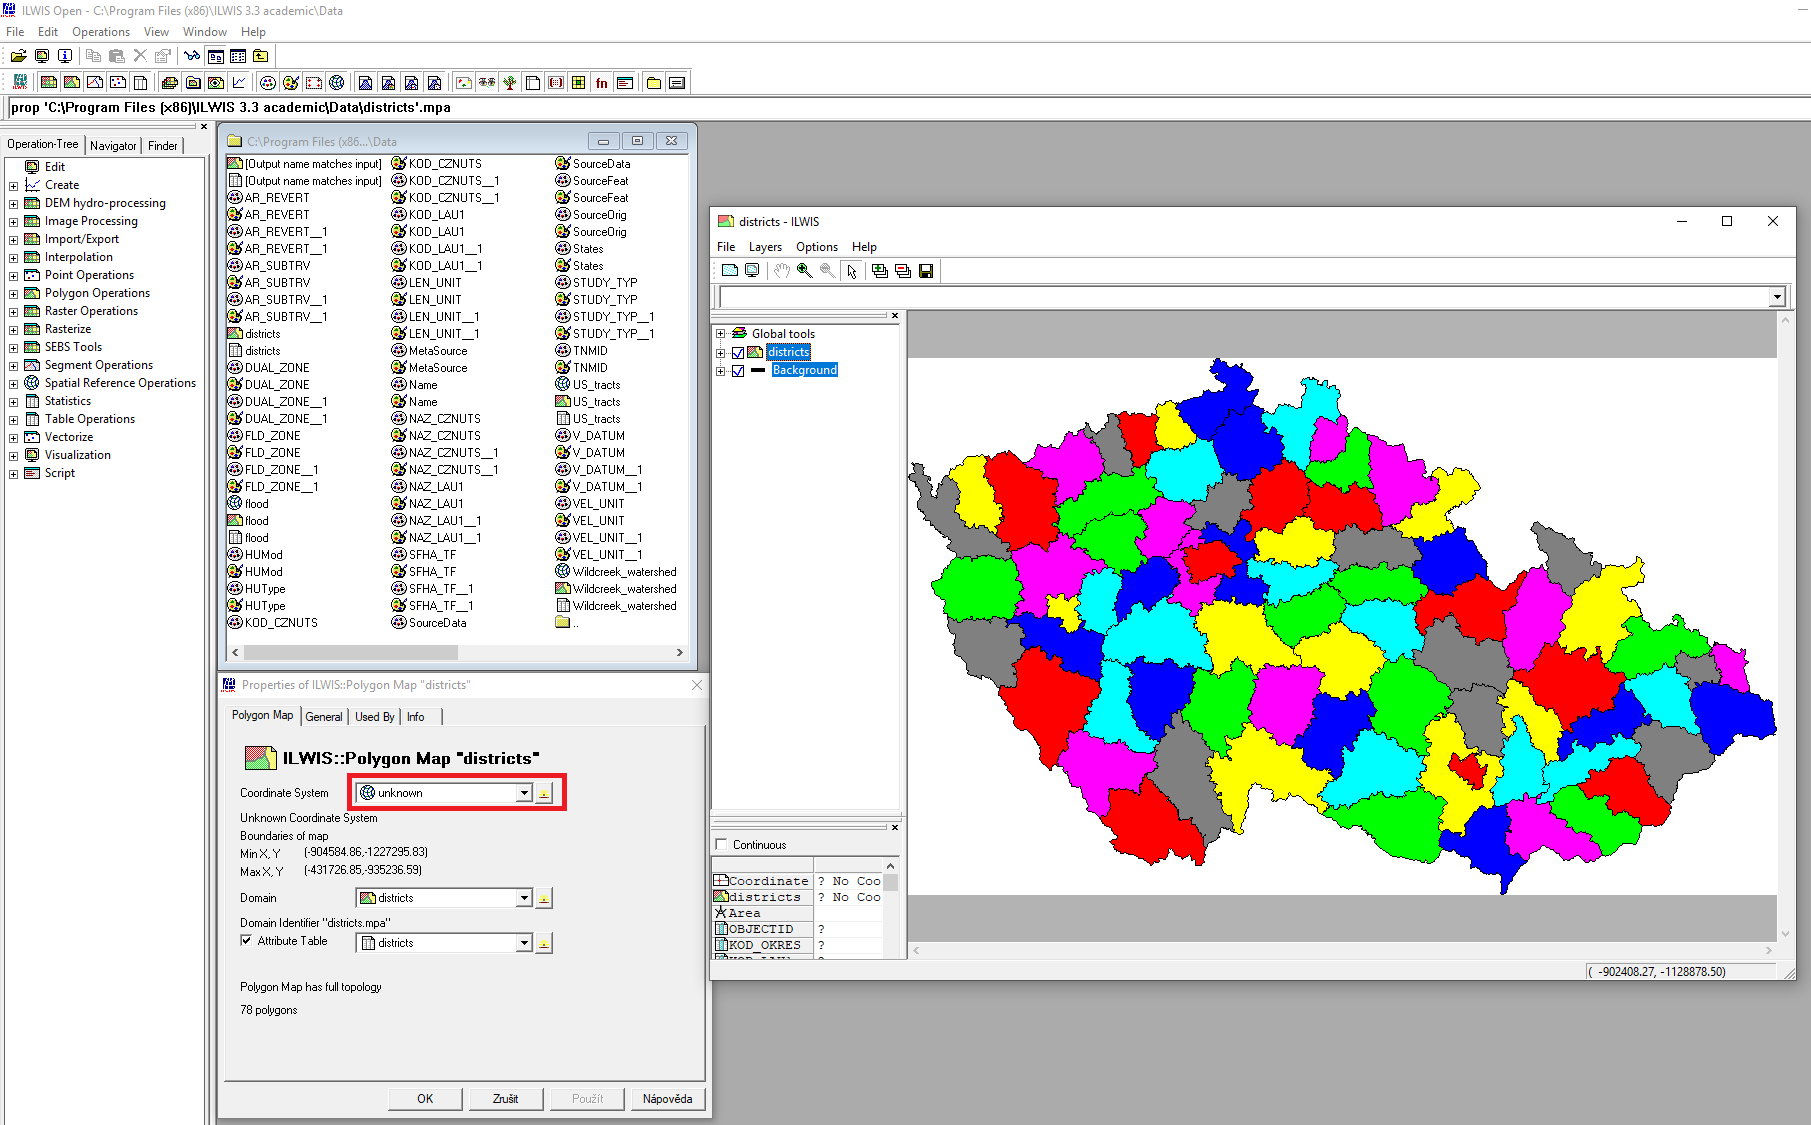
\includegraphics[width=17cm]{../pictures/ilwis_pridani_mapy.png} 
\caption[Unknown coordinate system properties of district layer in ILWIS 3.3]{Unknown coordinate system properties of district layer in ILWIS 3.3 (Source: Personal collection)}
\label{fig:ilwis_pridani_mapy}
\end{center}
\end{figure}

\bigskip

\noindent \textbf {SAGA GIS 2.3 (System for Automated Geoscientific Analyses)}

\noindent SAGA GIS is a Free Open Source Software (FOSS) offering a comprehensive, growing set of higher-level geoscientific methods. It is one of the most favorite software for remote sensing needs because of its rich library grid, imagery and terrain processing modules.

This software is blank the first time it is run. On the left there is a window with the Tools, Data and Maps tabs, which are similar to the Modules, Data, Layers tabs in GRASS GIS 7.8. The Data and Maps tabs are further divided into the Tree and Thumbnails subtabs. The tree is divided according to the shapes of geometric objects (point, line, polygon ...). 

The idea is different from GRASS GIS. The directory structure of added layers is always displayed for the current layer in the lower left window of Data Sources in the File System tab. So we do not have a specific folder in which we work from the beginning. We can add layers to the tree structure and the whole project will be created only when we save the settings to a SAGA GIS project file.

In the Maps tab, multiple layers can be displayed on top of each other or a new map map window can be created for each layer, which is a default option. However, there is no On the fly transformation. It means that layers with different coordinate systems may be displayed at the level of one map.  As we can see in Figure \ref{fig:saga_gis_cele}, the Czech Republic appears next to the American continent, as the system assumes adding layers with the same coordinate system to the map.

After the second start of SAGA GIS, a small selection dialog box will appear. We can run a blank page, the latest software state, or the last running projects sorted from newest to oldest (Figure \ref{fig:saga_startup}).

\vspace{0.3cm}
\begin{figure}[hbt!] 
\begin{center}
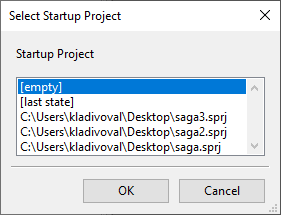
\includegraphics[width=6cm]{../pictures/saga_startup.png} 
\caption[Saga GIS 2.3 startup dialog]{Saga GIS 2.3 startup dialog (Source: Personal collection)}
\label{fig:saga_startup}
\end{center}
\end{figure}

\vspace*{-1cm} 
\subsubsection{Summary}
\label{subsec:startup_concepts_summary}

The summary corresponding to the questions asked at the beginning of this chapter is contained in the Figures \ref{fig:commercial_software} and \ref{fig:open-source_software}. In the cross-section of all selected GIS software, we can notice that the data hierarchy is quite different. The truth is that two world-famous representatives of GIS software - ArcGIS Pro and QGIS 3 -  have similar data organization into projects. However, in the data hierarchy of the other two commercial software GeoMedia and MapInfo, the term `` project '' does not appear at all. 

\newpage
\begin{figure}[hbt!] 
\begin{center}
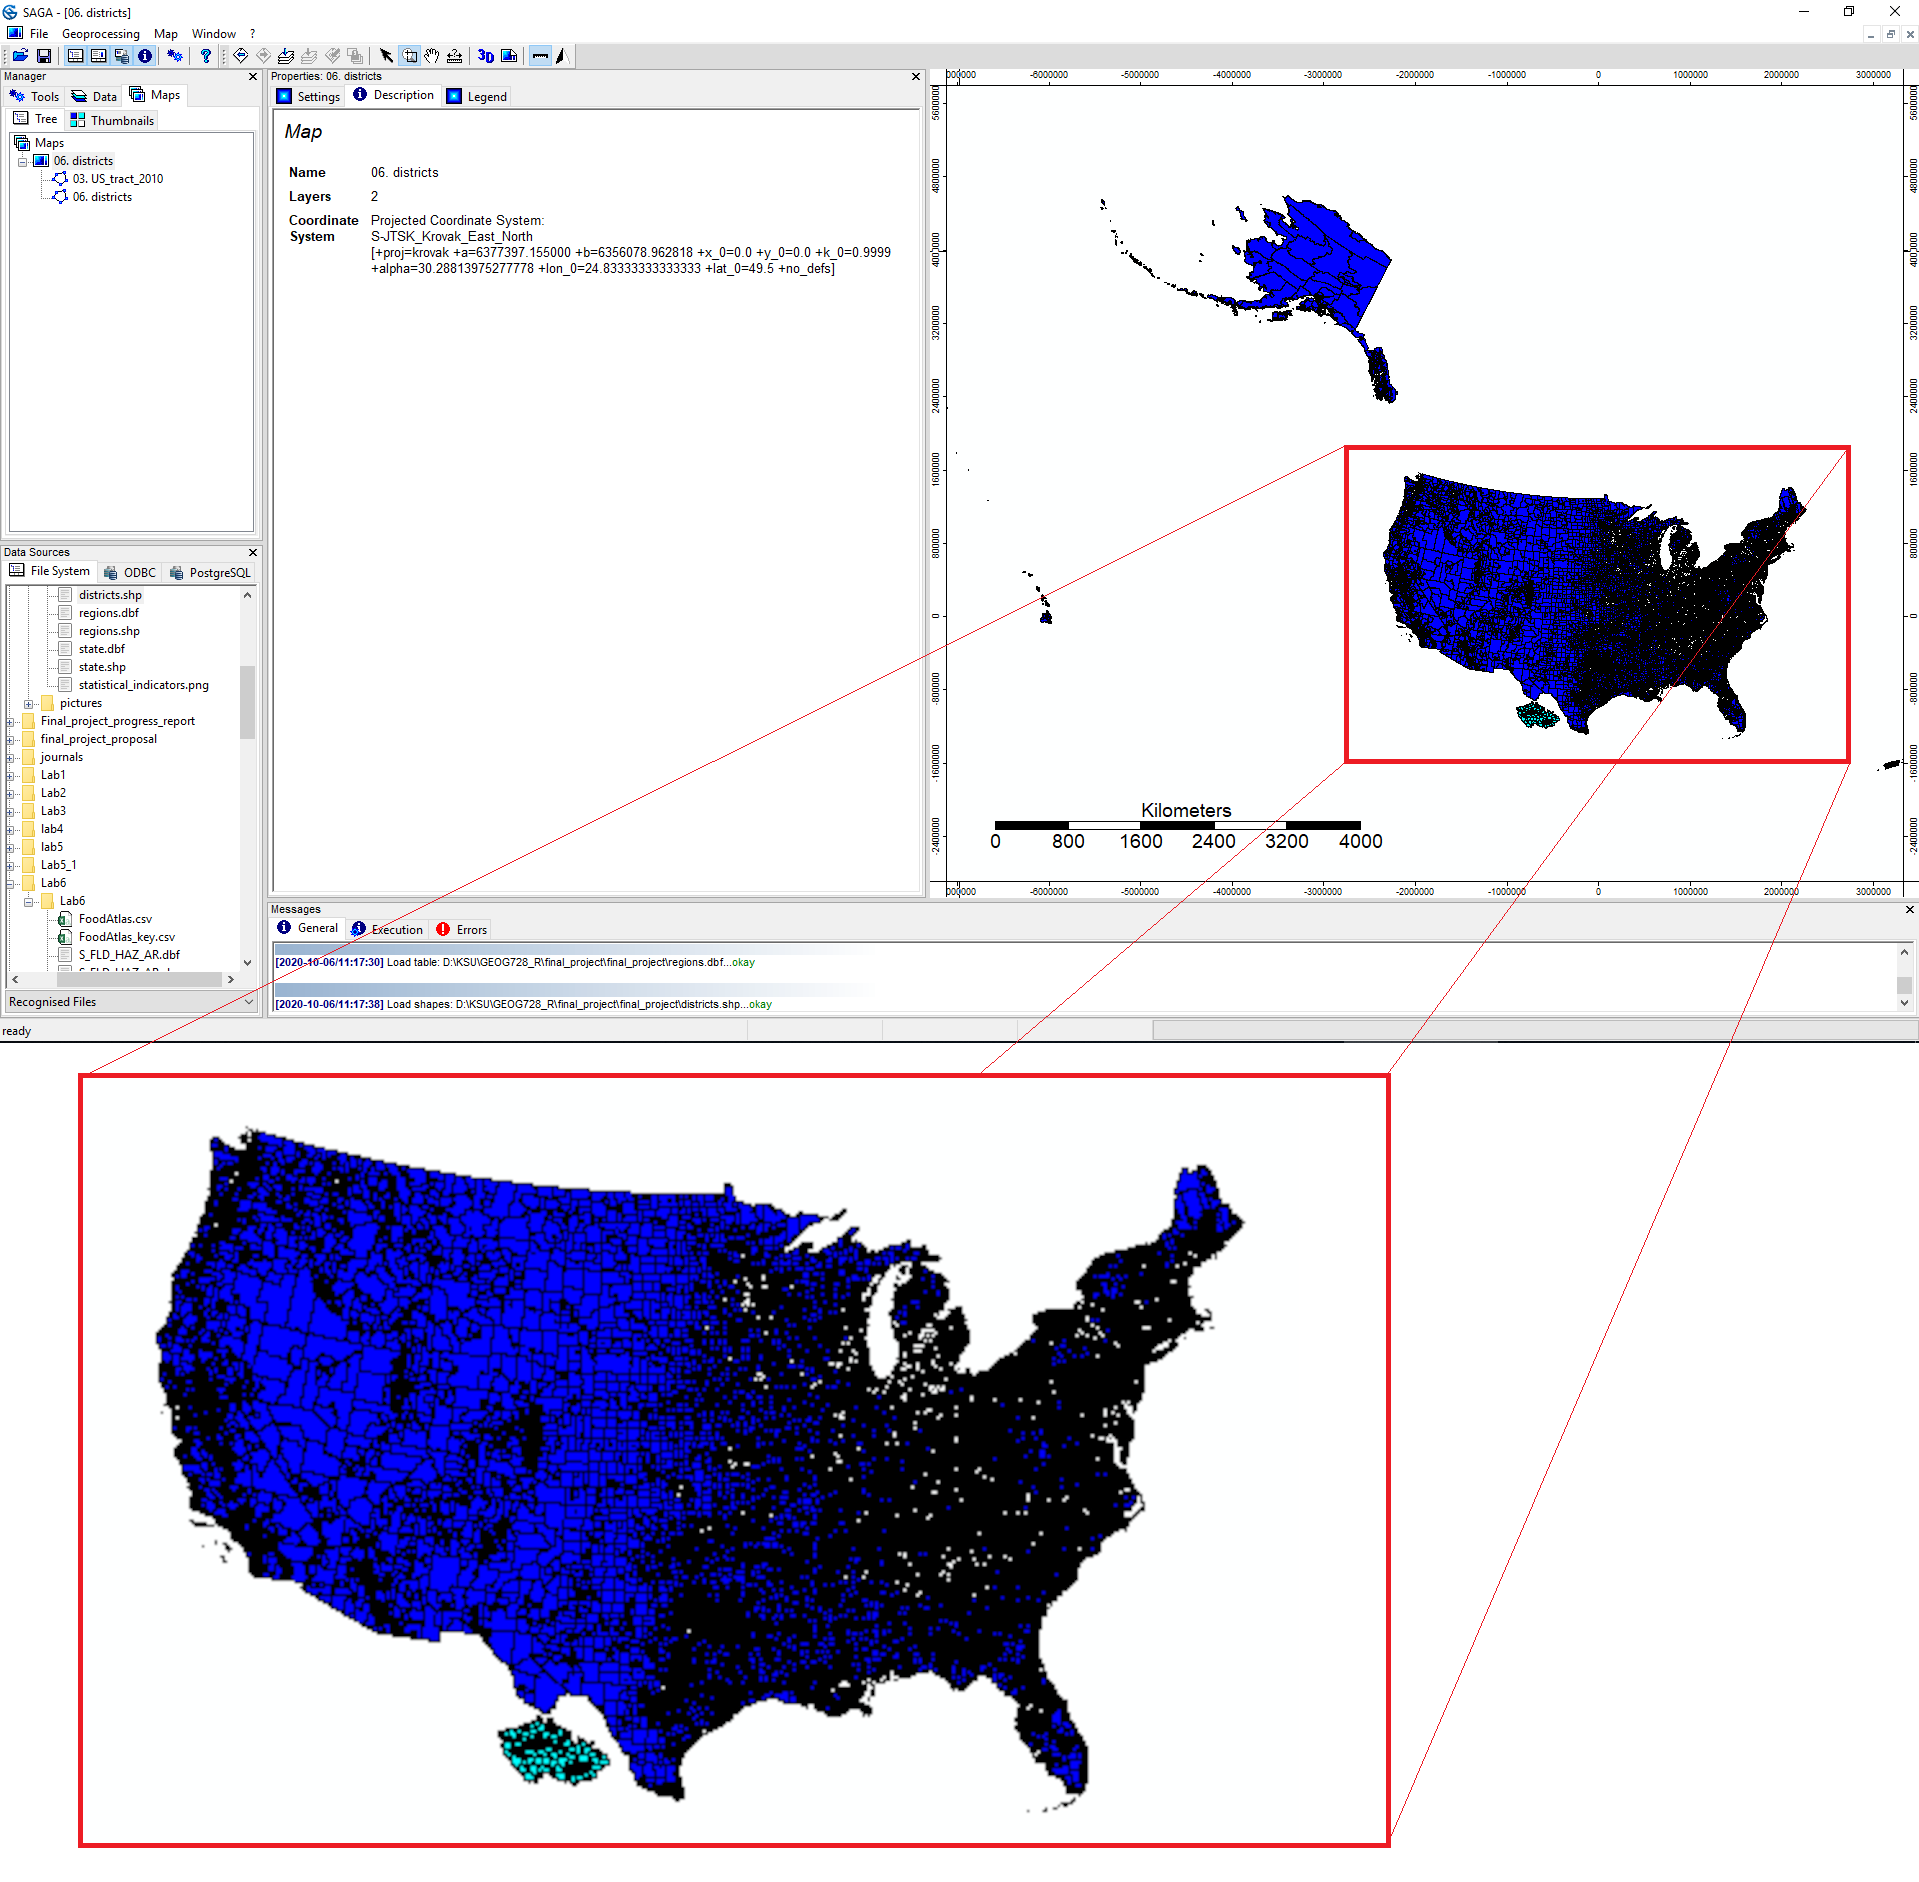
\includegraphics[width=17cm]{../pictures/saga_gis_cele.png} 
\caption[Incorrect display of layers with different coordinate system in SAGA GIS 2.3]{Incorrect display of layers with different coordinate system in SAGA GIS 2.3 (Source: Personal collection)}
\label{fig:saga_gis_cele}
\end{center}
\end{figure}

\noindent It is therefore good to realize that we may consider this name as a standard for data organization, especially for open-source software, but after looking at commercial software we find out that data organization across software is surprisingly different not only from a technical point of view, but also in terms of different names.

Startup screens appear in some form in all selected commercial software. For GeoMedia, it is a small dialog box whose purpose is purely organizational - choose the GeoWorkspace you will work in. For ArcGIS Pro and MapInfo, startup screens play a more important role. It tries to impress users with both modern design and the services they offer. Similarly, QGIS tries to make contact with the user from the beginning - it refers to news and displays Info Bars (see Fig. \ref{fig:qgis_warning_window}).

It is surprising how much of a difference there can be between commercial GIS software in terms of efforts to enhance the first-time user experience. With the GeoMedia software, the author did not manage to record any effort at all, on the contrary, MapInfo is very generous to its user from the very beginning and uses modern technologies in startup screen, such as videos on YouTube. Despite the fact that in some of selected software there is a certain effort to better interact with the initial user, none of them contains any first run wizard incorporated directly in the main software window (as offered by Zoner Photo Studio X, see the next chapter \ref{sec:other_software}). But this is not necessarily wrong. Whether any help at all makes sense and will not be rather counterproductive strongly depends on the complexity of data organization in a particular software. For example, with gvSIG software, there is no startup screen or any other helpful explanation, although it can be assumed that the new user will find his way around without any problems. GeoMedia also lacks any interactive features, however, as data organization is more complex to understand, it is likely to be much more inconvenient start for users.

As known, GRASS GIS went a different way from the beginning. Not only in data organization. The difference between GRASS and other GIS software goes far beyond the startup mechanism or data organization. Let's remember the unique Unix philosophy, where the software consists of a collection of small applications called modules, or the ability to call these modules from the command line. It is therefore interesting to note that the comparison of GRASS GIS with other GIS software does not provide significant inspiration for other implementations associated with the improvement of the startup mechanism, which requires (and probably deserves) a completely unique solution whose roots were laid already in the summer of 2020 by GSoC implementations. However, the comparison offers an interesting look at this topic, which is not talked about much, but certainly has a big impact on the whole software. The evidence may be, after all,  user complaints about the problematic startup screen in versions before GSoC.

We do not have to look for inspiration only in GIS software. How the software interacts with the first-time user is a completely general thing that plays a role in all types of software. In the next chapter, the author highlights several interesting cases of startup mechanisms involving user interaction. These are software that the author either uses herself or received a tip in the Quesion 4 from the second part of the survey number 1.

\vspace{0.3cm}
\begin{figure}[hbt!] 
\begin{center}
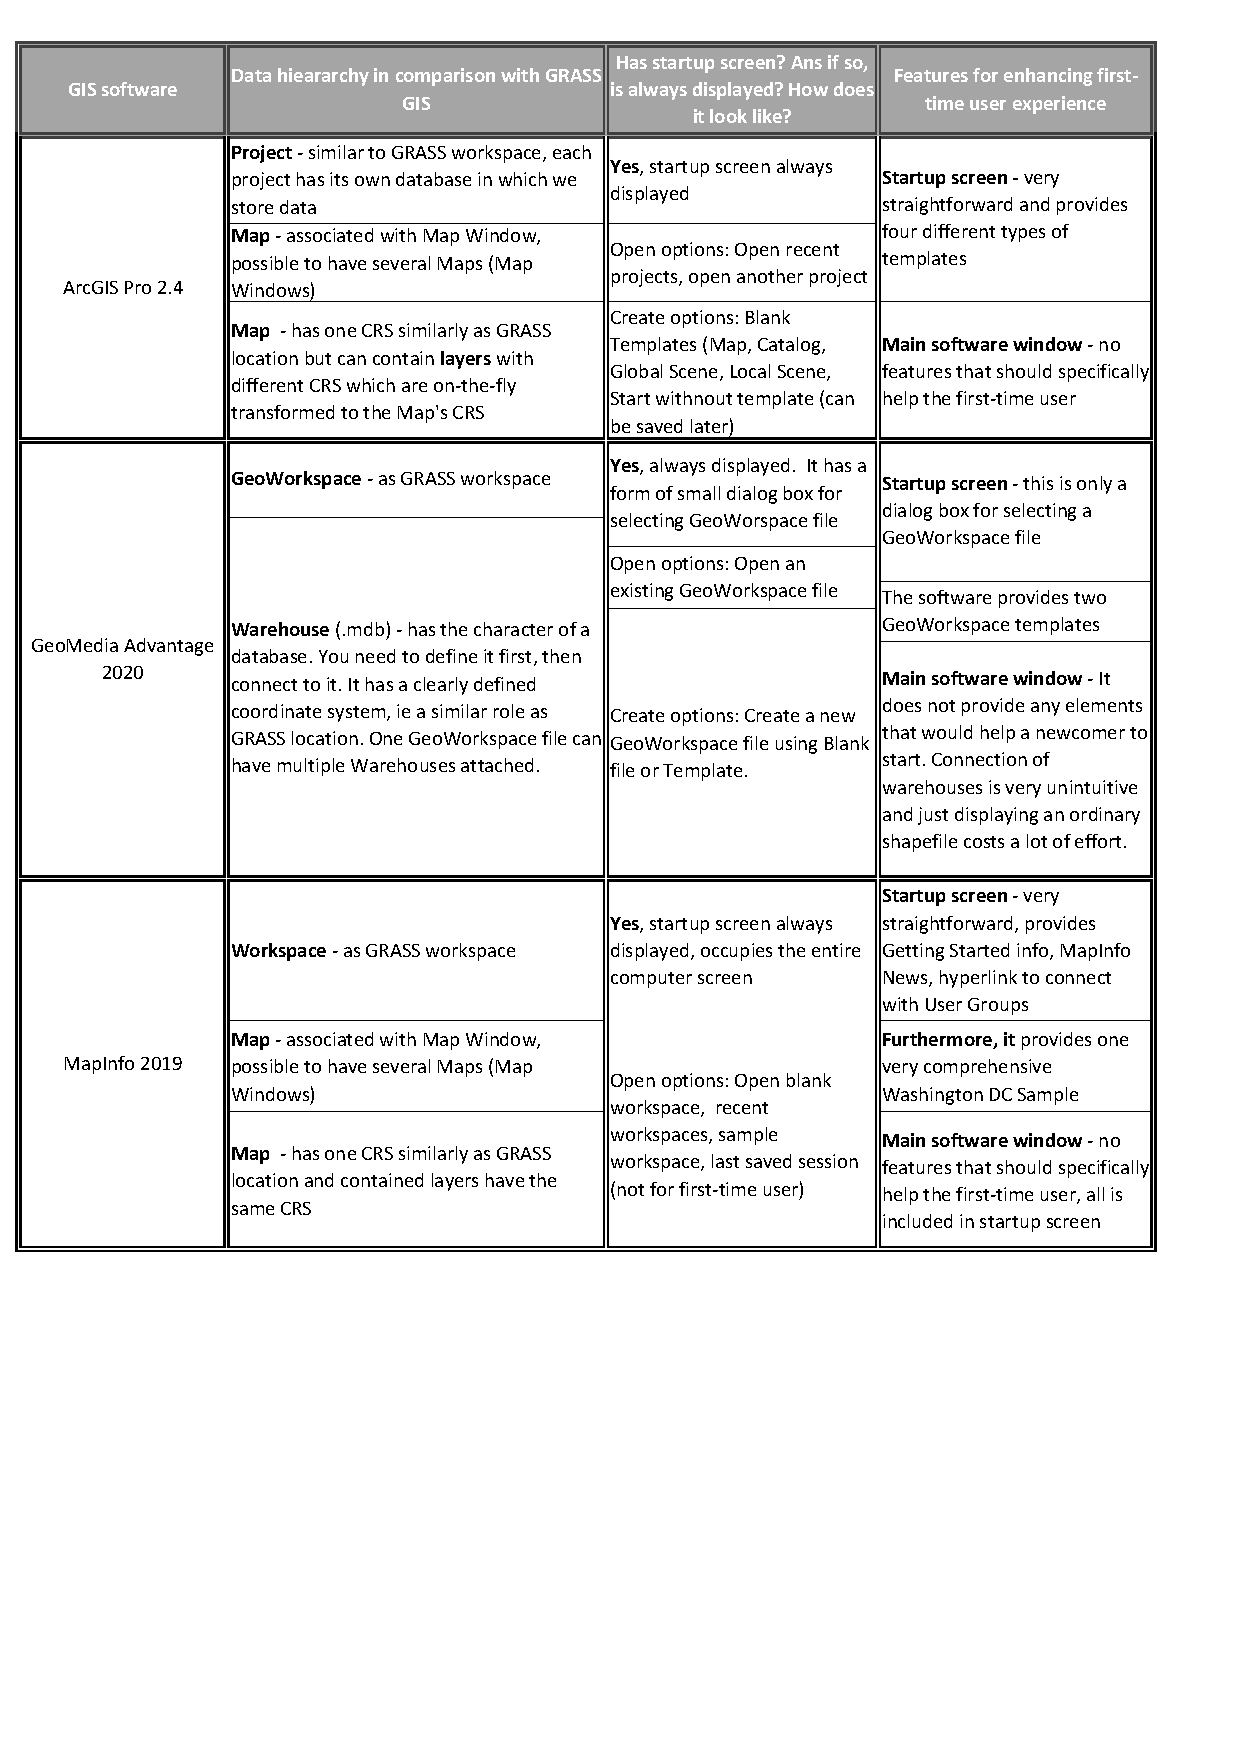
\includegraphics[width=15cm]{../pictures/commercial_software.pdf}
\caption[Analysis of selected commercial software]{Analysis of selected commercial software (Source: Personal collection)}
\label{fig:commercial_software}
\end{center}
\end{figure}

\vspace{0.3cm}
\begin{figure}[hbt!] 
\begin{center}
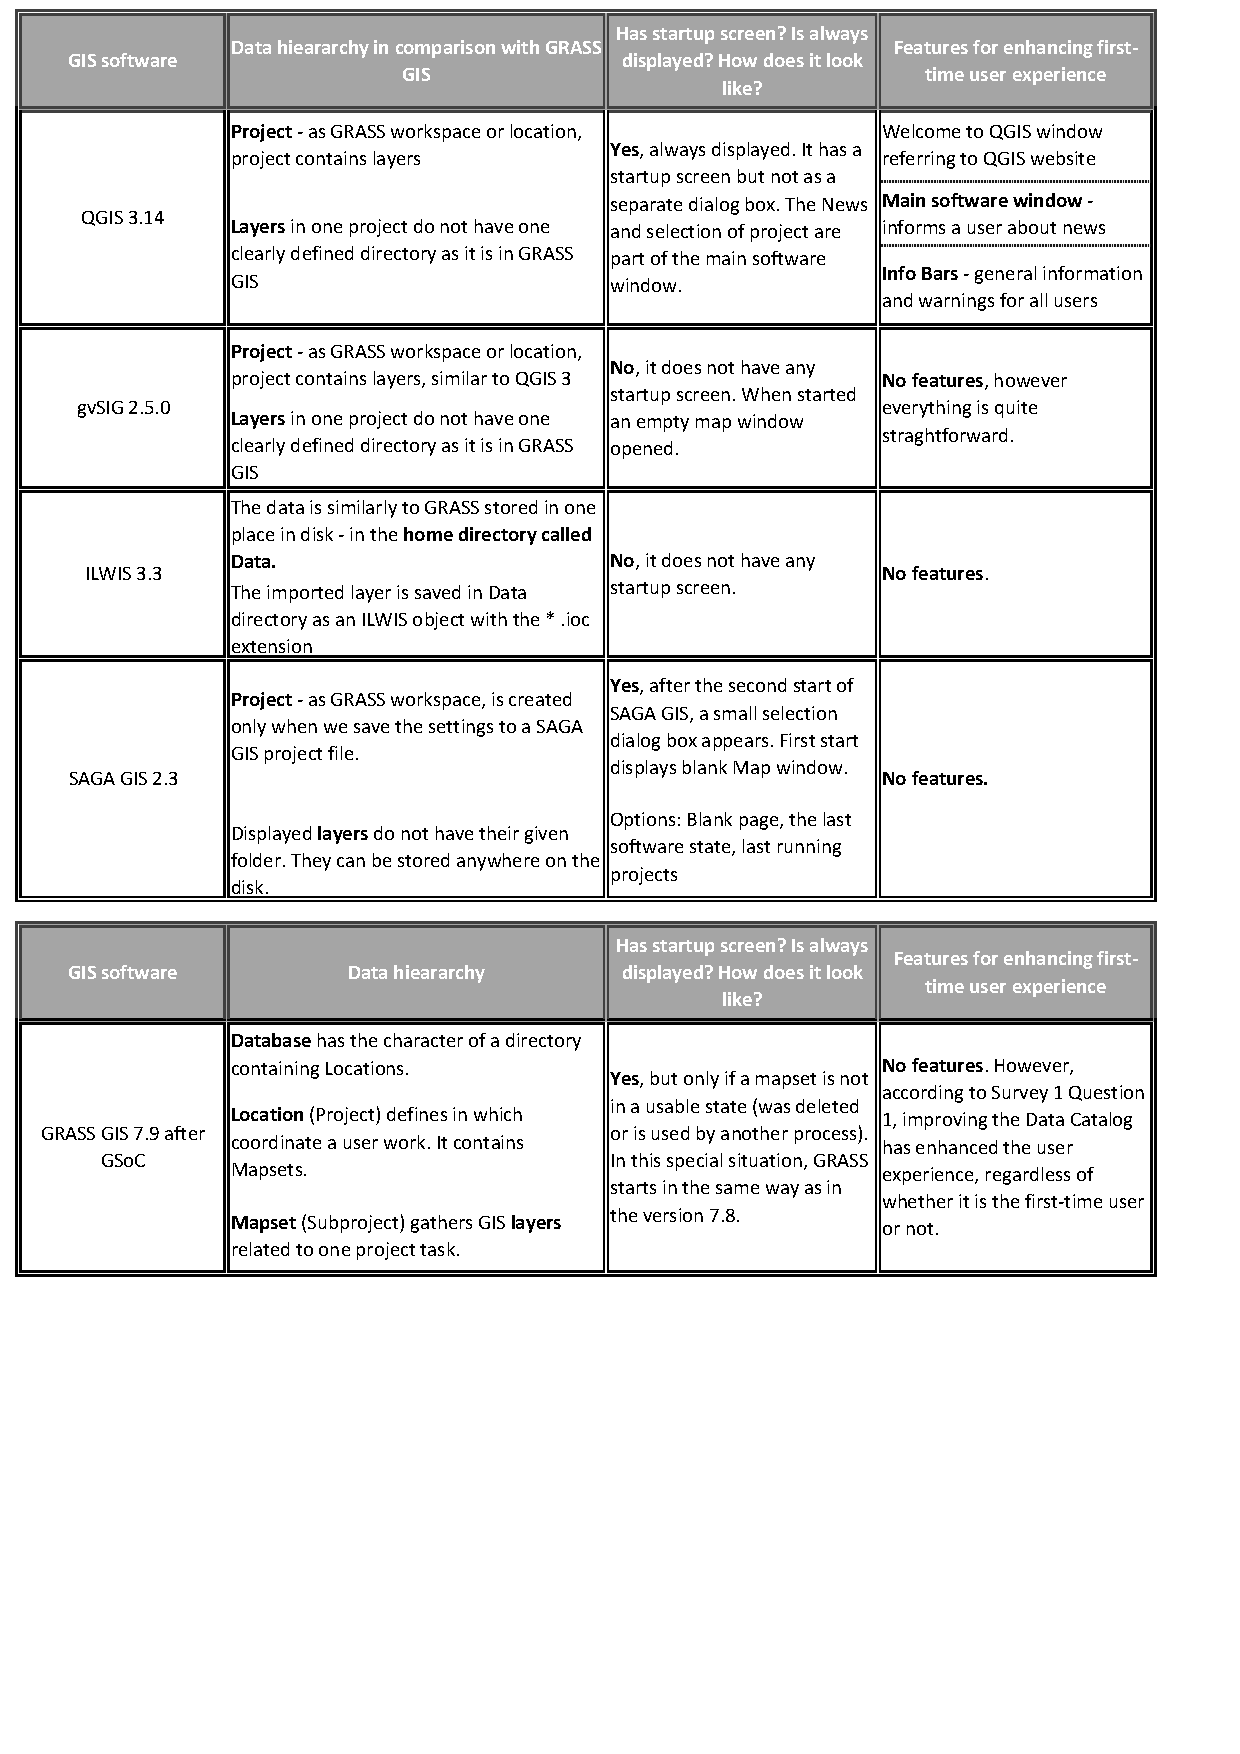
\includegraphics[width=15cm]{../pictures/open-source_software.pdf} 
\caption[Analysis of selected open-source software and GRASS GIS]{Analysis of selected open-source software and GRASS GIS (Source: Personal collection)}
\label{fig:open-source_software}
\end{center}
\end{figure}


\newpage
\vspace*{-1cm} 
\subsection{Interesting solutions from other software}
\label{sec:other_software}

\noindent \textit{\color{red}Dokončit!}

\noindent \textbf{Zoner Photo Studio X} \\

\noindent After the initial login and launching the main software window, a short first run wizard will appear and can be skipped. The guide consists of four parts. The first section introduces the main tabs on the left side of the software window called the Navigator and also explains the Catalog tab, which provides quick access to photos. The following are two pages of a guide describing photo thumbnails and zooming. The last page of the wizard lists the right toolbar and the three individual modules - Manager, Develop and Editor. The main software components described in the wizard are always marked with a blue frame and the individual information windows are assigned to a particular part by arrows. The wizard is not only at the beginning, but also when using the above-mentioned modules for the first time.

Images are managed in the Catalog, which has a tree structure. We edit the image, save it, and if we turn off the Zoner software and run it a second time, it starts up in the last opened file. If the last used file is deleted, the software is launched in the Manager tab in the last opened folder, where another image can be selected for editing or we can simply click to another folder and open or create another image. There is a native image format of Zoner Photo Studio X with extension * .zps, however, firstly, traditional formats such as * .jpg, * .png, * .tif, * .gif etc. are offered to us.

\vspace{0.3cm}
\begin{figure}[hbt!] 
\begin{center}
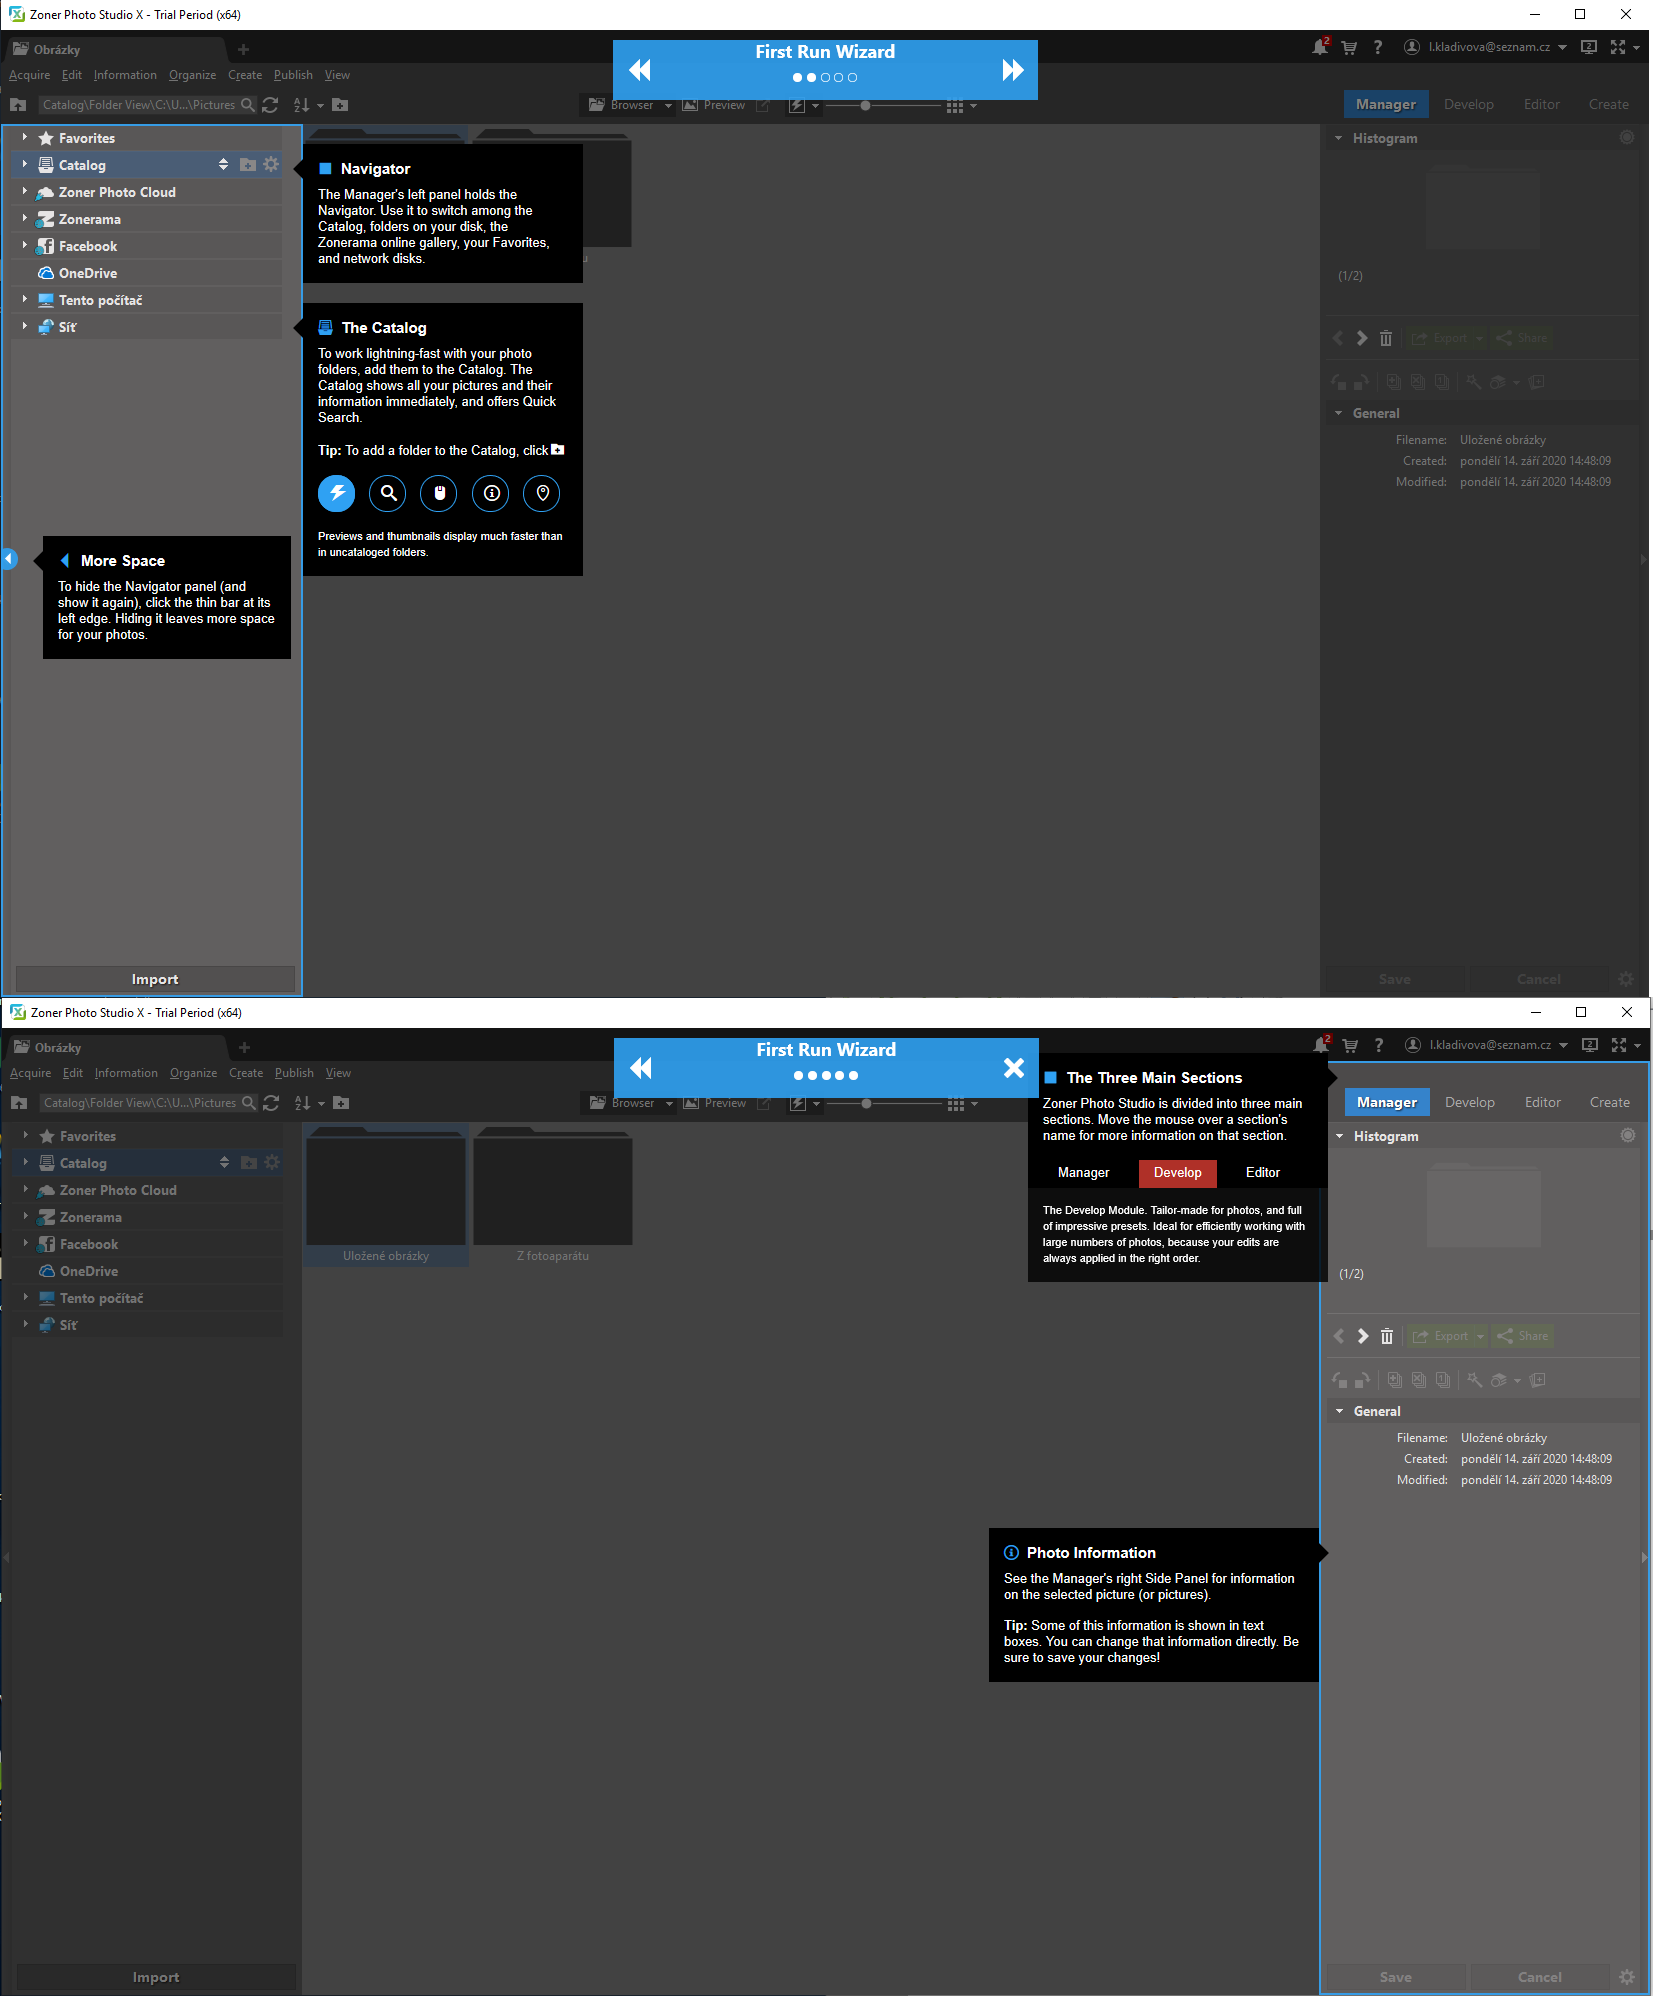
\includegraphics[width=15cm]{../pictures/zoner.png} 
\caption[First run wizard in Zoner Photo Studio X]{First run wizard in Zoner Photo Studio X}
\label{fig:zoner}
\end{center}
\end{figure}

\newpage
\vspace*{-1cm}
\subsection{Summary}


\newpage
\vspace*{-1cm}
\fancyhead[RE, RO]{\fancyplain{}{\small \sl{Usability testing methods}}}
\section{Usability testing methods}
\label{sec:usability_testing}


\noindent As Ana Amélia describes in her work [], the concept of usability is related to the field of Human-Computer-Interaction (HCI). Here we can find several definitions of what usability means. In the case of websites and software applications, usability refers to whether or not users can achieve specific goals with efficiency, effectiveness and satisfaction (Marcie Dishman). Booth (1989) mentions four aspects of usability testing: usefulness, effectinevess (ease fo use), learnability, and attitude.

As explained by https://www.hotjar.com/usability-testing/methods/, the main goal of usability testing is to test and validate the product hypothesis and specific design decisions using the end-user perspective. We can come across various options for dividing usability testing methods. The most recently used division, for example, at https://www.hotjar.com/usability-testing/methods/, https://usabilitygeek.com/remote-usability-testing-best-practices/ is as follows:

\begin{itemize}
\item	Moderated vs. unmoderated
\item	Remote vs. in person
\item	Explorative vs. assessment vs. comparative
\end{itemize}

\noindent A moderated testing is done with direct supervision. It investigates the reasoning behind user behaviour which allows a researcher to dig deeper into any pain points and usability issues. To test participants, answer their queries, and ask follow-up questions takes about 1 – 2 hours, and average number of participant is 3 – 5 (https://www.playbookux.com/10-popular-usability-testing-methods/). 

Conversely, an unmoderated test is not supervised. The participant is usually in their own home using their own devices to test the software usability. The problem is that an average tester might not understand the complexities of a product which can consequently cause the testing in a different way than was originally intended. It takes about 20 minutes and average number of participant is 5- 10 (https://www.playbookux.com/10-popular-usability-testing-methods/).

In-person testing provides very valuable data since researchers can also watch and analyze participants’ emotions. 
Remote testing are done over the internet or by phone and doesn’t go as deep into a participant’s reasoning. However, it allows a research to test large numbers of people in different geographical areas using fewer resources.

\noindent Explorative tests are open-ended, participant are asked to give opinions, think about new features. Assessment research tests a user's interaction with the product and how well they are able to use it.  It's used to evaluate the product's general functionality. Comparative research methods involve asking users to choose which of two solutions they would prefer.

\noindent User testing methods are very nicely captured on the following picture \ref{fig:usability_testing_methods}:

\vspace{0.3cm}
\begin{figure}[hbt!] 
\begin{center}
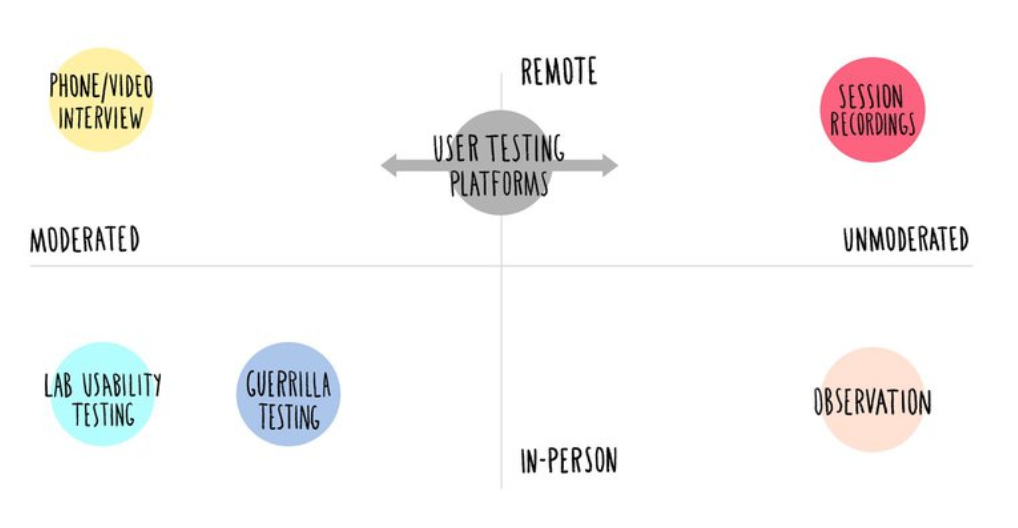
\includegraphics[width=17cm]{../pictures/usability_testing_methods.png} 
\caption[Usability testing methods]{Usability testing methods (source: https://www.hotjar.com/usability-testing/methods/)}
\label{fig:usability_testing_methods}
\end{center}
\end{figure}

\noindent It is important to emphasize that usability testing, using an appropriate method, is a valuable investment in a software product.
 
\subsection{Moderated + in-person usability testing}
Those tests are the best  in terms of collecting depth, comprehensive information. 
\smallskip

\noindent \textbf {Guerrilla testing}

\noindent This is the simplest form of usability test best in the early stages of the product development process. The people are asked to perform a quick usability test (maximum 10 minutes), often in exchange for a small gift. Test subjects are chosen at random from a public place, so that they may have no history with a product. This is the reason why Guerrilla testing is not suitable for testing products that require having special skills.

\smallskip

\noindent \textbf {Lab usability testing}

\noindent This type of usability research usually takes place inside the controlled environment that is different from the user’s real environment. 
Lab usability testing works best if we need very comprehensive and detailed information about how the user works with the program and what problems they encounter. Participants perform tasks and the researcher monitors them and asks questions. It is important that the moderator is trained and able to help participants, but at the same time he should let them think and not tell them exactly what to do. The moderator should also be able to read human emotions. After testing, it is also crucial to discuss and analyze the specific problems the participants have faced.

\subsection{Moderated + remote usability testing}
Moderated and remote usability tests are performed via a computer or phone and require a trained moderator. They are good for picking from a wide range of participants while still taking advantage of a moderator's skills and ability to dive deep.

\smallskip

\noindent \textbf {Phone interviews}

\noindent In a phone usability test, a moderator verbally instructs participants to complete tasks on their computer and collects feedback while the user interaction is recorded remotely. This is a very good option to test users all over the world. 

\smallskip

\noindent \textbf {Card sorting}

\noindent Card sorting is the simple method which involves placing concepts or features on virtual cards and allowing participants to manipulate the cards into groups and categories. After they sort the cards, they explain their logic to a moderator. It is used for better organizing content and features in user interface.

\subsection {Unmoderated + in-person}
Unmoderated in-person tests offers many of the benefits of testing in a controlled atmosphere and reduces the possibility that a researcher could influence participants with their questions.

\smallskip

\noindent \textbf {Contextual inquiry}

\noindent Sometimes also called the Interview/Observation is the method especially suitable for obtaining information about the user's habits and preferences or to evaluate whether the user is satisfied with the product. The researcher first asks a series of questions about the experience with the product and then gives the user a task to work on independently. A research will not provide any opinions and can only interfere if the participant gets stuck on something. Otherwise a observer remains silent,  focuses mainly on the emotions and behavior of the user, and writes notes which will be then summarized in a detailed test report.

\smallskip

\noindent \textbf {Eye-tracking}

\noindent This special method allows scientists to observe the movements of the user's eyes using a special device located on the monitor, and to create heatmaps (where the user most often looked). The disadvantage of this method is that it requires a lab with special equipment and software.

\subsection{Unmoderated + remote usability testing}

Test participants are asked to complete tasks alone in their own environment using their own devices. It does lead to the natural participant's behaviour, however, this type of testing is less detailed. As a researcher can obtain larger amount of data, they could be able to have more confidence in a decision concerning their product. The main point is that a researcher need to ensure that every test instruction is clear. Unclear tasks can cause results missing right objectives. It is suitable for validation of particular question or hypothesis, however, it is not recommended to be used as a first usability testing method since it does not go deep into user’s thinking.

\smallskip

\noindent \textbf {Session recordings}

\noindent Session recordings use software to record the actions that anonymized people take on a website/software such as mouse clicks, movement, and scrolling. It helps to understand what content/features are the most interesting for the users as well as what interaction problems users encounter while they interact with the product.
\smallskip

\noindent \textbf {Online testing tools and platforms}

\noindent There are a variety of online testing tools that allow one to remotely observe user behavior. The most commonly used online testing tools are 5-second test and unmoderated card sorting.  In 5-second test, participants have five seconds to look at a screenshot of page before they answer the question. It is an easy way how to collect qualitative data about people’s first impressions and reactions. Card sorting, described above, can also be conducted in an unmoderated and remote manner if a researcher leaves out on the opportunity for follow-up questions.

\newpage
\vspace*{-1cm}
\fancyhead[RE, RO]{\fancyplain{}{\small \sl{Questionnaires}}}
\section{Questionnaires}
\label{sec:questionnaires}


\noindent As the reader of this work probably realized surveys (questionnaires) were not mentioned among unmoderated + remote usability testing. The reason is that questionnaires are not usually considered as usability testing because it does not require to directly test product functionality. However, in some literature [6 usability, Ana Amélia], questionnaires are also included in usability testing methods. In Ana Amélia's work, for example, the survey includes both - interview and questionnaire techniques. The questionnaire refers to a technique that can fall under the so-called expert/heuristic method, which works with experienced people who identify problems a less experienced user might encounter. As [6 usability] writes, questionnaires are not as numerically grounded and precise as other forms or testing, but they can provide important feedback from user group in a short time. They can take the form of specific questions about the software and its future development. 

Questionnaires must, above all, be effective. Therefore, in this new field very different from the field of programming, it was necessary to acquire new knowledge that will help avoid beginner's mistakes. How the surveys were conceived and what they would look like eventually crystallized by combining two different information flows.

The first flow is based on what type of questionnaire is usually used if we want to examine the software usability. For this purpose, we can use the widely used standard questionnaire known as the System Usability Scale (SUS). This questionnaire having 10 five-point items with alternating positive or negative tone was introduced by Brooke in 1996 [John Brooke]. The standard version is shown in Figure \ref{fig:sus}. The aim of this work is to obtain more detailed responses from GRASS users related to specific topic, so using this questionnaire alone does not make much sense in this work. However, the Slider questions (see \ref{sec:slider}) are technically realized similarly as in SUS - the interviewer does not evaluate questions but statements. It can often happen that the user would not use the queried functionality, but they assume that the others do, which results in a positive answer. Statements encourage the user to better express their own opinions.

The second source that inspired the author in composing the surveys was a user survey workshop within the All Things Open platform in which the author participated. The visited video conference \footnote{\url{https://2020.allthingsopen.org/sessions/user-experience-secrets-to-better-surveys-happier-users/}} led by professionals Dan Zola and Kerry Thompson from SWAY UX set out a few key rules for creating a questionnaire from which to get as much information as possible.

\vspace{0.3cm}
\begin{figure}[hbt!] 
\begin{center}
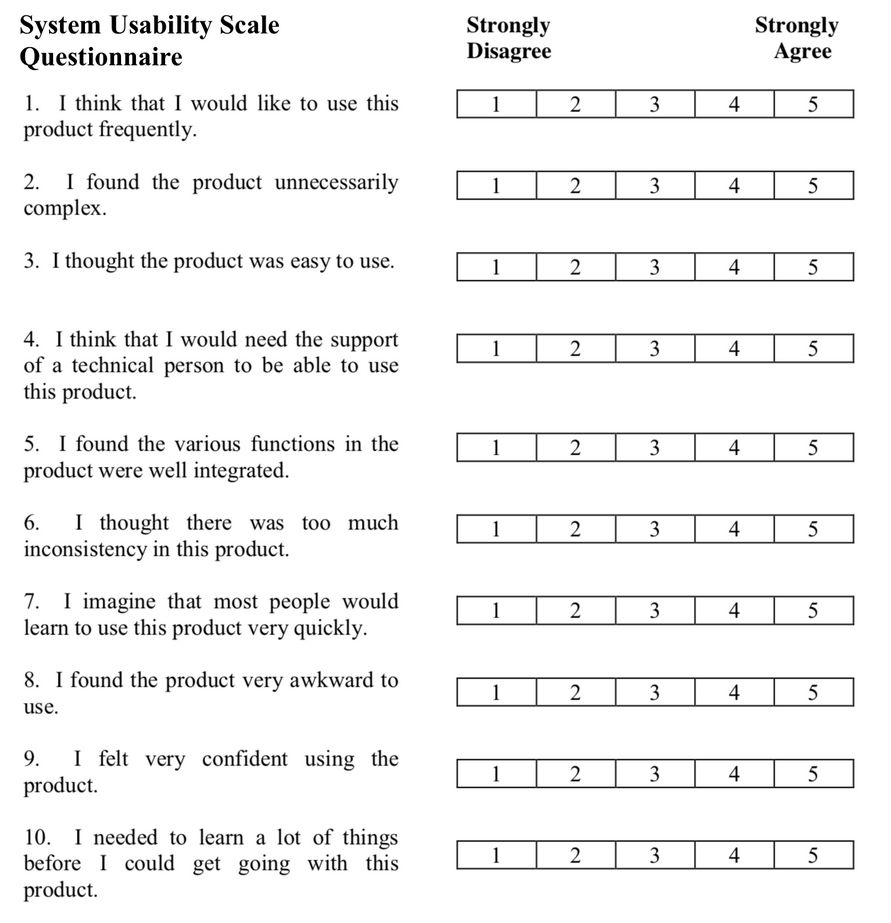
\includegraphics[width=14cm]{../pictures/sus.png} 
\caption[System Usability Scale Questionnaire (SUS) ]{System Usability Scale Questionnaire (SUS) (source: https://www.bentley.edu/centers/user-experience-center/what-every-client-should-know-about-sus-scores SUS - A quick and dirty usability scale John Brooke)}
\label{fig:sus}
\end{center}
\end{figure}

\newpage
\noindent According to the lecturers, the user survey helps with evaluation of customer safisfaction as well as understanding who are users and what are their pain points and priorities. It can be conducted not only at the start of the new project but basically at any time the survey administrator (developer) needs user input. 

In order to understand what makes up good questionnarre, it is first necessary to clarify what constitutes bad questionnarre. The workshop summarized the following 8 errors in particular:

\begin{itemize}
\item Too many questions (max 10 questions)
\item Convoluted questions
\item Answer choices that do not correspond with user's reasoning
\item Question that require long and comprehensive answers (if open-ended questions, always put them at the beginning)
\item Answers that could have more than one meaning
\item Answers that do not provide any information
\item Straight line answers
\item Vague answers (scale from 1-10, where an answer is 5)
\end{itemize}

\noindent The latter vague answers can occur in the case of answers with a rating scale. Although the authors of the workshop do not explicitly mention the SUS questionnaire, they strongly recommend avoiding the rating scale. The result could look similar to the following example in Fig. \ref{fig:blur_scale}. It is much more advantageous to use either binary answers (Yes / No) or rank specific features. 

\vspace{0.3cm}
\begin{figure}[hbt!] 
\begin{center}
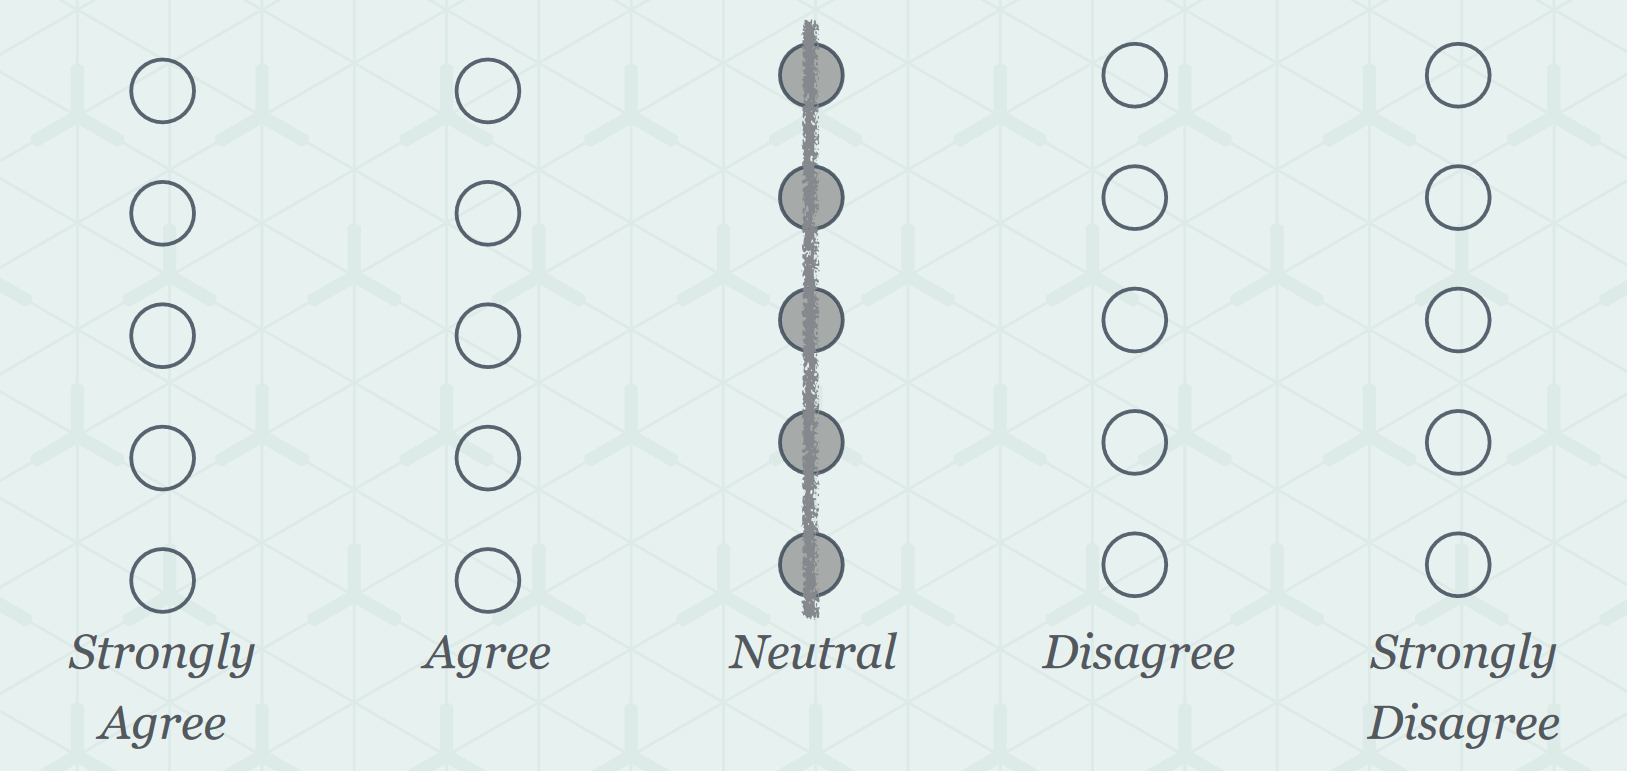
\includegraphics[width=12.5cm]{../pictures/blur_scale.png} 
\caption[Difficult interpretation of the rating scale answers]{Difficult interpretation of the rating scale answers (source: danzolakerrythompson)}
\label{fig:blur_scale}
\end{center}
\end{figure}

\noindent As mentioned at the beginning of the chapter, questionnaires are not usually considered as usability testing because it does not require to test product functionality.
However, it would be very challenging (if not impossible) in our work to ensure users having both versions of GRASS GIS (version 7.8 and version 7.9 after GSoC) and perform usability testing in forms of Lab usability testing or Contextual inquiry methods. Therefore, it was finally decided to use questionnaires as the main testing method.

\newpage
\vspace*{-1cm}
\subsection{Types of questions}

\noindent The author followed the advice to avoid rating scale questions. Instead, she used Slider and Ranking methods, which unfortunately are not offered by the free Google Forms service but only by the paid Survey Monkey (SM) service that was eventually used. The complete list of question types offered by the Survey Monkey platform can be seen in Figure \ref{fig:survey_monkey_options}. Those marked in green are used in surveys in this work. The following lines will shed light on the advantages of the types used and the procedure of processing them.

\vspace{0.3cm}
\begin{figure}[hbt!] 
\begin{center}
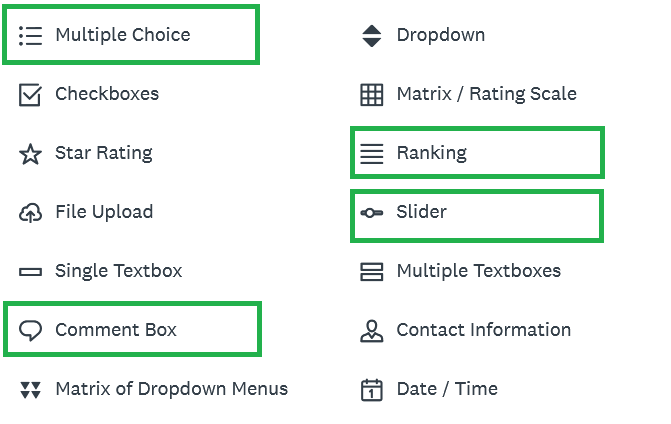
\includegraphics[width=10cm]{../pictures/survey_monkey_options.png} 
\caption[Survey Monkey answer types ]{Survey Monkey question types (source: https://www.surveymonkey.com)}
\label{fig:survey_monkey_options}
\end{center}
\end{figure}


\noindent \textbf {Slider}
\label{sec:slider}

\noindent This type of question, also called Visual Analog Scale (VAS), can be used instead of a rating scale. We let respondents rate an item or statement on a numerical scale by dragging an interactive slider. This method is visually more pleasant than the so-called Likert scale, which is the scale used in SUS. In addition, it best captures the true opinion and perception of users, as there is no limited LS 'discrete set of predetermined responses. Slider are, for example, widely used by healthcare professionals to determine their patient's pain. The pain does not have discrete jumps, but it is continuous, so it is appropriate to express it on a continuous scale from 0 to 100. As Matevž Pesek, Alja Isakovic concluded the Slider (they call it Stripe) increases the intuitiveness, simplicity and speed of answering the question. Therefore, this method is widely represented in the surveys conducted in this work. The form of the questions are inspired by the SUS questionnaire, in which users do not essentially evaluate the question, but try to express a degree of agreement with the opinion, which takes the form of a statement. A typical example of Slider question can be seen in Figure \ref{fig:slider_question}.

\vspace{0.3cm}
\begin{figure}[hbt!] 
\begin{center}
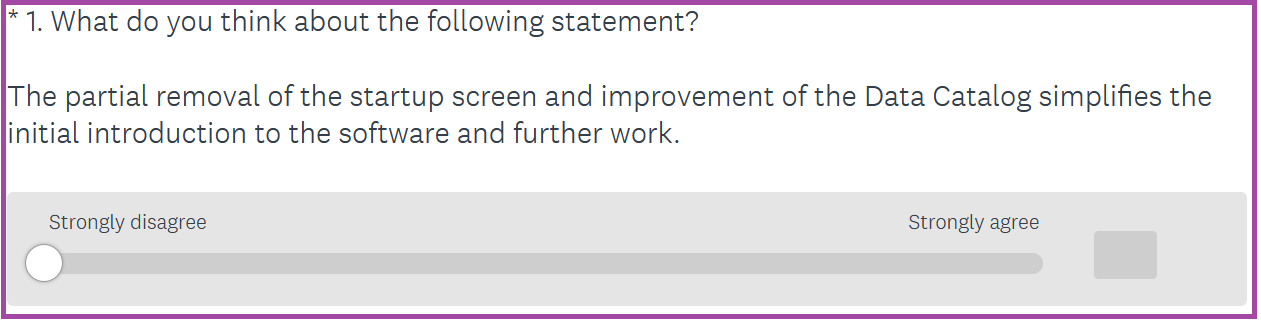
\includegraphics[width=16cm]{../pictures/slider_question.png} 
\caption[A typical example of a Slider question]{A typical example of a Slider question (Source: Personal collection)}
\label{fig:slider_question}
\end{center}
\end{figure}


\smallskip
\vspace*{-0.5cm}
\noindent \textbf {Ranking}

\noindent Ranking questions require the respondent to compare items to each other by placing them in order of preference. Although ranking answers usually have clear answers (the result cannot be an ambiguous answer somewhere in the middle as with the rating scale), it also has its disadvantages. It forces respondents to decide between items that they may perceive the same. It is also important for this type of question to follow the general principle that the order of the individual options is generated randomly. Otherwise, items earlier in the list may be more likely to be ranked highest. A typical example of Ranking question is provided in Figure \ref{fig:ranking_question}.

\vspace{0.3cm}
\begin{figure}[hbt!] 
\begin{center}
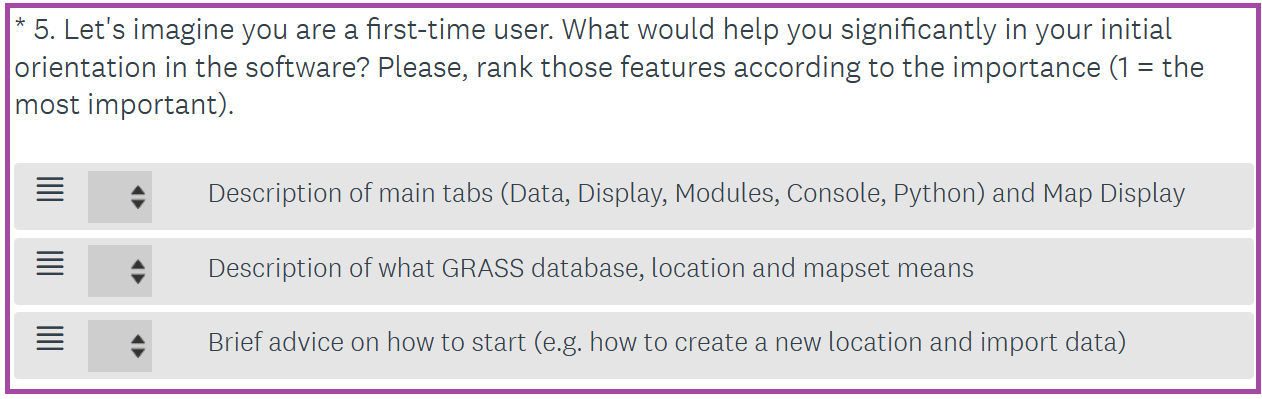
\includegraphics[width=16cm]{../pictures/ranking_question.png} 
\caption[A typical example of a Ranking question]{A typical example of a Ranking question (Source: Personal collection)}
\label{fig:ranking_question}
\end{center}
\end{figure}

\smallskip
\vspace*{-0.5cm}
\noindent \textbf {Comment Box}

\noindent This more sophisticated technique in terms of subsequent analyzes allows the user to share their own ideas in the form of open-ended responses. The basis of the analysis is to determine the topics into which the answers can be categorized. It may happen that one answer includes more topics.  In this case it is advantageous to divide the answers into atomic parts and then categorize them. Comment Box questions (see Fig. \ref{fig:comment_box_question}) can be further analyzed in a similar way as Multiple Choice types - by displaying the numbers of responses in individual topics using histograms.

\vspace{0.3cm}
\begin{figure}[hbt!] 
\begin{center}
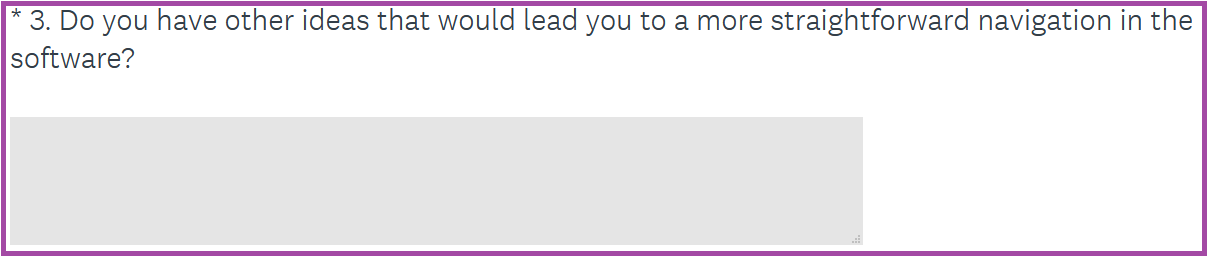
\includegraphics[width=15cm]{../pictures/comment_box_question.png} 
\caption[A typical example of a Comment Box question]{A typical example of a Comment Box question (Source: Personal collection)}
\label{fig:comment_box_question}
\end{center}
\end{figure}

\smallskip
\vspace*{-0.5cm}
\noindent \textbf {Multiple Choice}

\noindent For this type of question, we also distinguish whether the respondent can choose just one option or may check more than one. In this work, ``One option'' variant is used (see Figure \ref{fig:multiple_choice_question}). The disadvantage of the Multiple Choice question is the fact that we give the respondent a fixed list of answer option, which can skew the answers. Therefore, the ``Other (please specify)'' variant is usually added as a last place, which allows the user to write their own answer. The analysis of a question providing ``Other'' variant is more demanding and requires a similar approach as the Comment Box question since it has the character of an open-ended question. Therefore, the responses must first be organized into topics they deal with. If many people take the opportunity to write their own comment, it is likely that the responses for the question were not designed correctly. Then the assignment of open-ended responses to those originally set is more challenging and the telling value of responses is weakened.

\vspace{0.3cm}
\begin{figure}[hbt!] 
\begin{center}
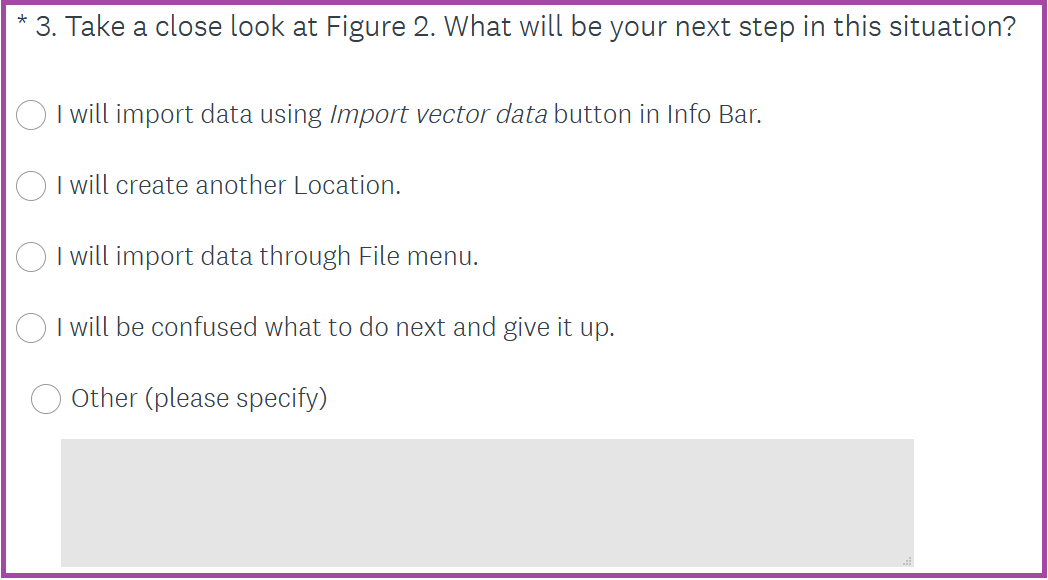
\includegraphics[width=14cm]{../pictures/multiple_choice_question.png} 
\caption[A typical example of a Multiple Choice question]{A typical example of a Multiple Choice question (Source: Personal collection)}
\label{fig:multiple_choice_question}
\end{center}
\end{figure}

\newpage
\vspace*{-1cm}
\fancyhead[RE, RO]{\fancyplain{}{\small \sl{Statistical methods of survey analysis}}}
\section{Statistical methods of survey analysis}
\label{sec:qstat}

\noindent In this work, a statistical analysis of questions is performed, which uses the basic methods of Explanatory Data Analysis. Thanks to this analysis, we can discover patterns or anomalies that occur in the answers. This can then help us to draw the conclusions of the surveys. It is important to understand EDA as a process that does not have given rules, it only depends on the analyst which of the methods to use. As this work is purely about finding out the basic features and characteristics of a relatively small sample of answers, which counts a maximum of 52 respondents (the number of respondents in the first part of the first survey), we analyze data over a single variable/column from a dataset. Therefore, we use only basic methods such as histograms, boxplots and probability density functions. Other EDA tools, for example, quantile-quantile (q-q) plots, scatter plots or correlation matrices detect relationships between two or more variables.

Ranking and Slider questions are analyzed using R language using RStudio. Here the author has applied extensive experience with this program, especially with the Tidyverse library, which is the core of data analysis in R and itself contains several interesting packages. In this work, the dplyr package is used for data manipulation. The vizualization is made through the ggplot2 \footnote{\url{https://github.com/rstudio/cheatsheets/blob/master/data-visualization-2.1.pdf}} package. In addition to the R language, the Python language has become the giant of data analysis with its Pandas library in recent years.

\subsection{Descriptive statistics}

Recently, descriptive statistics have also been included in EDA, which provides us with a brief summary of the data in the sense of Mean, Standard Deviation and 5 elements of the box whisker plot (Minimum, Maximum, 25th percentile, median and 75th percentile). The goal of descriptive statistics is to have a generalized view of data in order to prepare it for querying and vizualizing in different ways.

\smallskip
\noindent \textbf{Arithmetic mean}
\smallskip

\noindent This characteristic belongs to the measures of central tendency. It is simply the sum of all measurements divided by the number of observations in the data set. The mean is not a robust measure, it is highly sensitive to changes in data values. Therefore, it is the best measure for symmetric distributions without outliers. Other types of averages include weighted mean, geometric mean, harmonic mean.

\smallskip
\noindent \textbf{Median}
\smallskip

\noindent The median is the middle value that separates the higher half from the lower half of the data set. It is sometimes also called 2-quantile. In the case of a discrete random variable, the median is a number that satisfies the equality $ P(X \leq m) \geq 0.5$ and $P(X \geq m) \geq 0.5$ . In the case of a continuous real one-dimensional random variable with probability density $f$ the following applies to the median:
$$
\int_{-\infty}^{m} f(x)\, \mathrm{d}x = 0.5.
$$    

\noindent The median is a robust measure of central tendency. It means that is not very sensitive to changes in the data values. Therefore, it is useful for skewed distributions or data with outliers. Robust statistics in general are good for data drawn from a wide range of probability distributions, especially for distributions that are not normal.
 
 \smallskip
\noindent \textbf{Quartiles}
\smallskip

\noindent In general, a kth percentile of a data set is a value that divides the data set into the lower kth percentile and the upper (1 - kth) percentile. It means that k\% of the observations fall at or below kth percentile. The first quartile (Q1) is the 25th percentile and can be defined as the median value of the lower hall of data set. Similarly the third quantile (Q3) which is basically the75th percentile is the median of upper part of data set. The interquantile range (IQR) is defined as the difference between those quartiles.

\smallskip
\noindent \textbf{Standard deviation}
\smallskip

\noindent The standard deviation is simply the square root of the variance which indicates the average deviation of each data value from the mean of a data set. The calculation of the variance of a data set requires to compare each data value to the mean. The math formula for calculating the variance is simple:

$$
\sigma = \sqrt{\frac{\displaystyle\sum_{i=1}^{n}(x_i - \mu)^2} {n}}
$$

\noindent where n is the size of the sample and $\mu$ is the arithmetic mean.

The standard deviation provides the most commonly used measure of the spread of the underlying distribution of data. When comparing two distributions, the larger the standard deviation, the more dispersion the data set has (the data values differ more from the mean). 


\newpage
\vspace*{-1cm}
\subsection{Box-and-whisker plot}

\noindent This graphical method summarizes maximum and minimum values in data, the interquantile range and the median. It is very practical since all of those statistics can be seen at a glance. The graphical representation of individual parts of the graph is captured in Figure \ref{fig:boxplot}. The central box is enclosed by two lines corresponding to Q1 and Q3.  A line (or whisker) that extends from each edge of the box, goes to the farthest non-outlier point in the distribution. Outliers are points that fall more than 1.5 times the IQR from either edge of the box. Usually, they are plotted individually.

\vspace{0.3cm}
\begin{figure}[hbt!] 
\begin{center}
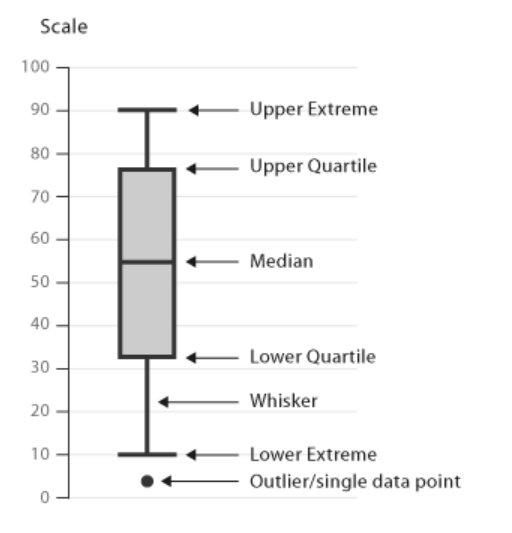
\includegraphics[width=7cm]{../pictures/boxplot.png} 
\caption[Description of box-and-whisker plot (boxplot)]{Description of box-and-whisker plot (boxplot) (Source: https://medium.com/code-heroku/introduction-to-exploratory-data-analysis-eda-c0257f888676)}
\label{fig:boxplot}
\end{center}
\end{figure}

\noindent We can identify symmetry or skewness of a distribution from a boxplot. And if more than one boxplot is plotted on the same scale, we can visually compare the centers, the spreads, and the extreme values of different variables.  Boxplots are very useful for both exploratory work and final presentation.

\subsection{Histogram vs. Bar Chart}

\noindent A histogram is used when working with quantitative data. It shows the number of observations that lie in-between the range of values, which is known as bin. Unlike a bar chart, individual columns touch. It indicates the underlying continuous nature of data. Categorical features cannot be visualized through histograms. Instead, we can use bar charts. In this type of graph, elements are taken as individual entities, so we can e.g. rearrange the blocks, from highest to lowest. To sum it up, histograms are used to show distributions of variables while bar charts are used to compare variables. An illustrative comparison of Histogram and Bar Chart is shown in the following Figure \ref{fig:histogram_barchart}:

\vspace{0.3cm}
\begin{figure}[hbt!] 
\begin{center}
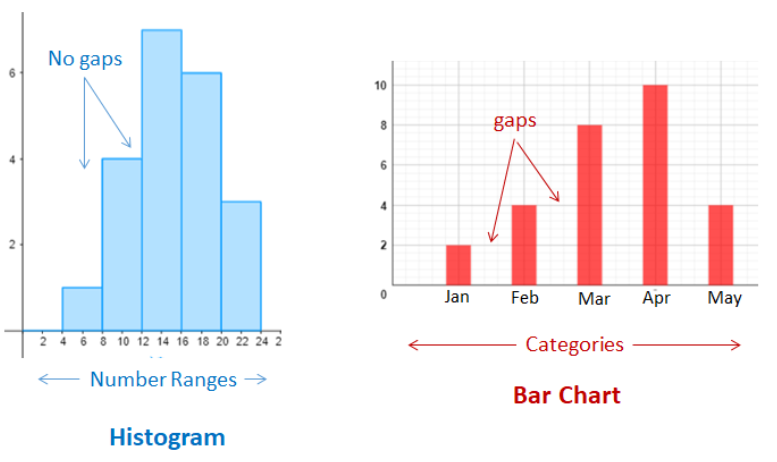
\includegraphics[width=12cm]{../pictures/histogram_barchart.png} 
\caption[Histogram vs. Bar Chart (boxplot)]{Histogram vs. Bar Chart (Source: https://www.onlinemathlearning.com/histograms.html)}
\label{fig:histogram_barchart}
\end{center}
\end{figure}

\subsection{Probability density function (PDF)}

Simply said the Probability density curve is the graphical representation of the probability that a contiouns random variable falls in a particular class. Therefore, the total area under an entire density curve is 100 \%. The probability that a continuous random variable acquires a certain (exactly given) value is zero. This follows from the following relation, from which it is possible to determine by an integral the probability that the random variable X acquires a value from the interval $ (x_1, x_2) $:

$$
P[x_1 \leq X \leq x_2] = \int_{x_1}^{x_2} f(x)\, \mathrm{d}x.
$$

\noindent For a discrete random variable, we determine the probability that it is equal to exactly some value. Such a function is called the Probability mass function (PMF). It holds that all probabilities in the function must be non-negative and together give the sum of 1. The value of the random variable having the largest probability mass is the mode.

\newpage
\vspace*{-1cm}
\subsection{Statistical methods used according to data types}

How to analyze survey responses depends on their type. We divide two types of variables - quantitative and quantitative. Qualitative (categorical) data cannot be quantified. Although numerical codes can be assigned to individual categories, they do not have a logical connection with quantity. Qualitative data can be further divided into binary (yes / no), nominal (contains more categories) and ordinal (also contains more categories and can be sorted). For example, very hot, hot, cold, very cold, warm are all nominal data when considered individually. But when placed on a scale and arranged in a given order (very hot, hot, warm, cold, very cold), they are regarded as ordinal data. Regarding descriptive statistics, we can count and determine a mode (the most common value in a dataset) for nominal data. Measures of central tendency for ordinal data, which values are ranked relative to each other but are not measured absolutely, are limited to mode or median. 

Examples of nominal qualitative data are the responses to questions of Multiple Choice type. Here, it is possible to create a bar chart (where we can find the mode), but other descriptive statistics do not make sense. An example of ordinal qualitative data are the responses to questions of Ranking type. A Bar Plot can also be compiled for Ranking questions, but the mean and standard deviation do not make sense. Ordinal variables are not continuous variables and should not be treated as if they are. Therefore, we should correctly create the Probability mass function (PMF) for Ranking questions where we determine a specific point probability on the y-axis that the discrete random variable is equal to some order. However, in the questions Q3 in the first part of the first survey and Q5 in the second part of the survey, PDF charts were eventually used. Although their use is not entirely correct, they provide better visual insight into the data than PMF, especially if we have several PDF charts for different variables.

Conversely, quantitative or numerical data can be characterized by a numerical value. Quantitative variables can be further classified as either discrete (those with a finite or countable number of possible values) or continuous (those with an infinite or un-countable number of possibilities). In the case of surveys conducted in this work, the Slider questions always have the same form - we measure the degree of agreement with the statement on a scale from 0 to 100. It is not a discrete variable, because we do not have any obvious categories from the beginning. Those classes have to be created. In this work, they were determined according to the SUS questionnaire: [0, 20] - Strongly disagree, (20, 40] - Disagree, (40, 60] - Neutral, (60, 80] - Agree and (80, 100] - Strongly agree.

%% -------<<< Chapter 4: Analysis of the results of the first survey>>>-------\\%%%%%%%%%%%%%%%%%%%%%%%%%%%%%%%%%%%%

\newpage
\vspace*{-1cm}
\fancyhead[RE, RO]{\fancyplain{}{\small \sl{Analysis of the results of the first survey}}}
\section{Analysis of the results of the first survey}
\label{sec:qstat}

\noindent The main part of this work consists of two questionnaires. The first questionnaire was released 23 October and stopped 29 October 2020. It has two separate parts. The first one contains six questions dealing with the improvement of the GRASS GIS startup mechanism and the assessment of the state after GSoC. The second part of the survey which is even more important for this master thesis contains 5 questions focusing on the enhancement of the newcomers' experience. In other words, it focuses on possibilities how to enrich existing Demolocation concept so that the new user can find his way around the software as quickly and conveniently as possible. The implementation part of this work is based on the second part of the first survey and then especially on the second survey, which was released roughly a month later and is analyzed in Section \ref{sec:2survey}.

\subsection{Part 1: GRASS startup and Data Catalog}

\noindent The first part of the survey returns to the changes that was implemented within the GSoC. It tries both - to get feedback from users and to answer questions that remain unanswered after GSoC. From this point of view, the most fundamental question is No. 2, which finds out the preferences regarding the way of starting GRASS GIS in a situation where the last mapset is not in a usable state. Questions 4, 5 and 6 are also related to the further direction of GRASS GIS (not only in terms of the startup mechanism) while questions 1 and 3 assess the benefits of GSoC. The first part of the survey was attended by 52 respondents, the completion rate was high - 96 \% and no respondent skipped any questions. We can see a weekly graph of the number of responses for a specific day in Fig. \ref{fig:survey1_part2_insight2}.

\begin{figure}[hbt!] 
\begin{center}
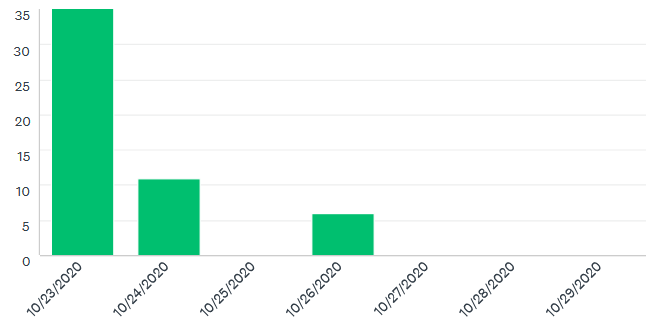
\includegraphics[width=10.5cm]{../surveys/analyzed_data/survey1_part1_insight2.png} 
\caption[Survey 1 Part 1: Responses by day]{Survey 1 Part 1: Responses by day (Source: Basic analyzes provided by the SM)}
\label{fig:survey1_part1_insight2}
\end{center}
\end{figure}

\newpage
\noindent \textbf{Question 1: What do you think about the following statement? \\
The partial removal of the startup screen and improvement of the Data Catalog simplifies the initial introduction to the software and further work.}
\par\noindent\rule{\textwidth}{0.4pt}
\noindent This question has the form of a Slider where 0 means complete disagreement with the statement and 100 means complete agreement. If we only worked with an average value of 70.9, we would conclude that enthusiasm probably prevails, but it is not so certain. The box-whisker-plot in Fig. \ref{fig:survey1_part1_question1_boxplot} shows that the median is significantly higher - 78.5 points out of a 100. If we look at the histogram in Figure \ref{fig:survey1_part1_question1_histogram}, which was divided into 5 parts exactly according to the number of bins in the original SUS, we can see that in the last interval ``Strongly agree'' there are 22 responses out of 52. On this basis we can conclude then that the vast majority like the situation after GSoC, however, there is also a minority of negative opinions.

\begin{figure}[hbt!] 
\begin{center}
\includegraphics[width=12cm]{../surveys/analyzed_data/survey1_part1_question1_excel_histogram.png} 
\caption[Survey 1 Part 1 Question 1: Histogram]{Survey 1 Part 1 Question 1: Histogram (Source: Personal collection)}
\label{fig:survey1_part1_question1_histogram}
\end{center}
\end{figure}

\vspace{0.3cm}
\begin{figure}[hbt!] 
\begin{center}
\includegraphics[width=10cm]{../surveys/analyzed_data/survey1_part1_question1_excel_boxplot.png} 
\caption[Survey 1 Part 1 Question 1: Boxplot]{Survey 1 Part 1 Question 1: Boxplot (Source: Personal collection)}
\label{fig:survey1_part1_question1_boxplot}
\end{center}
\end{figure}

\newpage
\noindent \textbf{Question 2: How do you think GRASS should start when the last mapset is not in a usable state (was deleted or is in use)?}
\par\noindent\rule{\textwidth}{0.4pt}
\noindent The result of this question put in the Multiple Choice form with the possibility of open-ended responses is very unexpected and unclear. Some open-ended answers strongly suggest that respondents did not understand from the previous context to the question (see Appendix \ref{appendix:A}, page 2) that the startup screen will not be visible at all in other cases. Another drawback is the only two close-ended choices. Most people therefore preferred something familiar (startup screen) to the new concept of Demolocation.

One of the ways to proceed here is not to give to the result of this question in terms of the bar chart in Figure \ref{fig:survey1_part1_question2_histogram_sm}, as the possibilities of answers to this question were not well conceived, and focus mainly on open-ended responses. Ten respondents choose neither of the two questions offered and took the opportunity to write their own proposal. Of the ten answers, which are categorized in the table in Fig. \ref{fig:survey1_part1_question2_other_answers}, only one respondent \#31 is for maintaining the original start screen. There are some ideas of displaying a simple dialog in the form of a warning message, which offers a user some other options - e.g. to open a demolocation, an existing mapset or to create own mapset. There was also a suggestion that it would not be a dialog, but only a pop-up message.

\vspace{0.3cm}
\begin{figure}[hbt!] 
\begin{center}
\includegraphics[width=17cm]{../surveys/analyzed_data/survey1_part1_question2_histogram_sm.png} 
\caption[Survey 1 Part 1 Question 2: Bar Chart]{Survey 1 Part 1 Question 2: Bar Chart (Source: Basic analyzes provided by the SM)}
\label{fig:survey1_part1_question2_histogram_sm}
\end{center}
\end{figure}

\vspace{0.3cm}
\begin{figure}[hbt!] 
\begin{center}
\includegraphics[width=15cm]{../surveys/analyzed_data/survey1_part1_question2_other_answers.pdf} 
\caption[Survey 1 Part 1 Question 2: Classification of open-ended responses]{Survey 1 Part 1 Question 2: Classification of open-ended responses (Source: Personal collection)}
\label{fig:survey1_part1_question2_other_answers}
\end{center}
\end{figure}

\noindent The first option, therefore, how this case could be solved would be to use the Info Bar, which would not have an informative character (as with the proposed solution for first-time users in second questionnaire), but would have the character of a warning. This Warning Info Bar explains why the user was redirected to Demolocation and instructs the user to open their own project.

The second solution is to create a simple startup screen, very similar to Moritz Lennert's Proposal B1\footnote{\url{https://trac.osgeo.org/grass/wiki/wxGUIDevelopment/New\_Startup\#Changeparadigm}}, which explains the situation to the user (the last mapset used has been deleted or is in use by another process) and suggests further steps.

The advantage of changes made after GSoC is that changing the database, location or mapset is very simple through the new Data Catalog, as well as saving and opening workspaces. Therefore, not only the author, but also other developers are inclined rather to the variant to completely remove any form of startup screen and employ Info Bars instead.

\par\noindent\rule{\textwidth}{0.4pt} \\
\noindent \textbf{Question 3: Please, rank how useful these features in Data Catalog would be (or already are) for you (1 = the most useful).}
\par\noindent\rule{\textwidth}{0.4pt}

\noindent This question asks the GRASS user to evaluate the benefits of the new features that were introduced after GSoC. The implementation of \textit{Small icons distinctive mapping, locations, GRASS databases, and layers (vector, raster)} is the work of Anna Petrasova, other functions are part of the implementations performed by the author. The evaluation of functions is performed by sorting them from the most useful (number 1) to the least useful (number 7).

According to the means in Figure \ref{fig:survey1_part1_question3_descriptive_stats_sm} the greatest success have \textit{New management icons for adding GRASS database, location, and mapset, and for downloading location}. However, the use of mean and standard deviation is quite misleading for ordinal types of variables. It is better to focus on the median whose values are in Figure \ref{fig:survey1_part1_question3_pdf} marked in a red box. The median is the smallest for \textit{Small icons distinquishing mapsets, locations, GRASS databases, and layers (vector, raster)}. Although the responses do not have the character of a continuous random variable and the Figure \ref{fig:survey1_part1_question3_pdf} is somewhat misleading in terms of statistics, \textit{Small icons distinquishing mapsets, locations, GRASS databases, and layers (vector, raster) } are also the most successful here. In second place there are \textit{New management icons for adding GRASS database, location, and mapset, and for downloading location} and in third place we can find \textit{Creating, renaming and deleting mapset or location}.

Interestingly, no special success was achieved by \textit{Adding multiple GRASS databases}, which were relatively difficult to implement. As can be seen from the stacked bar chart, the most controversial is \textit{Mapset access info (current, in use, and a different user)}, which some users rated as the most useful and a similar number of users as the least useful.

\vspace{0.3cm}
\begin{figure}[hbt!] 
\begin{center}
\includegraphics[width=16cm]{../surveys/analyzed_data/survey1_part1_question3_descriptive_stats_sm.png} 
\caption[Survey 1 Part 1 Question 3: Descriptive statistics]{Survey 1 Part 1 Question 3: Descriptive statistics (Source: Basic analyzes provided by the SM)}
\label{fig:survey1_part1_question3_descriptive_stats_sm}
\end{center}
\end{figure}

\vspace{0.3cm}
\begin{figure}[hbt!] 
\begin{center}
\includegraphics[width=16cm]{../surveys/analyzed_data/survey1_part1_question3_histogram.png} 
\caption[Survey 1 Part 1 Question 3: Stacked Bar Chart ]{Survey 1 Part 1 Question 3: Stacked Bar Chart (Source: Basic analyzes provided by the SM)}
\label{fig:survey1_part1_question3_histogram}
\end{center}
\end{figure}

\vspace{0.3cm}
\begin{figure}[hbt!] 
\begin{center}
\includegraphics[width=15.5cm]{../surveys/analyzed_data/survey1_part1_question3_boxplot_r.png} 
\caption[Survey 1 Part 1 Question 3: Boxplot]{Survey 1 Part 1 Question 3: Boxplot (Source: Personal collection - R analysis)}
\label{fig:survey1_part1_question3_boxplot_r}
\end{center}
\end{figure}

\vspace{0.3cm}
\begin{figure}[hbt!] 
\begin{center}
\includegraphics[width=15.5cm]{../surveys/analyzed_data/survey1_part1_question3_pdf.png} 
\caption[Survey 1 Part 1 Question 3: Probability Density Function]{Survey 1 Part 1 Question 3: Probability Density Function (Source: Personal collection - R analysis)}
\label{fig:survey1_part1_question3_pdf}
\end{center}
\end{figure}

\newpage
\noindent \textbf{Question 4: Which features would you like to add?}
\par\noindent\rule{\textwidth}{0.4pt}
\noindent From the point of view of the Data Catalog, there are, for example, proposals for the EPSG code shown after the location name, cloning the location, deleting multiple layers via the context menu, displaying space time datasets (STDS) or displaying saved workspaces. Regarding things unrelated to the Data Catalog, three users would like an easier and clearer way to add WMS/WFS using the new icon.

\begin{figure}[hbt!] 
\begin{center}
\includegraphics[width=16cm]{../surveys/analyzed_data/survey1_part1_question4_open_ended.png} 
\caption[Survey 1 Part 1 Question 4: Classification of open-ended answers]{Survey 1 Part 1 Question 4: Classification of open-ended answers (Source: Personal collection)}
\label{fig:survey1_part1_question4_open_ended}
\end{center}
\end{figure}

\newpage
\noindent \textbf{Question 5: Because we have limited screen space, we need to think about where we can add new features.Where would you add them?}
\par\noindent\rule{\textwidth}{0.4pt}
\noindent In this Multiple Choice question, most respondents agree to add additional functions to the context menu. Interestingly, 13.5 \% of respondents think that no additional features should be added, that there is little space for them. That is almost a seventh of the respondents, so also a relatively significant part. So there is a certain fear that the added functions will not rather detract from the clarity of the current solution. Related to this is the fact that in the previous question number 4 none of respondents mention adding more complex functions to Data Catalog, such as Import Data. The improvements mainly concern the management of data hierarchy in GRASS.

\vspace{0.3cm}
\begin{figure}[hbt!] 
\begin{center}
\includegraphics[width=17cm]{../surveys/analyzed_data/survey1_part1_question5_descriptive_stats_sm.png} 
\caption[Survey 1 Part 1 Question 5: Bar Chart]{Survey 1 Part 1 Question 5: Bar Chart (Source: Basic analyzes provided by the SM)}
\label{fig:survey1_part1_question5_descriptive_stats_sm}
\end{center}
\end{figure}

\newpage
\noindent \textbf{Question 6: So, what do you think about the following statement? I would start GRASS using the file association of the workspace file (.gxw) frequently.}
\par\noindent\rule{\textwidth}{0.4pt}
\noindent This question takes the form of a Slider and was intentionally conceived in this somewhat strict way. It depends on the opinion of individuals whether they would really use this functionality often, not on the general belief, which can be distorted by the fact that in other software this functionality is a matter of course. GRASS GIS is the only software of those selected in the section \ref{sec:startup_concepts}, together with ILWIS, that does not have this option (see the summary \ref{subsec:startup_concepts_summary}). Nevertheless, based on the results of this question, GRASS GIS users do not seem to mind. The author can name several reasons why this is the case.

After changes within GSoC GRASS GIS starts in the last open mapset to the Data tabs, which allows easy switching between mapsets, opening other GRASS databases, saving and opening workspaces, etc. It is therefore very easy to work with data hierarchy in GRASS GIS. In addition, the data is stored directly in the mapsets, so it is not necessary to remember where in the disk the data is located, such as in QGIS. Another reason is that GRASS GIS is often used under the Unix operating system and runs from the command line.

The answer to this question is therefore very ambiguous about what to expect. The average value of the degree of agreement with the statement is 51, as you can see from Fig. \ref{fig:survey1_part1_question6_boxplot}. The median is slightly higher, just over 54 points. Both of these values are more or less meaningless. The most interesting view is offered by the Probability Density Function in Fig. \ref{fig:survey1_part1_question6_r_pdf}. The largest density values are in the range of 50 - 75, according to which we can conclude that the answer whether to implement is rather yes, but it is not a functionality that is perceived by GRASS GIS users as essential.

\vspace{0.3cm}
\begin{figure}[hbt!] 
\begin{center}
\includegraphics[width=13cm]{../surveys/analyzed_data/survey1_part1_question6_boxplot.png} 
\caption[Survey 1 Part 1 Question 6: Boxplot]{Survey 1 Part 1 Question 6: Boxplot (Source: Personal collection)}
\label{fig:survey1_part1_question6_boxplot}
\end{center}
\end{figure}

\vspace{0.3cm}
\begin{figure}[hbt!] 
\begin{center}
\includegraphics[width=14cm]{../surveys/analyzed_data/survey1_part1_question6_histogram.png} 
\caption[Survey 1 Part 1 Question 6: Histogram]{Survey 1 Part 1 Question 6: Histogram (Source: Personal collection)}
\label{fig:survey1_part1_question6_histogram}
\end{center}
\end{figure}

\vspace{0.3cm}
\begin{figure}[hbt!] 
\begin{center}
\includegraphics[width=15cm]{../surveys/analyzed_data/survey1_part1_question6_r_pdf.png} 
\caption[Survey 1 Part 1 Question 6: Probability Density Function]{Survey 1 Part 1 Question 6: Probability Density Function (Source: Personal collection - R analysis)}
\label{fig:survey1_part1_question6_r_pdf}
\end{center}
\end{figure}


\newpage
\vspace*{-1cm}
\subsection{Part 2: Better first-time user experience in GRASS}

\noindent The second part of the survey seeks to get user preferences on how they would like to improve the first-time user experience. This survey consists mainly of Multiple Choice and Comment Box types of questions, so the evaluation is very subjective and there are exceptional answers for which the author was not entirely sure whether she understood them correctly. This is, after all, one of the disadvantages of questionnaires and remote usability testing in general.

This part of the survey offers two ways to improve the first-time user experience that the author has noticed with other software - Info Bars (QGIS 3) and First Run Wizard (Zoner Photo Studio X). Respondents evaluate these topics in the first two questions, thus giving feedback which of the above options they would prefer in GRASS. Question number 3 is very open and users write their own suggestions on how to improve the first-time user experience. In question 4, users share ideas for software that is user-friendly. In question 5, we then find out which specific things cause problems for users and what any first-time advice should be about. The second part of the first survey was attended by 46 respondents, the completion rate was high - 97 \%. Question 4, which was optional, was skipped 14 times. Other questions were answered by all participants, however, the answers were not always relevant, so not all are part of the analyzes. We can see a weekly graph of the number of responses for a specific day in Fig. \ref{fig:survey1_part2_insight2}.

\vspace{0.3cm}
\begin{figure}[hbt!] 
\begin{center}
\includegraphics[width=15cm]{../surveys/analyzed_data/survey1_part2_insight2.png} 
\caption[Survey 1 Part 2: Responses by day]{Survey 1 Part 2: Responses by day (Source: Basic analyzes provided by the SM)}
\label{fig:survey1_part2_insight2}
\end{center}
\end{figure}

\newpage
\noindent \textbf{Question 1: Do you like the idea of First Run Wizard (inspired by Zoner implementation)?}
\par\noindent\rule{\textwidth}{0.4pt}
\noindent Users mostly like the idea of First Run Wizard, but there are also a lot of comments in Figure \ref{fig:survey1_part2_question1_all} highlighted in pink, which First Run Wizard finds rather annoying. After all, comments 1 and 2 also mean ``No, because...'' rather than ``Yes, but...''. If we then combine the subgroups into two large groups ``Yes'' and ``No'', we will come to the conclusion that 33 (71.7 \%) respondents are for and the remaining 13 (28.3 \%) respondents against First Run Wizard.

\vspace{0.3cm}
\begin{figure}[hbt!] 
\begin{center}
\includegraphics[width=15cm]{../surveys/analyzed_data/survey1_part2_question1_all.png} 
\caption[Survey 1 Part 2 Question 1: Bar Chart, descriptive statistics and open-ended responses]{Survey 1 Part 2 Question 1: Bar Chart, descriptive statistics and open-ended responses (Source: Basic analyzes provided by the SM)}
\label{fig:survey1_part2_question1_all}
\end{center}
\end{figure}

\noindent The comment \#2 recommends creating pop-ups that themselves contain only the most important information, but refer to a written and video tutorial. So, the point is to include as few distractions as possible in the software itself, but to refer well to detailed information, for example in the form of a ``Learn more'' button.

\par\noindent\rule{\textwidth}{0.4pt}
\noindent \textbf{Question 2: Do you like the idea of first-time mode info bars (visually similar to info bars in QGIS implementation)?}
\par\noindent\rule{\textwidth}{0.4pt}

\noindent People largely like both the Info Bars and the First Run Wizard. However, there are fewer ``Yes, but...'' comments in Info Bars, and unlike the previous question, they are literally ``Yes, but...'', as we can see in Figure \ref{fig:survey1_part2_question2_all}. 

\vspace{0.3cm}
\begin{figure}[hbt!] 
\begin{center}
\includegraphics[width=15.5cm]{../surveys/analyzed_data/survey1_part2_question2_all.png} 
\caption[Survey 1 Part 2 Question 2: Bar Char descriptive statistics and classification of open-ended responses]{Survey 1 Part 2 Question 2: Bar Char, descriptive statistics and classification of  open-ended responses (Source: Basic analyzes provided by the SM)}
\label{fig:survey1_part2_question2_all}
\end{center}
\end{figure}

\noindent A relatively large proportion of respondents (17.4 \%) think that these icons will be ignored by new GRASS users. If we combine the subgroups into two main groups ``Yes'' and ``No'', we conclude that 34 (73.9 \%) respondents are for and 12 (26.1 \%) against Info Bars. This is a slightly better balance than in question number 1. But even here we must be careful. The difficult task will be to find a compromise between the fact that the information icons must be placed in the right place so that the user can ignore them as little as possible, but at the same time must not act as a warning, which is also pointed out by comment \#3.

\par\noindent\rule{\textwidth}{0.4pt}
\noindent \textbf{Question 3: Do you have other ideas that would lead you to a more straightforward navigation in the software?}
\par\noindent\rule{\textwidth}{0.4pt}
\noindent For this question, GRASS GIS users were very shared, which resulted in a very detailed analysis of the answers into 12 groups. However, the variety of responses is so wide that many responses could not be included, so they ended up in a separate ``Other'' group. In the following lines, the author summarize and discuss in more detail several opinions that were expressed. In the survey, several opinions are expressed, which the author will try to summarize and discuss in more detail in the following lines. The color represented by the categories in Figures \ref{fig:survey1_part2_question3_open_ended-1_1}, \ref{fig:survey1_part2_question3_open_ended-2_1}, \ref{fig:survey1_part2_question3_open_ended3_1} is purely random.

The first topic that permeates basically the whole questionnaire is how to better explain the GRASS GIS data hierarchy to newcomers. In this question, this topic is mentioned by respondents \#2, \#8, \#19, \#22. For example, respondent \#8 suggests a ``First Time Help'' pop-up window that explains to a user folders on disk, location, etc. However, the topic of GRASS data hierarchy appears in other questions as well. For example, in question 4 respondent \#1 talks about the old concept of location. However, as can be seen from the answers \#25 and \#27, there are also users who are satisfied with the current system.

Either way, data hiearchy in GRASS is usually one of the main topics of video calls of the developer community (link to the attached video call) and the only agreement is that the concept of database/location/mapset is abstruse to new users. The truth is that if database/location/mapset were named differently and more intuitively (for instance database/project/subproject) and thus closer to the standard of other open-source software, then the word ``old'' would not be part of the criticism. Therefore, perhaps the most feasible proposal that will not interfere so much with the implementation of GRASS is to maintain the concept, but to change the terminology.

The second important topic is better documentation, for example with the use of videos. Respondent \#26 would even like a very detailed PDF manuals with printscreens and information on each button and functionality.

\newpage
\vspace{0.3cm}
\begin{figure}[hbt!] 
\begin{center}
\includegraphics[width=17cm]{../surveys/analyzed_data/survey1_part2_question3_open_ended-2_2.png} 
\caption[Survey 1 Part 2 Question 3: Classification of open-ended responses - part 1]{Survey 1 Part 2 Question 3: Classification of open-ended responses - part 1 (Source: Personal collection)}
\label{fig:survey1_part2_question3_open_ended-1_1}
\end{center}
\end{figure}

\newpage
\vspace{0.3cm}
\begin{figure}[hbt!] 
\begin{center}
\includegraphics[width=16cm]{../surveys/analyzed_data/survey1_part2_question3_open_ended-2_3} 
\caption[Survey 1 Part 2 Question 3: Classification of open-ended responses - part 2]{Survey 1 Part 2 Question 3: Classification of open-ended responses - part 2 (Source: Personal collection)}
\label{fig:survey1_part2_question3_open_ended-2_1}
\end{center}
\end{figure}

\newpage
\vspace{0.3cm}
\begin{figure}[hbt!] 
\begin{center}
\includegraphics[width=15cm]{../surveys/analyzed_data/survey1_part2_question3_open_ended-2_1} 
\caption[Survey 1 Part 2 Question 3: Classification of open-ended responses - part 3]{Survey 1 Part 2 Question 3: Classification of open-ended responses - part 3 (Source: Personal collection)}
\label{fig:survey1_part2_question3_open_ended3_1}
\end{center}
\end{figure}

\noindent  It should be noted here that the proposed solutions that will improve the first-time user experience must be sustainable also in terms of further development, which will probably be crucial in the future, as the community around GRASS is very lively. Therefore, it is definitely advantageous to focus on smaller outputs, which is easy to edit in case of changes, rather than doing ``inflexible'' tutorials, whether in the form of PDFs or videos, which can be very outdated in a short time, thus for new users rather confusing. However, this does not mean that short videos or clearer documentation could not be created. Inspiration can come here from QGIS, as suggested by respondent \#14 in question 5. The respondent \#7 also encounters the relationship between QGIS and GRASS. As mentioned in \ref{subsection:GIS software} GRASS modules can also be run through QGIS. However, the GRASS function in QGIS has a different description than the same module in GRASS. This should definitely be unified on the GRASS side.
 
From the point of view of the further direction of this master thesis, a very important topic is how to improve the first-time user experience directly in the software, in other words how to improve demolocation where GRASS starts automatically after the first start. The answer \#3 is closely related to this since it asks for immediate display of the map. It definitely makes sense. After all, for example, the open-source software Blender for modeling and rendering 3D computer graphics shows the cube when started. It is therefore natural for a new GRASS user to see the map. Furthermore, the classification also shows that brief advice on how to start would be valuable for newcomers and six respondents (\#5, \#8, \#9, \#12, \#15, \#18) mentions some form of info icons. Respondents \#5 and \#12 also point out the importance of the initial data and its easy import into GRASS GIS. There are also two opinions which call for putting GRASS into a single window.

The answers also point out some of the problems that users face without explicitly mentioning them. Respondents \#10 and \#11 want Tool search which is already part of the Modules tab. This may indicate that users did not understand the meaning of other tabs (probably did not notice them). By the way, the Question 5 also draws attention to this problem, where 9 respondents out of 46 classified \textit{Description of main tabs (Data, Display, Modules, Console, Python] and Map Display} as the advice that would help them most in their initial orientation in the software.

\par\noindent\rule{\textwidth}{0.4pt}
\noindent \textbf{Question 4: What software do you think does a good job of providing a good first-time user experience? (optional)}
\par\noindent\rule{\textwidth}{0.4pt}
\noindent In this open optional question, QGIS is mentioned most often. However, the solution in GRASS may not be the same as in QGIS. Ideally it will be the best solution for GRASS, see \#42 in Q3.

\vspace{0.3cm}
\begin{figure}[hbt!] 
\begin{center}
\includegraphics[width=16cm]{../surveys/analyzed_data/survey1_part2_question4_open_ended_1.png} 
\caption[Survey 1 Part 2 Question 4: Classification of open-ended responses]{Survey 1 Part 2 Question 4: Classification of open-ended responses (Source: Personal collection)}
\label{fig:survey1_part2_question4_open_ended_1}
\end{center}
\end{figure}

\newpage
\noindent \textbf{Question 5: Let's imagine you are a first-time user. What would help you significantly in your initial orientation in the software? Please, rank those features according to the importance (1 = the most important).}
\par\noindent\rule{\textwidth}{0.4pt}
\noindent This question, where users sorted different features according to how much they would help them in their initial orientation, has no clear answers at all. Although the \textit{Description of main tabs (Data, Display, Modules, Console, Python] and Map Display} variant has the highest median (see Fig. \ref{fig:survey1_part2_question5_stats}) it appears very often on the first place as captured by the bar chart in Figure \ref{fig:survey1_part2_question5_histogram_r}. The answers suggest that the software should provide advice on all of these selected aspects, because more or less, all of these aspects are problematic for new users. The question remains what advice and in what form to include directly in the demolocation and what advice should no longer be included, but it should be well referred to.
    
\vspace{0.3cm}
\begin{figure}[hbt!] 
\begin{center}
\includegraphics[width=16cm]{../surveys/analyzed_data/survey1_part2_question5_stats.png} 
\caption[Survey1 Part 2 Question 5: Descriptive statistics]{Survey1 Part 2 Question 5: Descriptive statistics (Source: Personal collection - R analysis)}
\label{fig:survey1_part2_question5_stats}
\end{center}
\end{figure}

\vspace{0.3cm}
\begin{figure}[hbt!] 
\begin{center}
\includegraphics[width=15cm]{../surveys/analyzed_data/survey1_part2_question5_histogram_r.png} 
\caption[Survey1 Part 2 Question 5: Stacked Bar Chart]{Survey1 Part 2 Question 5: Stacked Bar Chart (Source: Personal collection - R analysis)}
\label{fig:survey1_part2_question5_histogram_r}
\end{center}
\end{figure}

\newpage
\vspace*{-1cm}
\fancyhead[RE, RO]{\fancyplain{}{\small \sl{GRASS GIS Development Proposals}}}
\section{GRASS GIS Development Proposals}
\label{sec:proposal}

\newpage
\vspace*{-1cm}
\fancyhead[RE, RO]{\fancyplain{}{\small \sl{How to enhance first-time user experience}}}
\subsection{How to enhance first-time user experience: Proposal}
\label{sec:proposal1}


Jak bylo popsáno v úvodu a v podkapitole Suggestions, tato práce se skládá ze 2 na první pohled nezávislých částí. První část (hlavní část této práce) související s druhou části prvního průzkumu a s druhým průzkumem vylepšuje koncept defaultní lokace o tzv. first-time user mode, který má za úkol vylepšit first-time user experience.  Druhá část související s první částí prvního průzkumu výrazně navazuje na změny provedené v rámci GSoC a odstraňuje nedostatky nového startovacího mechanismu, které v rámci GSoC nebyly zcela dořešeny. První hlavní téma této práce se soustředí výhradně na nové uživatele, zatímco druhé téma související s úplným odstraněním původní startovací obrazovky (aby se neobjevovala ani i v situaci kdy last mapset is not in usable state) je tématem, které se dotkne všech stávajících uživatelů.



\vspace{0.3cm}
\begin{figure}[hbt!] 
\begin{center}
\includegraphics[width=16cm]{../pictures/first-time_user_diagram.pdf} 
\caption[Info Bars Flowchart for first-time user]{Info Bar Flowchart for first-time user (Source: Personal collection)}
\label{fig:first-time_user_diagram}
\end{center}
\end{figure}

\newpage
\vspace*{-1cm}
\fancyhead[RE, RO]{\fancyplain{}{\small \sl{How to create better GRASS GIS startup}}}
\subsection{How to create better GRASS GIS startup}
\label{sec:proposal1}

In the first part of the first survey, Q4 and Q5 mainly concern the Data Catalog and Management Icons, which is definitely important for future software development, however, the implementation is beyond the scope of this work. From the point of view of this work, the most important question is number 2, which solves the case when GRASS wants to start in the last used mapset, however, this mapset is not available for one of these reasons - it has either been deleted or it is used by another process. Unfortunately, this question was not drafted very cleverly in terms of the answer options offered, which is evident from the large number of open-ended responses.

At first glance, the number of respondents who would choose the modernized version of startup screen prevails. However, only 2 out of 10 open-ended responses suggest some form of startup screen. Although the total number of respondents proposing a startup screen is 34 (32 + 2), ie. 65 \% percent of all respondents, we can not talk about a significantly majority opinion. In addition, in open-ended responses, ideas with some form of information or error message very often appear, which is a very interesting variant, which the author of the work did not think of when compiling the survey. In terms of implementation complexity, however, it is a simple option, as the proposed Info Bar for first-time users can cover both purposes - it will primarily serve as a help for new users and secondarily it can serve as an information channel for existing users. In the latter context, they can inform them about non-standard situations and speed up user's work (e.g. when creating a location, it will automatically offer the creation of a mapset, etc.). The Flowchart simulating the startup mechanism of an existing GRASS GIS user is shown in Figure \ref{fig:normal_user_diagram}.

 As we can see, if the last used mapset cannot be used, we come across two different situations:

\noindent \textbf{Either the last used location (as the parent of the last used mapset) is on the disk or it is not.} 

\begin{itemize}
\item If the last used location is not found, it means only one thing, the user deleted the location, so it is not possible to find the last used mapset. In this case, there is nothing to choose from but start GRASS to the default location.
\item If the last used location is found and at the same time the PERMANENT mapset is not used by another process in this location, GRASS can start in this PERMANENT mapset.
\end{itemize}

The default location is therefore taken as the last unwelcome option employed only when the last used location either does not exist at all or exists, but it is not possible to open the last used mapset or PERMANENT mapset. In both cases, the user will see the notification in the form of a warning Info Bar saying the reason of start in default location and advicing a user on what to do next in this situation. The solution is simple as in the new version of the Data Catalog after GSoC it is very easy to add a new database to the Data Catalog, create a new location, etc. 

Since these messages are closely related to the Data Catalog and data hierarchy in GRASS GIS in general, we can use exactly the same object of Info Bar which is used for messages intended for first-time users. This Info Bar is created each time the user starts GRASS GIS and it will only be up to the situation what message will be displayed. During the work, the user can then close the Info Bar, however, in reality it is only hidden and in another defined situation, it  may appear again.

\vspace{0.3cm}
\begin{figure}[hbt!] 
\begin{center}
\includegraphics[width=17cm]{../pictures/normal_user_diagram.png} 
\caption[Info Bars Flowchart for any existing user]{Info Bar Flowchart for any existing user (Source: Personal collection)}
\label{fig:normal_user_diagram}
\end{center}
\end{figure}

We could also think of other situations where the Info Bar could be displayed to users. For example, when creating a new location, it can be assumed that the user will subsequently request the creation of a mapset. Similarly, when creating a database, it can be assumed that the user will want to create a new location in the next step. The notifications could therefore be a kind of guide not only for the initial user, but also for more experienced users. Their purpose would be to speed up the user's work related to organization of their data.

%% -------<<< Chapter 6: Analysis of the results of the second survey>>>-------\\%%%%%%%%%%%%%%%%%%%%%%%%%%%%%%%%%%%%

\newpage
\vspace*{-1cm}
\fancyhead[RE, RO]{\fancyplain{}{\small \sl{Analysis of the results of the second survey}}}
\section{Analysis of the results of the second survey}
\label{sec:qstat2}

\noindent The second questionnaire was released on November 26 and stopped on November 30, 2020. It introduces a new Info Bars solution to new and existing users and tests its success. At the same time, it addresses users to share their own ideas on how to modify and adapt the solution so that the resulting solution that emerges from this work, largely based on this survey, enriches the first-time user experience with GRASS as much as possible.

The questionnaire is based on a simple task. A user has vector data of rivers in the Czech Republic in the shapefile format in the coordinate system S-JTSK/Krovak East North (EPSG:5514) and they would like to import this data into GRASS and perform a simple task - extract a river called Otava and save it in a separate layer. Unfortunately, due to external epidemiological circumstances, this task could not be tested among GRASS beginners directly on the software. Thus, a survey was designed that simulates three key situations that, according to the diagrams in the previous chapter, a new user is likely to get into and which, according to the results of the second part of the first survey, are crucial. In these situations, the respondent is presented with software mockups of Info Bars which (if they are placed in the right place at the right time and correctly designed in terms of text) should lead to the right decision on how to continue in work. In the following text, the term \textit{default location} is preferred to the term \textit{demolocation}, which is more of a technical (developer) nature. Semantically, these concepts do not differ.

\textbf{The first situation} shown in the mockup in Fig. \ref{fig:grass_infobar_1} shows the GRASS GIS immediately after startup. At this point, a user needs find their way around in a completely unknown environment as quickly as possible and import their data so that he can look at it and possibly perform analyzes. The software starts in the Data tab to the default location (so-called demolocation), which in the Map Display window displays the world map in the WGS 84 system (EPSG:4326). The task of demolocation is to give the user a certain sense of security by showing a map and at the same time an example of data organization in the Data Catalog, which is now the center of GRASS. At the first moment, it is therefore essential for the user to at least passively understand the principle of the GRASS data hierarchy, which is well visible in the Data Catalog and is also briefly explained in the first Info Bar. In order to properly figure out the first situation, a user must realize that the data he wants to import into the software has a different coordinate system (EPSG:5514) than the one defined for the default location (EPSG:4326). This means that if a user understands the meaning of the location, he will create a new location that will have the coordinate system of the data he wants to import.

\vspace{0.3cm}
\begin{figure}[hbt!] 
\begin{center}
\includegraphics[width=17cm]{../pictures/grass_infobar_1.png} 
\caption[Survey 2: Situation 1]{Survey 2: Situation 1 (Source: Personal collection)}
\label{fig:grass_infobar_1}
\end{center}
\end{figure}

\newpage
\noindent Once a user creates a new location, he finds themselves in \textbf{the second situation} captured in Figure \ref{fig:grass_infobar_2} which displays the second Info Bar leading to data import. This Info Bar also explains the concept of PERMANENT mapset and shows a variant of creating own mapset, which is not necessary but useful. This means that we are still partially dealing with the topic of data hierarchy in GRASS, but at the same time we advise the user on how to import their data. After successful import, a map is automatically displayed in the Map Display.

\vspace{0.3cm}
\begin{figure}[hbt!] 
\begin{center}
\includegraphics[width=17cm]{../pictures/grass_infobar_2.png} 
\caption[Survey 2: Situation 2]{Survey 2: Situation 2 (Source: Personal collection)}
\label{fig:grass_infobar_2}
\end{center}
\end{figure}

\noindent The result of Question 5 of the second part of the first survey shows that users also have a problem with the meaning of individual tabs. After importing the data, a user wants to either analyze data directly or change its display in the Map Display (e.g. change transparency, strength, line color, etc.). In \textbf{the third situation} shown in Fig. \ref{fig:grass_infobar_3} it is therefore necessary to introduce a user to the two main tabs called Modules and Display, which he will need for mentioned purposes. As a reader probably noticed, the proposal seeks to provide new users with basic advice on all of the aspects that appeared in the Survey 1 Part 2 Question 5.

\vspace{0.3cm}
\begin{figure}[hbt!] 
\begin{center}
\includegraphics[width=17cm]{../pictures/grass_infobar_3.png} 
\caption[Survey 2: Situation 3]{Survey 2: Situation 3 (Source: Personal collection)}
\label{fig:grass_infobar_3}
\end{center}
\end{figure}

\noindent The survey was visited by 32 respondents and 25 of them provided relevant responses. The completion rate among relevant respondents was 96 \%. We can see a weekly graph  of the number of responses for a specific day in Fig. \ref{fig:survey1_part2_insight2}.

\vspace{0.3cm}
\begin{figure}[hbt!] 
\begin{center}
\includegraphics[width=10cm]{../surveys/analyzed_data/survey2_insight2.png} 
\caption[Survey 2: Responses by day]{Survey 2: Responses by day (Source: Basic analyzes provided by the SM)}
\label{fig:survey2_insight2}
\end{center}
\end{figure}

\noindent The questionnaire consists of a 10 questions - 6 questions concern the understanding of individual situations, 2 questions are complementary and two more questions find out how experienced the interviewer is - both in terms of GIS in general and in terms of GRASS GIS. 

The responses were divided into two groups with regard to the GRASS experience of individual respondents. The first group called \textbf{Occasional GRASS users} includes respondents who use GRASS less than sometimes (they chose less than 50 points in Q10) while the second group called \textbf{Frequent GRASS users} includes users who use GRASS more often than sometimes (they selected more than 50 points or 50 points in Q10). 

According to Q9, the \textbf{Occasional GRASS users} group (see Fig. \ref{fig:survey2_respondents_group1}) consists mainly of beginners and a minority of advanced or intermediate GIS experts (a total of 10 respondents) while the \textbf{Frequent GRASS users} group (see Fig. \ref{fig:survey2_respondents_group2}) includes mainly GIS professionals and some intermediate (a total of 15 respondents).

\vspace{0.3cm}
\begin{figure}[hbt!] 
\begin{center}
\includegraphics[width=11.5cm]{../surveys/analyzed_data/survey2_respondents_group1.png} 
\caption[Survey 2: GIS proficiency of \textbf{Occasional GRASS users} group]{Survey 2: GIS proficiency of \textbf{Occasional GRASS users} group (Source: Personal collection)}
\label{fig:survey2_respondents_group1}
\end{center}
\end{figure}

\begin{figure}[hbt!] 
\begin{center}
\includegraphics[width=11.5cm]{../surveys/analyzed_data/survey2_respondents_group2.png} 
\caption[Survey 2: GIS proficiency of \textbf{Frequent GRASS users} group]{Survey 2: GIS proficiency of \textbf{Frequent GRASS users} group (Source: Personal collection)}
\label{fig:survey2_respondents_group2}
\end{center}
\end{figure}

\newpage
\noindent Questions Q2, Q4, Q6, and Q8 has a type of Comment Box, which means that respondents shared their feelings and ideas in the form of open-ended responses. These are divided into six categories throughout the Survey 2:

\begin{enumerate}
\item Demolocation/Info Bar confused
\item Info Bar could be ignored
\item Terminology should be changed
\item Info Bar too long / Editing of content in Info Bar
\item Info Bar Helped
\item Other
\end{enumerate}

\noindent The answers in Figures \ref{fig:survey2_question2}, \ref{fig:survey2_question4}, \ref{fig:survey2_question6} and \ref{fig:survey2_question8} are sorted from the most serious category to the least serious. Only the last sixth category varying in importance and consists of responses that do not fall into any of the previous categories. The following lines analyze in detail the answers from Q1 - Q8 with regard to the user experience that arises from Q9 and Q10.

\par\noindent\rule{\textwidth}{0.4pt}
\noindent \textbf{Question 1: What will be your next step in first situation?}
\par\noindent\rule{\textwidth}{0.4pt}

\noindent There was only one correct choice for this Multiple Choice answer, namely ``I will create a new Location ''. The first situation was solved correctly by 17 out of 25 respondents (see Figures \ref{fig:survey2_question1_histogram_group1}, \ref{fig:survey2_question1_histogram_group2}). In the \textbf{Occasional GRASS users} group, 5 respondents solved it correctly, i.e., half of them. Even though the sample of users is very small, half of the people is definitely a success, because without help, a very new or little experienced user probably wouldn't have thought to create a new location at all.

\par\noindent\rule{\textwidth}{0.4pt}
\noindent \textbf{Question 2: Is something confusing to you? If so, what specifically?? (Optional)}
\par\noindent\rule{\textwidth}{0.4pt}

\noindent This open-ended optional question was answered by 9 respondents and comments can be seen in Figure \ref{fig:survey2_question2}. As the respondent \#21 points out, it is somewhat confusing that the default location contains two mapsets - not only the PERMANENT mapset, which must be included in each location, but also the user-named mapset. The world map is intentionally placed in the PERMANENT mapset, because this mapset is intended for storing and displaying basic data. However, analyzes should always be performed in a mapset other than PERMANENT. Therefore, at the end of GSoC, it was decided that the default location will also contain a user-named mapset set as \textbf{current},  which will motivate users not to use PERMANENT mapset for their further analyzes, but to sort their data into other mapsets. However, from the point of view of GRASS, this solution does not make sense, because in all other cases but default location we are only allowed to display layers from the current mapset, and when displaying layers from another mapset we need switch to it. Due to these circumstances, it would be probably more correct and at the same time more clearer for first-time users if the demolocation contained only the PERMANENT mapset with the included world map. After all, advice on the use of other mapsets is already part of the Info Bar in the second situation. Alternatively, a brief explanation of the term mapset could still be part of the first Info Bar, as suggested by the respondent \#24.

The response \#11 indicates that a user may not realize that he or she is in a default location at all. This would definitely need to be emphasized more. Respondents \#13 and \#17 fear that users will ignore the Info Bar. So another important step would be to think about how to highlight the Info Bar as much as possible so that most new users can really read it. However, as we can see from the responses \#10 and \#24 as well as from the number of correct answers in Q1, the Info Bar, even in the form in which it appears in this initial proposal, is certainly an improvement for new GRASS GIS users.

\vspace{0.3cm}
\begin{figure}[hbt!] 
\begin{center}
\includegraphics[width=14cm]{../surveys/analyzed_data/survey2_question1_histogram_group1.png} 
\caption[\textbf{Occasional GRASS users}: Bar Chart  for Question 1 from Survey 2]{\textbf{Occasional GRASS users}: Bar Chart for Question 1 from Survey 2 (Source: Personal collection)}
\label{fig:survey2_question1_histogram_group1}
\end{center}
\end{figure}

\vspace{0.3cm}
\begin{figure}[hbt!] 
\begin{center}
\includegraphics[width=13.5cm]{../surveys/analyzed_data/survey2_question1_histogram_group2.png} 
\caption[\textbf{Frequent GRASS users}: Bar Chart for Question 1 from Survey 2]{\textbf{Frequent GRASS users}: Bar Chart for Question 1 from Survey 2 (Source: Personal collection)}
\label{fig:survey2_question1_histogram_group2}
\end{center}
\end{figure}

\newpage
\vspace*{-1cm}
\par\noindent\rule{\textwidth}{0.4pt}
\noindent \textbf{Question 3: What will be your next step in second situation?}
\par\noindent\rule{\textwidth}{0.4pt}

\noindent There were two correct choices - either import the data using the \textit{Import vector data} button, or go directly to the File menu, where the a user would find the corresponding function called \textit{Simplified vector import with reprojection (v.import)}. As we can notice in Figures \ref{fig:survey2_question3_histogram_group1}, \ref{fig:survey2_question3_histogram_group2}, both groups have been successful, 18 people out of 25 would choose to import data via the button in the Info Bar, only 5 people would search in the File menu.

\par\noindent\rule{\textwidth}{0.4pt}
\noindent \textbf{Question 4: Is something confusing to you? If so, what specifically?? (Optional)}
\par\noindent\rule{\textwidth}{0.4pt}

\noindent As the comment \#14 in Figure \ref{fig:survey2_question4} points out, it is not clear from the Info Bar that it is an import using the \textit{v.import} or {r.import} modules.  It is important to make sure that the user who clicks on the button in the Info Bar will be able to run this function later on without having to search for it. Therefore, the buttons could contain bitmap images in addition to the text. Creating a location already has its image used for management icons, for data import it would be useful to add basic functions for data import also to the management icons. However, the question is whether to implement the buttons in the Info Bar at all. Perhaps it would be clearer to lead a user directly to the File menu or to the upper toolbar containing management icons, as the respondent \#10 suggests.

\newpage
\vspace{0.3cm}
\begin{figure}[hbt!] 
\begin{center}
\includegraphics[width=15.5cm]{../surveys/analyzed_data/survey2_question2.png} 
\caption[Survey 2 Question 2: Classification of open-ended responses]{Survey 2 Question 2: Classification of open-ended responses (Source: Personal collection)}
\label{fig:survey2_question2}
\end{center}
\end{figure}

\newpage
\vspace{0.3cm}
\begin{figure}[hbt!] 
\begin{center}
\includegraphics[width=14cm]{../surveys/analyzed_data/survey2_question3_histogram_group1.png}
\caption[\textbf{Occasional GRASS users}: Bar Chart for Question 3 from Survey 2]{\textbf{Occasional GRASS users}: Bar Chart for Question 3 from Survey 2 (Source: Personal collection)}
\label{fig:survey2_question3_histogram_group1}
\end{center}
\end{figure}

\vspace{0.3cm}
\begin{figure}[hbt!]
\begin{center}
\includegraphics[width=14cm]{../surveys/analyzed_data/survey2_question3_histogram_group2.png} 
\caption[\textbf{Frequent GRASS users}: Bar Chart for Question 3 from Survey 2]{\textbf{Frequent GRASS users}: Bar Chart for Question 3 from Survey 2 (Source: Personal collection)}
\label{fig:survey2_question3_histogram_group2}
\end{center}
\end{figure}

\noindent The comment number \#13 encounters the problem that in the first Info Bar the explanations are not clearly enough related to the Data Catalog. Therefore, the first Info Bar could also display small icons next to the explanation of location and mapset, which are used to distinguish the data hierarchy elements in the Data Catalog. Another part of the users encounters problematic terminology in GRASS. In this case, according to the author's opinion, it is worth waiting to how much helpful will Info Bars be for first-time users. Only after a certain time when this mechanism will be functional can we conclude whether it will be necessary to change the terminology of the data hierarchy or whether the new startup mechanism is so straightforward to new users that most of them will is able to get their way around without problems.

\vspace{0.3cm}
\begin{figure}[hbt!] 
\begin{center}
\includegraphics[width=16cm]{../surveys/analyzed_data/survey2_question4.png} 
\caption[Survey 2 Question 4: Classification of open-ended responses]{Survey 2 Question 4: Classification of open-ended responses (Source: Personal collection)}
\label{fig:survey2_question4}
\end{center}
\end{figure}

\newpage
\noindent \textbf{Question 5:  What will be your next step in third situation?}
\par\noindent\rule{\textwidth}{0.4pt}

\noindent Two users who selected the Other option, would double-click on a vector layer to obtain layer properties. From this it can be concluded that these users did not understand the function of the Data Catalog. In the Data Catalog it is only possible to display the metadata of the layer, if we want to change the display properties of this layer, we have to go to the Display tab. It is also interesting that from \textbf{Occasional GRASS users} only 1 person would go straight to the Modules tab, while for {Frequent GRASS users} this option prevails. As we can notice in Figures \ref{fig:survey2_question5_histogram_group1} and \ref{fig:survey2_question5_histogram_group2}, the half of \textbf{Occasional GRASS users} would then look to the documentation, from \textbf{Frequent GRASS users} only three people would do so. Based on this finding, it might make sense to include to the Info Bar a link to the documentation for the Display and Modules tabs.

\par\noindent\rule{\textwidth}{0.4pt}
\noindent \textbf{Question 6: Is something confusing to you? If so, what specifically?? (Optional)}
\par\noindent\rule{\textwidth}{0.4pt}

\noindent The first survey shows that people have problems with the meaning of tabs. Like the respondent \#15, also other users, especially existing ones, may be confused by the purpose of the Data and Display tabs.

\vspace{0.3cm}
\begin{figure}[hbt!] 
\begin{center}
\includegraphics[width=17cm]{../surveys/analyzed_data/survey2_question5_histogram_group1.png} 
\caption[\textbf{Occasional GRASS users}: Bar Chart for Question 5 from Survey 2]{\textbf{Occasional GRASS users}: Bar Chart for Question 5 from Survey 2 (Source: Personal collection)}
\label{fig:survey2_question5_histogram_group1}
\end{center}
\end{figure}

\newpage
\begin{figure}[hbt!] 
\begin{center}
\includegraphics[width=17cm]{../surveys/analyzed_data/survey2_question5_histogram_group2.png} 
\caption[\textbf{Frequent GRASS users}: Bar Chart for Question 5 from Survey 2]{\textbf{Frequent GRASS users}: Bar Chart for Question 5 from Survey 2 (Source: Personal collection)}
\label{fig:survey2_question5_histogram_group2}
\end{center}
\end{figure}

\begin{figure}[hbt!] 
\begin{center}
\includegraphics[width=14.5cm]{../surveys/analyzed_data/survey2_question6.png} 
\caption[Survey 2 Question 6: Classification of open-ended responses]{Survey 2 Question 6: Classification of open-ended responses (Source: Personal collection)}
\label{fig:survey2_question6}
\end{center}
\end{figure}

\newpage
\noindent The Display tab was only renamed from original \textit{Layers} tab within GSoC and moved to the second place in the order of tabs. The Data tab (previously in the fourth place in the tab order) was placed in the first place. The Data tab has the character of a data directory and is only used to organize data in GRASS GIS. A very distant counterpart called Catalog can be found in ArcGIS. Map layers and their properties are located in the Display tab. In the Info Bar in the third situation, it would be helpful to better explain the difference between the Data and Display tabs. Similarly, it could help to change the terminology of Modules to \textit{Tools}, as suggested by respondent \#24 in Fig. \ref{fig:survey2_question6}.

\par\noindent\rule{\textwidth}{0.4pt}
\noindent \textbf{Question 7: What do you think about the following statement? The advice in Info Bars given in each situation was straightforward and led me very well to the right answers.}
\par\noindent\rule{\textwidth}{0.4pt}

\noindent The agreement with this statement is significantly higher for the group \textbf{Frequent GRASS users} as seen in Figures \ref{fig:survey2_question7_histogram_group2} and \ref{fig:survey2_question7_boxplot_group2}. It was expected since the perception of these users is somewhat distorted by the knowledge of GRASS. For the \textbf{Occasional GRASS users}, however, the average of 53.5 is also not disappointing. Despite the very small number of respondents, we can conclude that there are more \textbf{Occasional GRASS users} who like Info Bars than dislike them. 

It is important to admit that the survey indicates what the respondent should pay attention to. This is not only due to the fact that a user has a choice of multiple answers, but also to the topic of the survey itself. It is therefore clear that in practice the success of the Info Bar can be different.

\vspace{0.3cm}
\begin{figure}[hbt!] 
\begin{center}
\includegraphics[width=10.5cm]{../surveys/analyzed_data/survey2_question7_histogram_group1.png} 
\caption[\textbf{Occasional GRASS users}: Histogram for Question 7 from Survey 2]{\textbf{Occasional GRASS users}: Histogram for Question 7 from Survey 2 (Source: Personal collection)}
\label{fig:survey2_question7_histogram_group1}
\end{center}
\end{figure}

\newpage
\begin{figure}[hbt!] 
\begin{center}
\includegraphics[width=12cm]{../surveys/analyzed_data/survey2_question7_boxplot_group1.png} 
\caption[\textbf{Occasional GRASS users}: Boxplot for Question 7 from Survey 2]{\textbf{Occasional GRASS users}: Boxplot for Question 7 from Survey 2 (Source: Personal collection)}
\label{fig:survey2_question7_boxplot_group1}
\end{center}
\end{figure}

\vspace{0.3cm}
\begin{figure}[hbt!] 
\begin{center}
\includegraphics[width=11cm]{../surveys/analyzed_data/survey2_question7_histogram_group2.png} 
\caption[\textbf{Frequent GRASS users}: Histogram for Question 7 from Survey 2]{\textbf{Frequent GRASS users}: Histogram for Question 7 from Survey 2 (Source: Personal collection)}
\label{fig:survey2_question7_histogram_group2}
\end{center}
\end{figure}

\par\noindent\rule{\textwidth}{0.4pt}
\noindent \textbf{Question 8: Any ideas you want to share? (e.g. the change of wording in Info Bars, adding more information, or, conversely, the removal of some information) (Optional)}
\par\noindent\rule{\textwidth}{0.4pt}

\noindent In addition to the required changes in terminology and concerns that the Info Bar will be ignored by users, several respondents said that the texts in the Info Bars are too long. There is an effort to shorten them as much as possible, but at the same time it must contain everything needed. The text of Info Bars is definitely not final and will be changed on the basis of proposals in Pull Requests and also on the basis of longer-term feedback from GRASS users.

A very valuable comment was given by the respondent \#18, who suggests placing the Info Bar above the Data Catalog (not below as presented in the proposal).This respondent also perceives the Info Bar as a warning message rather than an information message. It can be evoked by an orange color that was chosen deliberately in order to highlight the Info Bar and at the same time to match the color of the selected item of data hierarchy emphasized by the white text on the orange field as well. The Info Bar type (for example, information, warnings or question) is distinguished by a small icon on the left side of the widget. All three Info Bar designed for first-time users have the character of an information message.

\vspace{0.3cm}
\begin{figure}[hbt!] 
\begin{center}
\includegraphics[width=11cm]{../surveys/analyzed_data/survey2_question7_boxplot_group2.png} 
\caption[\textbf{Frequent GRASS users}: Boxplot for Question 7 from Survey 2]{\textbf{Frequent GRASS users}: Boxplot for Question 7 from Survey 2 (Source: Personal collection)}
\label{fig:survey2_question7_boxplot_group2}
\end{center}
\end{figure}

\noindent In terms of concept, three Info Bars will be implemented in situations that have been identified on the basis of the first survey. The concept, therefore, will be preserved. However, the second survey revealed some shortcomings which resulted in several changes:

\begin{itemize}
\item Removal of a user-named mapset from the demolocation
\item Placing the Info Bar above the Data Catalog
\item Text editing in Info Bars stemming from the second survey
\end {itemize}

\noindent Alternatively, after successful implementation of this foundation, further improvements will be made:

\begin {itemize}
\item Adding basic functions for importing data between management icons
\item Adding bitmap images to the buttons so that users know 100\% what function they are calling through Info Bars
\end {itemize}

\newpage
\begin{figure}[hbt!] 
\begin{center}
\includegraphics[width=15cm]{../surveys/analyzed_data/survey2_question8.png} 
\caption[Survey 2 Question 8: Classification of open-ended responses]{Survey 2 Question 8: Classification of open-ended responses (Source: Personal collection)}
\label{fig:survey2_question8}
\end{center}
\end{figure}


\newpage
\vspace*{-1cm}
\fancyhead[RE, RO]{\fancyplain{}{\small \sl{Used technologies}}}
\section{Used technologies}
\noindent
\large

\noindent This chapter briefly presents GRASS GIS, a Geographic Information System (GIS) technology built for vector and raster geospatial data management, geoprocessing, spatial modelling and visualization, from both historical and technical point of view. Furthermore, it describes the main programming technology used for a new startup GUI implementation, called wxPython.

\subsection{GRASS GIS}
\noindent
\large

\noindent GRASS (Geographic Resources Analysis Support System) is a cross-platform desktop geographic information system (GIS) designed to work with geographic 2D/3D raster and vector data, image records, both using the command line and graphical user interface (GUI). Besides, it enables the production of high-quality graphic outputs, spatio-temporal modeling, data visualization, or connection to spatial databases.

The development of the GRASS GIS system was started by the research laboratories of the US Army Engineer Engineer in 1982, later got into the academic sphere and today it is also used in the commercial sphere. It is open-source software published under the GNU GPL general license and managed and developed under the OSGeo organization. Important users of the GRASS system include, for example, NASA or NOAA.

The power of software stems mainly from its Unix philosophy, where the software itself consists of a collection of more than 500 applications called modules. Each of these modules has only one task to perform, and the real power of the software comes when the various of these modules begin to chain together, allowing the user to create even very complex applications. Most of these modules are written in C, but above the whole system, PyGRASS as an object-oriented Python Application Programming Interface (API) stands, which hides the complexity of GRASS and provides access to the capability of the C- API of GRASS for geo-scientists that are not familiar with C.

Nowadays, most main changes take place in the python programming language, which also applies to the GUI, which uses the wxPython extension. The software has been developing since January 2020 on GitHub, a web service that supports development using the Git versioning tool. This principle makes working on code much clearer. It stores the history of work, ensures stylistic consistency using the flake8 command-line utility, and also allows the creation of Issues, which can have the character of errors and various improvements. Then these issues are usually proposed for changes (so-called pull requests), which users discuss. Therefore, GitHub partly works as a social network, which can support the creativity and enthusiasm of developers.

At this point, I would like to mention that besides improving the GRASS GIS startup mechanism, in summer 2020 the community presented a new website on the occasion of its 37th birthday (stable version 7.8.) which offers a curated list of tutorials in different languages and links to videos.

\vspace{0.3cm}
\begin{figure}[hbt!]
\begin{center}
\includegraphics[width=15cm]{../pictures/grass_gis.png} 
\caption[New GRASS website's layout]{New GRASS website's layout (source: \url{https://grass.osgeo.org)}}
\label{fig:grass_gis}
\end{center}
\end{figure}

\subsection{wxPython}
\noindent
\large

\noindent This open-source toolkit allows Python programmers to create a graphical user interface. We can import it to a script file as a package that wraps the GUI components of the popular wxWidgets cross-platform C++ library established in 1992 at the Artificial Intelligence Applications Institute at University of Edinburgh. There are a number of other graphical user interface (GUI) packages for Python, for example, the Tkinter package is also very popular.

wxPython is a cross-platform toolkit which means that the same program can be run on multiple platforms without modification. Currently, supported platforms are Windows, macOS, Linux, or other Unix-like systems. The resulting design on each platform can be a bit different as we can also notice when using GRASS GIS on different systems. 


%% -------<<< Chapter 3: Implementation>>>-------\\%%%%%%%%%%%%%%%%%%%%%%%%%%%%%%%%%%%%
\newpage
\vspace*{-1cm}
\fancyhead[RE, RO]{\fancyplain{}{\small \sl{Implementation}}}
\section{Implementation}
\noindent
\large


 Info Bar je objekt, který se vytvoří vždy při každém startu GRASS GIS a bude pouze na dané situaci, jaké zprávy bude zobrazovat. Během práce poté uživatel může ikonku zavřít, nicméně reálně se pouze skryje a v další vydefinované situaci se může nápověda znovu objevit.

%% -------<<< Chapter: Discussion >>>-------\\%%%%%%%%%%%%%%%%%%%%%%%%%%%%%%%%%%%%
\newpage
\vspace*{-1cm}
\fancyhead[RE, RO]{\fancyplain{}{\small \sl{Discussion}}}
\section*{Discussion}
\addcontentsline{toc}{section}{Discussion}
\noindent
\large

%% -------<<< Chapter: Conclusion >>>-------\\%%%%%%%%%%%%%%%%%%%%%%%%%%%%%%%%%%%%
\newpage
\vspace*{-1cm}
\fancyhead[RE, RO]{\fancyplain{}{\small \sl{Conclusion}}}
\section*{Conclusion}
\addcontentsline{toc}{section}{Conclusion}
\noindent
\large

%% -------<<< Chapter: List of abbreviations >>>-------\\%%%%%%%%%%%%%%%%%%%%%%%%%%%%%%%%%%%%
\newpage
\vspace*{-1cm}
\fancyhead[RE, RO]{\fancyplain{}{\small \sl{List of abbreviations}}}
\section*{List of abbreviations}
\addcontentsline{toc}{section}{List of abbreviations}
\noindent
\large


%% -------<<< LITERATURA >>>-------\\%%%%%%%%%%%%%%%%%%%%%%%%%%%%%%%%%%%%%%%
\newpage
\vspace*{-6ex}
\renewcommand{\refname}{Bibliography} 
\addcontentsline{toc}{section}{Bibliography}
\fancyhead[RE, RO]{\fancyplain{}{\small \sl{Bibliography}}}
	\selectlanguage{english}
	\bibliographystyle{plain}
	\bibliography{bibliography}

\noindent
\large

https://trac.osgeo.org/grass/wiki/wxGUIDevelopment/New\_Startup\#PragueRoadmap \\

Zambelli, P.; Gebbert, S.; Ciolli, M. Pygrass: An Object Oriented Python Application Programming Interface (API) for Geographic Resources Analysis Support System (GRASS) Geographic Information System (GIS). ISPRS Int. J. Geo-Inf. 2013, 2, 201-219. \\

Predicting Database Requirements for Geographic Information Systems in the Year 2000: Long-Term Design Issues for GRASS. August 1992.\\

Goran, W.D., Dvorak, W.E., Van Warren, L. and Webster, R.D., 1983, Fort Hood Geographic Information System: Pilot System Development and User Instructions, Technical Report N-154, USA Construction Engineering Research Laboratory, Champaign, IL.\\

https://www.wxpython.org/\\

https://grass.osgeo.org/\\

https://gisgeography.com/grass-gis-geographic-resources-analysis-support-system/\\

https://gisgeography.com/mapping-out-gis-software-landscape/\\

Tips \& tricks: Dismissing a splash screen Anonymous. Inside FileMaker Pro; Louisville Sv. 7, Čís. 6,  (Jun 1999): 12-14. \\

Warning: Splash screens cause delays, multitasking problems, and irritability Foster, Ed. InfoWorld; San Mateo Sv. 18, Čís. 18,  (Apr 29, 1996): 66. \\

Adding a Splash Screen to Custom Applications Jerry Walter \\

Customizing your startup screen by Ron Wilder \\

Software vendor screen aren't making mush of a splash with multitaskers Foster, Ed, Info world, Mar 25, 1996, 18, 13, ProQuest Central pg. 60 \\

https://www.arcdata.cz/produkty/arcgis/desktopovy-gis/arcgis-pro \\

https://gisgeography.com/free-gis-software/\\

https://ebookcentral.proquest.com/lib/techlib-ebooks/reader.action?docID=833420\&ppg=34
https://techlib.summon.serialssolutions.com/cs-CZ/\#!/search?ho=t\&l=cs-CZ\&q=how\%20to\%20analyse\%20survey\%20results
https://stattrek.com/statistics/dictionary.aspx?definition=Categorical\%20variable
https://www.alchemer.com/resources/blog/quantitative-questions-vs-qualitative-questions-in-surveys/
https://www.askattest.com/blog/insight/quantitative-vs-qualitative-research-and-how-to-use-each
https://mat117.wisconsin.edu/book/01/2-visualizing-qualitative-data/

https://r4ds.had.co.nz/exploratory-data-analysis.html

https://www.formpl.us/blog/nominal-ordinal-data

https://luminousmen.com/post/exploratory-data-analysis
https://medium.com/code-heroku/introduction-to-exploratory-data-analysis-eda-c0257f888676

\newpage
\vspace*{-1cm}
\appendix
\section{Help improve GRASS GIS startup mechanism and Data Catalog }
\fancyhead[RE, RO]{\fancyplain{}{\small \sl{Appendix A: Questionnaire 1}}}
\label{appendix:A}
\setcounter{page}{1} 
 
 \begin{figure}[hbt!]
 \begin{center}
 \includegraphics[width=12.5cm]{../surveys/questionnaires/survey1_part1_page1_intro.pdf}
 \end{center}
 \end{figure}
 
 \newpage
 \begin{figure}[hbt!]
 \begin{center}
 \includegraphics[width=16cm]{../surveys/questionnaires/survey1_part1_page2_intro.pdf}
 \end{center}
 \end{figure}
  
 \newpage
 \begin{figure}[hbt!]
 \begin{center}
 \includegraphics[width=16cm]{../surveys/questionnaires/survey1_part1_page3_questions1_2.pdf}
 \end{center}
 \end{figure}
 
 \newpage
 \begin{figure}[hbt!]
 \begin{center}
 \includegraphics[width=16cm]{../surveys/questionnaires/survey1_part1_page4_new_stuff.pdf}
 \end{center}
 \end{figure}
 
 \newpage
 \begin{figure}[hbt!]
 \begin{center}
 \includegraphics[width=16cm]{../surveys/questionnaires/survey1_part1_page5_questions3_4.pdf}
 \end{center}
 \end{figure}
 
 \newpage
 \begin{figure}[hbt!]
 \begin{center}
 \includegraphics[width=16cm]{../surveys/questionnaires/survey1_part1_page6_questions5_6.pdf}
 \end{center}
 \end{figure}

\newpage
\vspace*{-1cm}
\section{Help create a better first-time user experience in GRASS GIS }
\fancyhead[RE, RO]{\fancyplain{}{\small \sl{Appendix B: Questionnaire 2}}}
\setcounter{page}{1} 
\label{appendix:B}

 \begin{figure}[hbt!]
 \begin{center}
 \includegraphics[width=12.5cm]{../surveys/questionnaires/survey1_part2_page1_intro.pdf}
 \end{center}
 \end{figure}

 \newpage
 \begin{figure}[hbt!]
 \begin{center}
 \includegraphics[width=16cm]{../surveys/questionnaires/survey1_part2_page2_state_after_gsoc.pdf}
 \end{center}
 \end{figure}
 
 \newpage
 \begin{figure}[hbt!]
 \begin{center}
 \includegraphics[width=16cm]{../surveys/questionnaires/survey1_part2_page3_questions1.pdf}
 \end{center}
 \end{figure}
 
 \newpage
 \begin{figure}[hbt!]
 \begin{center}
 \includegraphics[width=16cm]{../surveys/questionnaires/survey1_part2_page4_questions2_3_4_5.pdf}
 \end{center}
 \end{figure}
  
 \newpage
 \vspace*{-1cm}
 \section{Help improve the special mode for first-time users in GRASS GIS }
 \fancyhead[RE, RO]{\fancyplain{}{\small \sl{Appendix C: Questionnaire 3}}}
 \setcounter{page}{1} 
 \label{appendix:C}

 \begin{figure}[hbt!]
 \begin{center}
 \includegraphics[width=12cm]{../surveys/questionnaires/survey2-page1_intro.pdf}
 \end{center}
 \end{figure}
 
 \newpage
 \begin{figure}[hbt!]
 \begin{center}
 \includegraphics[width=16cm]{../surveys/questionnaires/survey2-page2_task.pdf}
 \end{center}
 \end{figure}
 
 \newpage
 \begin{figure}[hbt!]
 \begin{center}
 \includegraphics[width=16cm]{../surveys/questionnaires/survey2-page3_questions1_2.pdf}
 \end{center}
 \end{figure}
 
 \newpage
 \begin{figure}[hbt!]
 \begin{center}
 \includegraphics[width=16cm]{../surveys/questionnaires/survey2-page4_questions3_4.pdf}
 \end{center}
 \end{figure}
 
 \newpage
 \begin{figure}[hbt!]
 \begin{center}
 \includegraphics[width=16cm]{../surveys/questionnaires/survey2-page5_questions5_6.pdf}
 \end{center}
 \end{figure}
 
 \newpage
 \begin{figure}[hbt!]
 \begin{center}
 \includegraphics[width=16cm]{../surveys/questionnaires/survey2-page6_questions7_8.pdf}
 \end{center}
 \end{figure}
 
 \newpage
 \begin{figure}[hbt!]
 \begin{center}
 \includegraphics[width=16cm]{../surveys/questionnaires/survey2-page7_final.pdf}
 \end{center}
 \end{figure}

\end{document}
